\documentclass[12pt,a4paper]{article}
\usepackage{lmodern}

\usepackage{placeins}
\usepackage{amssymb,amsmath}
\usepackage{ifxetex,ifluatex}
\usepackage{fixltx2e} % provides \textsubscript
\ifnum 0\ifxetex 1\fi\ifluatex 1\fi=0 % if pdftex
  \usepackage[T1]{fontenc}
  \usepackage[utf8]{inputenc}
\else % if luatex or xelatex
  \ifxetex
    \usepackage{mathspec}
    \usepackage{xltxtra,xunicode}
  \else
    \usepackage{fontspec}
  \fi
  \defaultfontfeatures{Mapping=tex-text,Scale=MatchLowercase}
  \newcommand{\euro}{€}
\fi
% use upquote if available, for straight quotes in verbatim environments
\IfFileExists{upquote.sty}{\usepackage{upquote}}{}
% use microtype if available
\IfFileExists{microtype.sty}{%
\usepackage{microtype}
\UseMicrotypeSet[protrusion]{basicmath} % disable protrusion for tt fonts
}{}
\usepackage[lmargin = 5cm,rmargin = 2.5cm,tmargin = 2.5cm,bmargin =
2.5cm]{geometry}

% Figure Placement:
\usepackage{float}
\let\origfigure\figure
\let\endorigfigure\endfigure
\renewenvironment{figure}[1][2] {
    \expandafter\origfigure\expandafter[H]
} {
    \endorigfigure
}

%%%% Jens %%%%
\DeclareMathOperator*{\argmax}{arg\,max}
\DeclareMathOperator*{\argmin}{arg\,min}
\DeclareMathOperator{\bc}{bc}
\DeclareMathOperator{\poly}{poly}

%%%% table %%%%
\usepackage{lscape}
\renewcommand{\arraystretch}{1.5}

\usepackage{numprint}
\npthousandsep{\,}

%% citation setup
\usepackage{csquotes}

\usepackage[backend=biber, maxbibnames = 99, style = apa]{biblatex}
\setlength\bibitemsep{1.5\itemsep}
\addbibresource{R_packages.bib}
\bibliography{references.bib}
\usepackage{graphicx}
\makeatletter
\def\maxwidth{\ifdim\Gin@nat@width>\linewidth\linewidth\else\Gin@nat@width\fi}
\def\maxheight{\ifdim\Gin@nat@height>\textheight\textheight\else\Gin@nat@height\fi}
\makeatother
% Scale images if necessary, so that they will not overflow the page
% margins by default, and it is still possible to overwrite the defaults
% using explicit options in \includegraphics[width, height, ...]{}
\setkeys{Gin}{width=\maxwidth,height=\maxheight,keepaspectratio}
\ifxetex
  \usepackage[setpagesize=false, % page size defined by xetex
              unicode=false, % unicode breaks when used with xetex
              xetex]{hyperref}
\else
  \usepackage[unicode=true, linktocpage = TRUE]{hyperref}
\fi
\hypersetup{breaklinks=true,
            bookmarks=true,
            pdfauthor={Jens Klenke and Janine Langerbein},
            pdftitle={P-Approximation},
            colorlinks=true,
            citecolor=black,
            urlcolor=black,
            linkcolor=black,
            pdfborder={0 0 0}}
\urlstyle{same}  % don't use monospace font for urls
\setlength{\parindent}{0pt}
\setlength{\parskip}{6pt plus 2pt minus 1pt}
\setlength{\emergencystretch}{3em}  % prevent overfull lines
\setcounter{secnumdepth}{5}

%%% Use protect on footnotes to avoid problems with footnotes in titles
\let\rmarkdownfootnote\footnote%
\def\footnote{\protect\rmarkdownfootnote}

%%% Change title format to be more compact
\usepackage{titling}

% Create subtitle command for use in maketitle
\newcommand{\subtitle}[1]{
  \posttitle{
    \begin{center}\large#1\end{center}
    }
}

\setlength{\droptitle}{-2em}
  \title{P-Approximation}
  \pretitle{\vspace{\droptitle}\centering\huge}
  \posttitle{\par}
\subtitle{Seminar in Econometrics}
  \author{Jens Klenke and Janine Langerbein}
  \preauthor{\centering\large\emph}
  \postauthor{\par}
  \predate{\centering\large\emph}
  \postdate{\par}
  \date{today}

\usepackage{booktabs}
\usepackage{longtable}
\usepackage{array}
\usepackage{multirow}
\usepackage{wrapfig}
\usepackage{float}
\usepackage{colortbl}
\usepackage{pdflscape}
\usepackage{tabu}
\usepackage{threeparttable}
\usepackage{threeparttablex}
\usepackage[normalem]{ulem}
\usepackage{makecell}
\usepackage{xcolor}

%% linespread settings

\usepackage{setspace}

\onehalfspacing

% Language Setup

\usepackage{ifthen}
\usepackage{iflang}
\usepackage[super]{nth}
\usepackage[ngerman, english]{babel}

%Acronyms
\usepackage[printonlyused, withpage, nohyperlinks]{acronym}
\usepackage{changepage}

% Multicols for the Title page
\usepackage{multicol}

\begin{document}

\selectlanguage{english}

%%%%%%%%%%%%%% Jens %%%%%
\numberwithin{equation}{section}


%\maketitle

\begin{titlepage}
  \noindent\begin{minipage}{0.6\textwidth}
	  \IfLanguageName{english}{University of Duisburg-Essen}{Universität Duisburg-Essen}\\
	  \IfLanguageName{english}{Faculty of Business Administration and Economics}{Fakultät für Wirtschaftswissensschaften}\\
	  \IfLanguageName{english}{Chair of Econometrics}{Lehrstuhl für Ökonometrie}\\
  \end{minipage}
	\begin{minipage}{0.4\textwidth}
	  \begin{flushright}
  	  \vspace{-0.5cm}
      \IfLanguageName{english}{\includegraphics*[width=5cm]{Includes/duelogo_en.png}}{\includegraphics*[width=5cm]{Includes/duelogo_de.png}}
	  \end{flushright}
	\end{minipage}
  \\
  \vspace{0.25cm}
  \begin{center}
  \huge{P-Approximation}\\
  \vspace{.25cm}
  \Large{Seminar in Econometrics}\\
  \vspace{0.5cm}
  \large{Term Paper}\\
  \vspace{0.5cm}
  \large{  \IfLanguageName{english}{Submitted to the Faculty of \\  Business Administration and Economics  \\at the \\University of Duisburg-Essen}{Vorgelegt der \\Fakultät für Wirtschaftswissenschaften der \\ Universität Duisburg-Essen}\\}
  \vspace{0.75cm}
  \large{\IfLanguageName{english}{from:}{von:}}\\
  \vspace{0.5cm}
  Jens Klenke and Janine Langerbein\\
  \end{center}
  %\vspace{2cm}
  \vfill
  \hrulefill

  \noindent\begin{minipage}[t]{0.3\textwidth}
  \IfLanguageName{english}{Reviewer:}{Erstgutachter:}
  \end{minipage}
  \begin{minipage}[t]{0.7\textwidth}
  \hspace{1cm}Christoph Hanck
  \end{minipage}

  \noindent\begin{minipage}[t]{0.3\textwidth}
  \IfLanguageName{english}{Deadline:}{Abgabefrist:}
  \end{minipage}
  \begin{minipage}[t]{0.7\textwidth}
  \hspace{1cm}Jan.~17th 2020
  \end{minipage}

  \hrulefill

  \begin{multicols}{3}
  
  \begin{scriptsize}
  
  Name:

  Matriculation Number:

  E-Mail:

  Study Path:

  Semester:

  Graduation (est.):
 
  \columnbreak

  Jens Klenke

  3071594
  
  jens.klenke@stud.uni-due.de

  M.Sc. Economics

  \nth{5}

  Summer Term 2021
  
  \columnbreak
  
  Janine Langerbein

  3061371
  
  janine.langerbein@stud.uni-due.de

  M.Sc. Economics

  \nth{5}

  Summer Term 2021
  
  \end{scriptsize}
  
  \end{multicols}
  
  

\end{titlepage}

\newgeometry{top=2cm, left = 5cm, right = 2.5cm, bottom = 2.5cm}


\pagenumbering{Roman}
{
\hypersetup{linkcolor=black}

\setcounter{tocdepth}{3}
\tableofcontents
}

\newpage
\listoffigures
\addcontentsline{toc}{section}{List of Figures}

%\newpage
\listoftables
\addcontentsline{toc}{section}{List of Tables}

\section*{List of Abbreviations}
\addcontentsline{toc}{section}{List of Abbreviations}

\begin{adjustwidth}{1.5em}{0pt}

\begin{acronym}[dummyyyy]
 \acro{bagging}{Bootstrap Aggregation}
 \acro{FCLT}{functional central limit theorem}
 \acro{Lasso}{Least Absolute Shrinkage and Selection Operator}
 \acro{OLS}{ordinary least squares}
 \acro{pcr}{Principal Components Regression}
 \acro{CDF}{cumulative distribution function}
 \acro{pls}{Partial Least Squares}
 \acro{RMSE}{Root Mean Squared Error}
 \acro{MCMC}{Markov chain Monte Carlo} 
 \acro{i.i.d.}{independent and identically distributed}
 \acroplural{LRG}[LRG]{längefristige Refinanzierungsgeschäfte}

%Falls eine Abkürzung in der Mehrzahl nicht einfach auf "s" endet muss das speziell eingestellt werden.
% \acro{slmtA}{super lange mega tolle Abkürzung} %Einzahl
 %\acroplural{slmtA}[slmtAs]{super lange mega tolle Abkürzungen} %Mehrzahl
 \acro{dummyyyy}{dummyyy}
\end{acronym}

\end{adjustwidth}

\restoregeometry

\newpage
\pagenumbering{arabic} %Roman arabic

\hypertarget{introduction}{%
\section{Introduction}\label{introduction}}

Meta tests have been shown to be a powerful tool when testing for the
null of non-cointegration. The distribution of their test statistic,
however, is mostly not available in closed form. The calculation of the
critical values, let alone p-values, is therefore a cumbersome
procedure, as one has to simulate sufficient values of the test
statistic under the null hypothesis to approximate their distribution.
When implementing those meta tests in econometric software packages, one
therefore has to include the full null distribution for each combination
of the underlying tests. Software package size limitations are therefore
quickly exceeded.

One possible approach to this problem is to model the relationship
between the p-values and the test statistic with a regression model.
Instead of including the full null distribution in an econometric
software package one only has to include this model. This might reduce
the size of the software package considerably.

In this paper we approximate the p-values of the meta test by
\textcite{Bayerhanck_2012} which tests for the null of non-cointegration
with supervised Machine Learning Algorithms. We train our models on
simulated values of the test statistic and the corresponding p-values
for various specifications of the aforementioned test. Subsequently,
these models will be included in the software package
\texttt{bayerhanck} for the statistical programming language R. We find
that this approach indeed reduces the size of the package significantly.
Section 2 explains the theoretical background of the Bayer Hanck Test.
We briefly introduce the underlying tests and describe the combination
procedure of the meta test. Section 3 explains the simulation of the
values of the test statistic and the calculation of the p-values. In
Section 4 we describe the pre-processing of the data and the regression
models used. Section 5 evaluates those models. For this, we compare
their predictive performance by calculating several in-sample metrics.
Furthermore, we discuss problems which have arisen and how to fix them.
Finally, Section 6 outlines the implementation of the models in the
aforementioned software package. Section 7 concludes.

\hypertarget{bayer-hanck-test}{%
\section{Bayer Hanck Test}\label{bayer-hanck-test}}

The choice as to which of the available cointegration tests to use is an
issue in econometric time series analysis. \textcite{Bayerhanck_2012}
propose powerful meta tests which provide unambiguous test decisions.
They combine several residual- and system-based tests in the manner of
Fisher's \autocite*{Fisher_1932} Chi-squared test.

Bayer and Hanck build on previous work from \textcite{Pesavento_2004},
who considers the model \begin{align}
\Delta x_t &= \tau_1 + v_{1t} \label{eq:11} \\
y_t &= (\mu_2 - \theta' \mu_1) + (\tau_2 - \theta' \tau_1) t + \theta' x_t + u_t, \label{eq:12} \\
\text{with } u_t &= \rho u_{t-1} + v_{2t}. \label{eq:13}
\end{align} \eqref{eq:11} represents the regressor dynamics, while
\eqref{eq:12} describes the cointegrating relation. The observed sample
\(\mathbf{z}_0,..., \mathbf{z}_T\) can be written as
\(\mathbf{z}_t = (\mathbf{x}'_t, y_t)'\). The deterministic part of the
model is described by restrictions on \(\mu'_1\), \(\mu_2\), \(\tau_1\)
and \(\tau_2\). Consider \(\tau = [\tau'_1 \tau_2]'\). Then, these
restrictions are (1) \(\mu_2 - \theta' \mu_1\) and \(\tau = 0\) which
translates to no deterministics, (2) \(\tau = 0\) which corresponds to a
constant in the cointegrating vector, (3)
\(\tau_2 - \theta' \tau_1 = 0\), a constant plus trend.
\(v_t = [v'_{1t} v_{2t}]'\) with \(\Omega\) the long-run covariance
matrix of \(v_t\). It can be shown that \{\(v_t\)\} satisfies an FCLT,
i.e.~\(T^{-1/2} \sum^{[\cdot T]}_{t=1} v_t \Rightarrow \Omega^{1/2} W(\cdot)\).
\(W(\lambda)\) is a standard \((n_1 + 1) \times 1\) Brownian motion. It
is also assumed that the variables in \(x_t\) are not cointegrated. It
further follows from \eqref{eq:13} that the vector \(\mathbf{z}_t\) is
cointegrated if \(|\rho| < 1\). Hence the null hypothesis of no
cointegration can be formulated as \(H_0: p = 1\).

Furthermore, Pesavento introduces two other parameters. First,
\(\text{R}^2\) measures the squared correlation of \(v_{1t}\) and
\(v_{2t}\). It can be interpreted as the influence of the right-hand
side variables in \eqref{eq:12}. It ranks between zero and one. When
there is no long-run correlation between those variables and the errors
from the cointegration regression, \(\text{R}^2\) equals zero. Secondly,
the number of lags is approximated by a finite number \(k\).

Bayer and Hanck's meta test enables the combination of up to four
stand-alone tests. Namely, these are the tests of
\textcite{Englegranger_1987}, \textcite{Johansen_1988},
\textcite{Boswijk_1994} and \textcite{Banerjee_1998}. For the sake of
brevity we will not present a detailed derivation of the underlying
tests.

\textcite{Englegranger_1987} propose a two-step procedure to test the
null hypothesis of no cointegration against the alternative of at least
one cointegrating vector. First, the long-run relationship between
\(y_t\) and \(\mathbf{x}_t\) is estimated by least squares regression.
The obtained residuals \(\hat{u}_t\) are then tested for a unit root.
For this, Engle and Granger suggest the use of the \(t\)-statistic
\(t^{\text{ADF}}_\gamma\) in the Augmented Dickey-Fuller (ADF)
regression: \begin{equation}
\Delta \hat{u}_t = \gamma \hat{u}_{t-1} + \sum^{P-1}_{p=1} \nu_p \Delta \hat{u}_{t-p} + \varepsilon_t.
\label{eq:2}
\end{equation} The rejection of a unit root points to a cointegration
relationship.

Johansen's \autocite*{Johansen_1988} maximum eigenvalue test is a
system-based test that allows testing for several cointegration
relationships. Take the vector error correction model (VECM)
\begin{equation}
\Delta \mathbf{z}_t = \mathbf{\Pi z}_{t-1} + \sum^{P-1}_{p = 1} \mathbf{\Gamma}_p \Delta \mathbf{z}_{t-p} + \mathbf{d}_t + \mathbf{\varepsilon}_t.
\label{eq:3}
\end{equation} We base this test on the test statistic
\(\lambda_{\text{max}}(h) = -T \ln(1 - \hat{\pi}_1)\). \(\hat{\pi}_1\)
is the largest solution to
\([\pi \mathbf{S}_{11} - \mathbf{S}_{10} \mathbf{S}_{00}^{-1}\mathbf{S}_{01}] = 0\),
with the \(\mathbf{S}_{ij}\) being moment matrices of reduced rank
regression residuals.

The third and fourth tests considered are error correction-based. Both
estimate the equation \begin{equation}
\Delta y_t = d_t + \pi'_{0x} \Delta x_t + \varphi_0 y_{t-1} + \varphi'_1 x_{t-1} + \sum^P_{p=1} (\pi'_{px} \Delta x_{t-p} + \pi_{py} \Delta y_{t-p}) + \varepsilon_t
\label{eq:4}
\end{equation} by ordinary least squares (OLS). \(P\) is chosen so that
the \(\varepsilon_t\) is approximately white noise.
\textcite{Banerjee_1998} then test the null of non-cointegration by
applying a t-test on \(\varphi_0\),
i.e.~\(\mathcal{H}_0 : \varphi_0 = 0\) \textcolor{red}{?}.
\textcite{Boswijk_1994} uses the Wald statistic for testing
\(\mathcal{H}_0 : (\varphi_0, \phi'_1)' = 0\).

To combine the results from the underlying tests Bayer and Hanck draw
upon Fisher's combined probability test \autocite{Fisher_1932}. It
merges the tests using the formula

\begin{equation}
\tilde{\chi}^2_{\mathcal{I}} := -2 \sum_{i \in \mathcal{I}} \ln{(p_i)},
\label{eq:5}
\end{equation}

where \(t_i\) is the \(i^{th}\) test statistic. If test \(i\) rejects
for large values, take \(\xi_i := t_i\). If test \(i\) rejects for small
values, take \(-\xi_i := t_i\). With
\(\Xi_i(x) := \text{Pr}_{\mathcal{H_0}}(\xi_i \geq x)\) the p-value of
the \(i^{th}\) test is \(p_i := \Xi_i(\xi_i)\).

Fisher shows that under the assumption of independence the null
distribution of \(\tilde{\chi}^2_{\mathcal{I}}\) follows a chi-squared
distribution with \(2\mathcal{I}\) degrees of freedom. If this
assumption is violated the null distribution is less evident. Here, the
latter case occurs, as the \(\xi_i\) are not independent. The
\(\tilde{\chi}^2_{\mathcal{I}}\), however, have well-defined asymptotic
null distributions \(F_{\mathcal{F_I}}\), as
\(\tilde{\chi}^2_{\mathcal{I}} \rightarrow_d \mathcal{F_I}\) under
\(\mathcal{H}_0\) if \(T \rightarrow \infty\), with \(\mathcal{F_I}\)
some random variable. It is therefore feasible to simulate the joint
null distribution of the \(\xi_i\) to obtain the distribution
\(F_{\mathcal{F_I}}\) of \eqref{eq:5}. The \(F_{\mathcal{F_I}}\) depend
on number and type of the combined tests. The distributions of the
\(\xi_i\) depend on \(K-1\) and the deterministic case.

\hypertarget{simulation}{%
\section{Simulation}\label{simulation}}

As described in the previous section we can simulate the joint null
distribution of the \(\xi_i\) and by this allow conclusions on the null
distribution of the Bayer Hanck test. In this section, we describe our
simulation approach, which generates a large number of values of the
test statistic of the Bayer Hanck test. As mentioned earlier it is a
further objective to obtain sufficient data for subsequently training
machine learning algorithms on approximating the p-values of the
aforementioned test.

In the later implementation phase of the package we plan on allowing to
choose between two different combinations of the underlying tests.
Namely, these will be a combination of the tests of Engle-Granger and
Johansen and a combination of all possible underlying tests. We
therefore calculate two different variables of the test statistic of the
meta test. We also account for the above-mentioned restrictions on the
deterministic parts of the model by generating three different data
sets, each being based on the different associated data generating
process.

The following approach relies largely on previous work by
\textcite{Pesavento_2004}. It can be shown that the asymptotic null
distributions of the underlying tests are functions of standard Brownian
motions. We construct this by step functions using Gaussian random walk
of size \(N = 1000\). The number of repetitions is set to 1,000,000.
Moreover, we consider \(\text{R}^2 \in \{0, 0.05, 0.1, ..., 0.95\}\) and
the maximum number of lags \(K = 11\). Pesavento further introduces the
local-to-unity parameter \(c:= T(\rho-1)\). Clearly, for negative values
of \(c\) the variables are cointegrated, while for \(c = 0\) there is no
cointegration. Since we solely aim at simulating the distribution under
the null hypothesis of no cointegration we will not consider other
values different from \(c = 0\) here.

To calculate the \(\tilde{\chi}^2_{\mathcal{I}}\) we require the
p-values of the underlying tests. For this, we build the \ac{CDF} of
each underlying test for the three different data sets and calculate the
respective p-values. These are inserted into \eqref{eq:5} to eventually
obtain the Bayer Hanck test statistic. Analogous to the previous
approach, we deduce the associated null distribution and the p-values.

\hypertarget{models}{%
\section{Models}\label{models}}

We now use the simulated data for training machine learning algorithms
on predicting the approximated empirical \ac{CDF} of the Bayer Hanck
test. We work with the values of the test statistic and the number of
lags \(k\) as predictors. As it was said before, it is our objective to
describe the null distribution with a less memory-intensive model. We
will therefore only consider linear methods, as non-linear models
typically take up too much memory to be suitable for this purpose. For
the same reason we compare the models according to their in-sample
\ac{RMSE}. The threat of overfitting is thus of no particular relevance
here. For this reason, and to reduce computation time, we use no
cross-validation.

\hypertarget{data-pre-processing}{%
\subsection{Data Pre-Processing}\label{data-pre-processing}}

One approach for improving a model's predictive ability is the
pre-processing of the training data. Some models react sensitively to
certain characteristics of the predictor or response data. Those
characteristics include, inter alia, distributional skewness and
outliers and there exist several methods to lower their potentially bad
impact on the model's performance.

Since we simulated our training data under the null of non-cointegration
we expect the distribution of this test statistic to be rather right
skewed. \textcolor{red}{Plot} also reveals it to have a long right tail.
If we train our regression model on this raw data it can possibly have
difficulties predicting from high values of the test statistic.

One of the aforementioned methods to deal with such issues are power
transforms. One might decide freely which transformation to apply.
Alternatively, there exist statistical methods to determine an
appropriate transformation. A well-known family of transformations to
un-skew data is the Box-Cox transformation \autocite{Boxcox_1964}. They
aim at transforming the data so that it closely resembles the normal
distribution. The exact transformation depends on the parameter
\(\lambda\), whose optimal value can be empirically estimated:

\begin{equation}
y^{(\lambda)} =
    \begin{cases}
    \frac{y^{\lambda} - 1}{\lambda}, & \lambda \neq 0 \\
    \log{(y)}, & \lambda = 0
    \end{cases}
\label{eq:6}
\end{equation}

It is visible from \eqref{eq:6} that \textcite{Boxcox_1964} developed
these transformations for the dependent variable. \textcite{Kuhn_2013},
however, report that it proves as effective for transforming individual
regressors. We estimate lambda for the values of the test statistics of
the Bayer-Hanck test and transform them according to \eqref{eq:5}. This
forces their distribution into a more symmetric form, albeit still
right-tailed.

Since the response variable consists of the p-values, simulated under
the null hypothesis, it follows a uniform distribution. Therefore, it is
already symmetric. We still include a Box-Cox transformed and a
logarithmised version of the response variable to see if it benefits the
prediction.

We also include various variations of the actual categorical variable
\(k\). It is firstly decomposed into dummy variables and secondly recode
as a numeric, so that various transformations can be performed.

\hypertarget{polynomial-regression}{%
\subsection{Polynomial Regression}\label{polynomial-regression}}

Due to the reasons given above we restrict ourselves to linear models.
The empirical \ac{CDF}, which we aim to predict, is typically known to
have a curved shape. For this reason, a simple linear regression model
is very unlikely to provide a satisfactory fit to the data. We skip this
in favor of a more flexible model. We stay with least squares
regression, but try various combinations of polynomial functions and
interaction terms of the aforementioned regressors. The search for the
best model is carried out via brute-force.

Polynomial Regression extends the classic linear regression model by
fitting a polynomial equation of arbitrary order to the data. A
polynomial regression with \(n\) degrees thus takes the form

\begin{equation}
    y_i = \beta_0 + \beta_1 x_i + \beta_2 x_i^2 + ... + \beta_n x_i^n + \varepsilon_i,
\label{eq:7}
\end{equation}

where \(\varepsilon_i\) is the error term. \textcolor{red}{Quelle?}

Here, we calculate orthogonal polynomials of the test statistic of the
Bayer-Hanck Test, considering up to 15 degrees. We estimate the
parameters with OLS. To potentially increase the predictive performance
of our model we also add interaction terms and different transformations
of the regressor \(k\). \textcolor{red}{Appendix} lists all calculated
models. Since there is no need to prevent overfitting we expect higher
order polynomials to perform better, as they are highly flexible. These
polynomials, however, tend to show a wiggly behaviour at the boundaries.
This makes prediction for more extreme values of the test statistic a
risky endeavour. We will address and fix this issue later on.

\hypertarget{section}{%
\subsection{\texorpdfstring{\ac{Lasso}}{}}\label{section}}

As mentioned above our polynomial regression models are likely to
perform best with higher order polynomials. With each added polynomial,
however, we increase the complexity of our model and potentially add
redundant regressors. Although, still, overfitting plays no major role
here, we generally prefer sparser models in case of equal results. One
way to deal with this is the use of variable selection methods. A
well-known example of such methods is the \ac{Lasso}.

The lasso estimate is defined as

\begin{equation}
    \hat{\beta}^{\text{lasso}} = \argmin_{\beta} \sum^N_{i=1} \left( y_i - \beta_0 - \sum^p_{j=1} x_{ij} \beta_j \right)^2
    \text{s.t.} \sum^p_{j=1} |\beta_j | \leq t, 
\label{eq:8}
\end{equation}

where the first term describes the residual sum of squares, subject to a
term known as L1 penalty. In its Lagrangian form this can be rewritten
as

\begin{equation}
    \hat{\beta}^{\text{lasso}} = \argmin_{\beta} \frac{1}{2} \sum^N_{i=1} \left( y_i - \beta_0 - \sum^p_{j=1} x_{ij} \beta_j \right)^2 + 
    \lambda \sum^p_{j=1} |\beta_j |
\label{eq:9}
\end{equation}

\(\lambda\) is a tuning parameter which defines the degree of
regularisation. The lasso penalty shrinks the coefficients and, for
\(\lambda\) sufficiently large, can set them to zero. The value of
\(\lambda\) is data dependent and is usually estimated with
cross-validation. \textcolor{red}{ausführlicher? Quelle?}

We plan on fitting a LASSO model to polynomials of grade 15. We consider
the same transformations and interaction terms as in earlier steps. We
therefore fit a total of \textcolor{red}{Anzahl} models.

\hypertarget{other-regression-models}{%
\subsection{Other Regression Models}\label{other-regression-models}}

We also considered various other regression models. For different
reasons they were not too suitable for our particular case. Conventional
non-linear methods, like Generalized Additive Models or Multivariate
Adaptive Regression Splines, might have provided a decent prediction.
However, the fitted models take up far too much memory space compared to
the aforementioned linear methods. For the same reason we refrain from
using tree based methods. Add to that the fact that the latter tend to
perform poorly with such a small amount of regressors. Given these
limitations, we stick to our decision to solely work with linear
regression models.

\hypertarget{model-evaluation}{%
\section{Model Evaluation}\label{model-evaluation}}

We estimate all models for two different combinations of the underlying
tests. Namely, these are a combination of the Engle-Granger and Johansen
test (EJ) and a combination of all four underlying tests (all).
Furthermore, we estimate one model per specification of the model
deterministics. Altogether, this results in a total of six different
models.

\hypertarget{rmse-comparison}{%
\subsection{RMSE comparison}\label{rmse-comparison}}

To measure the performance of our regression models we calculate their
in-sample RMSE. This is an indication of how far the residuals of the
models are from zero, with lower values preferable. We calculate the
RMSE for predictions on the full distribution, as well as predictions on
the lower tail (\(p \leq 0.2\)), as it is more important for the test
decision of the Bayer-Hanck test. We also add a ``corrected'' version of
the RMSE, cRMSE. Here, we limited the predictions to lie within the
interval \([0, 1]\), i.e.~if the prediction lies outside the interval it
is automatically set to its nearest interval boundary.

Table \ref{tab:all_1} lists all variations of the RMSE for the
calculated polynomial regression models. It becomes apparent that a
combination of higher order polynomials, dummy variables and interaction
terms indeed achieves superior results compared to simpler models. For
all variations of the RMSE the best models require a polynomial of
minimum grade 12. That was to be expected, considering we are optimising
an in-sample fit. The transformation of the response variable only seems
to play a minor role in prediction accuracy. Interestingly, there are no
major differences in model selection depending on the variation of the
RMSE used. Table \ref{tab:5_best_all_1} lists the five best models for
each case and test type.

For the above-mentioned reasons we choose the final models according to
the cRMSE on the left tail of the distribution of the p-values.
\textcolor{red}{Grafik mit den 6 final models}. It is apparent that the
functional forms look very similar over all cases, mostly using the
highest order polynomial available\footnote{We are well aware of the
  fact that this represents a corner solution. Since we are optimising
  the models on the in-sample RMSE, however, we could continue adding
  higher order polynomials forever to improve the fit. As we are already
  tweaking on the fifth decimal place we decided to not further pursue
  this procedure.}. Furthermore, five out of six models use the Box-Cox
transformed response variable.

\hypertarget{correction-for-high-values-of-the-test-statistic}{%
\subsection{Correction for high values of the test
statistic}\label{correction-for-high-values-of-the-test-statistic}}

As described in \protect\hyperlink{simulation}{chapter 3} the data set
used for training the models was simulated under the null hypothesis of
no cointegration. It should be evident that for this reason most values
of the test statistic will be comparatively small. Even after its
transformation the distribution of the test statistic has a longer right
tail, i.e.~there exist few high values. When using the models within a
software package, as originally intended, it is likely that they will
face input values located on the far right of the distribution. It
cannot be ruled out that the models will fail to make sensible
predictions for such values of the test statistic.

In order to test this, we generate a sequence from 1 to 100 in single
steps, representing possible values of the test statistic. On this
basis, we predict p-values with all six final models for all
\(k \in [1, 11]\). We include the correction to limit the predictions on
the interval \([0, 1]\), as described in
\protect\hyperlink{rmse-comparison}{chapter 5.1}.

Figure \ref{fig:fig_3} shows the prediction of the models for all
underlying tests on a sequence from 1 to 100, representing possible
values of the test statistic. In the majority of cases the corrected
models perform well, with the prediction curve taking the expected
shape. In two cases, when \(k = 3\) and \(k = 4\) in the model with no
deterministics (Case = 1), the predicted values rise again, taking
values not equal to zero.

Figure \ref{fig:fig_4} shows the same behaviour for the data with
Engle-Granger and Johansen as underlying tests for all combinations of
cases and \(k\). Above a certain value of the test statistic the
predicted values sharply increase, tending towards 1. It should be noted
that this upper boundary is enforced by our build in correction for
predicted values outside the interval {[}0, 1{]}. Without this
intervention the predicted values would probably rise even further. If
we predict on an extended sequence with no correction, the prediction
line most likely oscillates above a certain value.

There can be several reasons why the models' prediction behaves this
way. Oscillation at the edges of an interval is a common problem in
polynomial interpolation, especially when using polynomials of high
order. Additionally, the distribution of the test statistic in the
training data may have made matters worse. It must also be considered
that we chose our models according to their predictive performance on
the lower tail of the distribution of the test statistic, possibly
neglecting the predictive performance on the upper tail. If this
incident is not rectified the models will be unable to provide reliable
test decisions, as they tend to falsely not reject the null hypothesis
at high values of the test statistic. The approach is therefore prone to
type II errors.

From this it appears that there is a need for either more reliable
models or further correction of the prediction from the existing models.
One possible solution might be the re-estimation of our models using
splines. In theory, those lead to similar results while being less prone
to oscillation at the tails. Another approach is to determine a critical
value of the test statistic whereby every exceeding value is
automatically assigned a low p-value. Due to the former approach being
very time-consuming we decided to try the last one. To find a suitable
value of the test statistic, which we can use as the critical value, we
observe \textcolor{red}{(Grafik)}. Regarding the curve of the predicted
p-values it could be an attempt at a solution to take the value of the
test statistic with the lowest p-value and use this as our critical
value. We do this for all combinations of the test type, cases and
\(k\)s. The resulting values range between 36 and 44 for the EJ
combination and 55 and 80 for all combinations respectively. It is safe
to say that these values lie far from the lower tail of the test
statistics where the test decision is taken. Graphically it can also be
assumed that our approach suffices for our purposes without any
unintended side-effects. Thus, the problem of erratic behaviour for
higher values of the test statistic is avoided.

\hypertarget{package}{%
\section{Package}\label{package}}

\hypertarget{algorithmic-implementation}{%
\subsection{Algorithmic
implementation}\label{algorithmic-implementation}}

Since the corrected models seem to provide a reliable prediction of the
p-values we will include them in our pre-existing R-package
\texttt{bayerhanck}. The package is currently hosted on GitHub and can
be installed directly. Up to now the release on CRAN has not been
possible as packages must have a maximum size of 5MB. Our package,
however, has a size of 12.2MB, far exceeding the specified limit. A
large part of this can be attributed to the attached data, namely the
critical values and the full null distributions. We plan on replacing
these with our models to reduce the size of the package significantly.

We will not go into detail on the general implementation of the
\texttt{bayerhanck} package, e.g.~the calculation of the underlying
tests. First, we created a nested \texttt{tibble}, a more efficient
version of R's traditional \texttt{data.frame}, called \texttt{models},
which contains the final (uncorrected) models, the \(\lambda\) for the
Box-Cox transformation of both the test statistic and the predicted
p-value, as well as the critical values for the correction of the
prediction of high values of the test statistic (see
\protect\hyperlink{correction-for-high-values-of-the-test-statistic}{chapter
5.2}). All objects and values can be selected according to their test-
and trendtype.

In the package the Bayerhanck test is performed by calling the function
\texttt{bayerhanck()}. First of all, this calculates the test statistic
of the aforementioned test and it's p-value. Formerly, this relied
heavily on the attached critical values and null distributions. Now,
\texttt{bayerhanck()} calls the internal function
\texttt{get\_p\_value()}, which approximates the p-value with our
polynomial regression models.

The function \texttt{get\_p\_value()} takes most of its function
arguments from the outer function \texttt{bayerhanck()}. Firstly, it
accesses \texttt{models} to obtain the critical value from
\protect\hyperlink{correction-for-high-values-of-the-test-statistic}{chapter
5.2}, given the configuration of the test and further parameters in the
function arguments. It then differentiates if the calculated test
statistic lies beneath or above this critical value. In the latter case
it skips the following steps and directly outputs a p-value of
\(1e-12\). If the test statistic lies beneath the critical value the
p-value will be predicted with a polynomial regression model. For this,
the value of the test statistic is transformed according to \ref{eq:6}
with its associated \(\lambda\) from \texttt{models}. The corresponding
model is selected to perform the estimation of the p-value, based on the
transformed test statistic and \(k\) as regressors. If the response
variable underwent a Box-Cox transformation in the initial fitting of
the model, the newly predicted response is transformed back as a next
step. Lastly, the algorithm keeps the estimated p-value within the
theoretical boundaries of 0 and 1. If a p-value \(\leq 0\) is predicted,
its is corrected to \(1e-12\). For values \(> 1\), it is set to
\(9.9999e-1\).

\hypertarget{conclusion}{%
\section{Conclusion}\label{conclusion}}

\pagebreak

\pagenumbering{Roman}
\setcounter{page}{3}
\addcontentsline{toc}{section}{References}
\printbibliography[title = References]
\cleardoublepage

\begin{refsection}
\nocite{R-base}
\nocite{R-stargazer}
\nocite{R-stringr}
\nocite{R-tidyr}
\nocite{R-dplyr}
\nocite{R-glmnet}
\nocite{R-class}
\nocite{R-MASS}
\nocite{R-plm}
\nocite{R-leaps}
\nocite{R-caret}
\nocite{R-tree}
\nocite{R-gbm}
\nocite{R-plotmo}
\nocite{R-pls}
\nocite{R-splines}
\nocite{R-tictoc}
\nocite{R-plotly}
\nocite{R-inspectdf}
\nocite{R-rpart}
\nocite{R-rpart.plot}
\nocite{R-stargazer}
\nocite{R-knitr}
\nocite{R-purrr}
\nocite{R-randomForest}
\nocite{R-rstudioapi}





\nocite{R-Studio}

\printbibliography[title = Software-References]
\addcontentsline{toc}{section}{Software-References}
\end{refsection}

\cleardoublepage
\appendix
\setcounter{table}{0}
\setcounter{figure}{0}
\renewcommand{\thetable}{A\arabic{table}}
\renewcommand{\thefigure}{A\arabic{figure}}

\newgeometry{top = 2.5cm, left = 2.5cm, right = 2cm, bottom = 2cm}

\hypertarget{appendices}{%
\section{Appendices}\label{appendices}}

Table \ref{tab:func_form} list the different functional forms of the
polynomial regression we tested. In total we investigated \(21\)
different forms and for each of these forms we investigated the
polynomial in the range from \(3\) to \(13\). As equations with many
polynomials are getting very long we will use a short-hand notation. For
example the first equation in Table \ref{tab:func_form} for a polynomial
of \(3\) is in short-hand notation

\begin{align}
    p = c + \poly\left( \bc(t), 3 \right)
\end{align}

and represents

\begin{align}
    p = c + \gamma_{1,1} t + \gamma_{1,2} t^2 + \gamma_{1,1} t^3 .
\end{align}

\begin{table}
    \centering
    \caption{Description of all tested functional forms for polynomial regression. All functional forms were tested for a maximum polynomial degree from 3 to 13. The shorthand notation was used for the description.}
    \label{tab:func_form}    
    \begin{tabular}{rlc}
        Number & Functional form & Range of $\gamma$ \\
        \toprule
        $1$ & $p = c + \poly\left( \bc(t), \gamma \right) $ & $\gamma \in \mathbb{Z} \left[3, 13 \right]$\\ 
        $2$ & $p = c + \poly\left( \bc(t), \gamma \right) + k $ & $\gamma \in \mathbb{Z} \left[3, 13 \right]$\\
        $3$ & $p = c + \poly\left( \bc(t), \gamma \right) * k $ & $\gamma \in \mathbb{Z} \left[3, 13 \right]$\\
        $4$ & $p = c + \poly\left( \bc(t), \gamma \right) + \log(k) $ & $\gamma \in \mathbb{Z} \left[3, 13 \right]$\\
        $5$ & $p = c + \poly\left( \bc(t), \gamma \right) * \log(k) $ & $\gamma \in \mathbb{Z} \left[3, 13 \right]$\\
        $6$ & $p = c + \poly\left( \bc(t), \gamma \right) + k\_d $ & $\gamma \in \mathbb{Z} \left[3, 13 \right]$\\
        $7$ & $p = c + \poly\left( \bc(t), \gamma \right) * k\_d $ & $\gamma \in \mathbb{Z} \left[3, 13 \right]$\\ %[0.5em]
        \midrule
        $8$ & $\log(p) = c + \poly\left( \bc(t), \gamma \right) $ & $\gamma \in \mathbb{Z} \left[3, 13 \right]$\\ 
        $9$ & $\log(p) = c + \poly\left( \bc(t), \gamma \right) + k $ & $\gamma \in \mathbb{Z} \left[3, 13 \right]$\\
        $10$ & $\log(p) = c + \poly\left( \bc(t), \gamma \right) * k $ & $\gamma \in \mathbb{Z} \left[3, 13 \right]$\\
        $11$ & $\log(p) = c + \poly\left( \bc(t), \gamma \right) + \log(k) $ & $\gamma \in \mathbb{Z} \left[3, 13 \right]$\\
        $12$ & $\log(p) = c + \poly\left( \bc(t), \gamma \right) * \log(k) $ & $\gamma \in \mathbb{Z} \left[3, 13 \right]$\\
        $13$ & $\log(p) = c + \poly\left( \bc(t), \gamma \right) + k\_d $ & $\gamma \in \mathbb{Z} \left[3, 13 \right]$\\
        $14$ & $\log(p) = c + \poly\left( \bc(t), \gamma \right) * k\_d $ & $\gamma \in \mathbb{Z} \left[3, 13 \right]$\\   
        \midrule
        $15$ & $\bc(p) = c + \poly\left( \bc(t), \gamma \right) $ & $\gamma \in \mathbb{Z} \left[3, 13 \right]$\\ 
        $16$ & $\bc(p) = c + \poly\left( \bc(t), \gamma \right) + k $ & $\gamma \in \mathbb{Z} \left[3, 13 \right]$\\
        $17$ & $\bc(p) = c + \poly\left( \bc(t), \gamma \right) * k $ & $\gamma \in \mathbb{Z} \left[3, 13 \right]$\\
        $18$ & $\bc(p) = c + \poly\left( \bc(t), \gamma \right) + \log(k) $ & $\gamma \in \mathbb{Z} \left[3, 13 \right]$\\
        $19$ & $\bc(p) = c + \poly\left( \bc(t), \gamma \right) * \log(k) $ & $\gamma \in \mathbb{Z} \left[3, 13 \right]$\\
        $20$ & $\bc(p) = c + \poly\left( \bc(t), \gamma \right) + k\_d $ & $\gamma \in \mathbb{Z} \left[3, 13 \right]$\\
        $21$ & $\bc(p) = c + \poly\left( \bc(t), \gamma \right) * k\_d $ & $\gamma \in \mathbb{Z} \left[3, 13 \right]$\\    
        \bottomrule
    \end{tabular}
\end{table}
\FloatBarrier

\hypertarget{results-for-the-p-approximation-of-the-bayer-hanck-test-with-all-underyling-tests}{%
\subsection{\texorpdfstring{Results for the \(p\)-approximation of the
Bayer-Hanck Test with all underyling
Tests}{Results for the p-approximation of the Bayer-Hanck Test with all underyling Tests}}\label{results-for-the-p-approximation-of-the-bayer-hanck-test-with-all-underyling-tests}}

\hypertarget{metrics-of-the-5-best-models}{%
\subsubsection{Metrics of the 5 Best
Models}\label{metrics-of-the-5-best-models}}

\begin{table}[!h]

\caption{\label{tab:5_best_all_1}\label{tab:best_all_1} The five best models, based on the cRMSE for the lower tail of the distribution, for the first case (no constant, no trend) and all underlying tests included. The RMSE and cRMSE were calculated over the whole distribution and over the lower tail of the distribution. The cRMSE reflects the RMSE after correcting for values ranging between 0 and 1.}
\centering
\fontsize{10}{12}\selectfont
\begin{tabular}[t]{ll>{\raggedleft\arraybackslash}p{2cm}>{\raggedleft\arraybackslash}p{2cm}>{\raggedleft\arraybackslash}p{2cm}>{\raggedleft\arraybackslash}p{2cm}}
\toprule
\multicolumn{1}{c}{\textbf{}} & \multicolumn{1}{c}{\textbf{}} & \multicolumn{2}{c}{\textbf{Full Distribution}} & \multicolumn{2}{c}{\textbf{Lower Tail ($p \leq 0.2$)}} \\
\cmidrule(l{3pt}r{3pt}){3-4} \cmidrule(l{3pt}r{3pt}){5-6}
  & Model & RMSE & cRMSE & RMSE & cRMSE\\
\midrule
\rowcolor{gray!6}  1 & $p = c + \poly\left( \bc(t), 13 \right) * k\_d$ & 1.79e-04 & 1.73e-04 & 1.73e-04 & 1.71e-04\\
2 & $\bc(p) = c + \poly\left( \bc(t), 13 \right) * k\_d$ & 1.76e-04 & 1.74e-04 & 1.88e-04 & 1.86e-04\\
\rowcolor{gray!6}  3 & $\bc(p) = c + \poly\left( \bc(t), 12 \right) * k\_d$ & 2.00e-04 & 1.95e-04 & 2.10e-04 & 2.05e-04\\
4 & $p = c + \poly\left( \bc(t), 12 \right) * k\_d$ & 2.40e-04 & 2.27e-04 & 2.28e-04 & 2.18e-04\\
\rowcolor{gray!6}  5 & $\bc(p) = c + \poly\left( \bc(t), 11 \right) * k\_d$ & 2.16e-04 & 2.09e-04 & 2.28e-04 & 2.19e-04\\
\bottomrule
\end{tabular}
\end{table}

\begin{table}[!h]

\caption{\label{tab:5_best_all_2}\label{tab:best_all_2} The five best models, based on the cRMSE for the lower tail of the distribution, for the second case (with constant, no trend) and all underlying tests included. The RMSE and cRMSE were calculated over the whole distribution and over the lower tail of the distribution. The cRMSE reflects the RMSE after correcting for values ranging between 0 and 1.}
\centering
\fontsize{10}{12}\selectfont
\begin{tabular}[t]{ll>{\raggedleft\arraybackslash}p{2cm}>{\raggedleft\arraybackslash}p{2cm}>{\raggedleft\arraybackslash}p{2cm}>{\raggedleft\arraybackslash}p{2cm}}
\toprule
\multicolumn{1}{c}{\textbf{}} & \multicolumn{1}{c}{\textbf{}} & \multicolumn{2}{c}{\textbf{Full Distribution}} & \multicolumn{2}{c}{\textbf{Lower Tail ($p \leq 0.2$)}} \\
\cmidrule(l{3pt}r{3pt}){3-4} \cmidrule(l{3pt}r{3pt}){5-6}
  & Model & RMSE & cRMSE & RMSE & cRMSE\\
\midrule
\rowcolor{gray!6}  1 & $\bc(p) = c + \poly\left( \bc(t), 12 \right) * k\_d$ & 2.05e-04 & 2.02e-04 & 2.15e-04 & 2.11e-04\\
2 & $\bc(p) = c + \poly\left( \bc(t), 13 \right) * k\_d$ & 2.12e-04 & 2.04e-04 & 2.26e-04 & 2.17e-04\\
\rowcolor{gray!6}  3 & $p = c + \poly\left( \bc(t), 13 \right) * k\_d$ & 2.83e-04 & 2.68e-04 & 2.80e-04 & 2.66e-04\\
4 & $p = c + \poly\left( \bc(t), 12 \right) * k\_d$ & 3.68e-04 & 3.41e-04 & 2.87e-04 & 2.83e-04\\
\rowcolor{gray!6}  5 & $\log(p) = c + \poly\left( \bc(t), 13 \right) * k\_d$ & 3.70e-04 & 3.37e-04 & 4.10e-04 & 3.73e-04\\
\bottomrule
\end{tabular}
\end{table}

\begin{table}[!h]

\caption{\label{tab:5_best_all_3}\label{tab:best_all_3} The five best models, based on the cRMSE for the lower tail of the distribution, for the third case (with constant and trend) and all underlying tests included. The RMSE and cRMSE were calculated over the whole distribution and over the lower tail of the distribution. The cRMSE reflects the RMSE after correcting for values ranging between 0 and 1.}
\centering
\fontsize{10}{12}\selectfont
\begin{tabular}[t]{ll>{\raggedleft\arraybackslash}p{2cm}>{\raggedleft\arraybackslash}p{2cm}>{\raggedleft\arraybackslash}p{2cm}>{\raggedleft\arraybackslash}p{2cm}}
\toprule
\multicolumn{1}{c}{\textbf{}} & \multicolumn{1}{c}{\textbf{}} & \multicolumn{2}{c}{\textbf{Full Distribution}} & \multicolumn{2}{c}{\textbf{Lower Tail ($p \leq 0.2$)}} \\
\cmidrule(l{3pt}r{3pt}){3-4} \cmidrule(l{3pt}r{3pt}){5-6}
  & Model & RMSE & cRMSE & RMSE & cRMSE\\
\midrule
\rowcolor{gray!6}  1 & $\bc(p) = c + \poly\left( \bc(t), 13 \right) * k\_d$ & 1.92e-04 & 1.86e-04 & 2.02e-04 & 1.95e-04\\
2 & $\bc(p) = c + \poly\left( \bc(t), 12 \right) * k\_d$ & 2.57e-04 & 2.39e-04 & 2.76e-04 & 2.56e-04\\
\rowcolor{gray!6}  3 & $p = c + \poly\left( \bc(t), 13 \right) * k\_d$ & 3.47e-04 & 3.22e-04 & 3.17e-04 & 3.00e-04\\
4 & $p = c + \poly\left( \bc(t), 12 \right) * k\_d$ & 3.85e-04 & 3.52e-04 & 3.11e-04 & 3.00e-04\\
\rowcolor{gray!6}  5 & $\log(p) = c + \poly\left( \bc(t), 13 \right) * k\_d$ & 3.41e-04 & 3.06e-04 & 3.77e-04 & 3.37e-04\\
\bottomrule
\end{tabular}
\end{table}

\FloatBarrier

\hypertarget{metrics-of-all-models}{%
\subsubsection{Metrics of all Models}\label{metrics-of-all-models}}

\begingroup\fontsize{10}{12}\selectfont

\begin{longtable}[t]{ll>{\raggedleft\arraybackslash}p{2cm}>{\raggedleft\arraybackslash}p{2cm}>{\raggedleft\arraybackslash}p{2cm}>{\raggedleft\arraybackslash}p{2cm}}
\caption{\label{tab:all_1}\label{tab:all_1} Performance of the models for the first case and all underlying tests included. The RMSE and cRMSE were calculated over the whole distribution and over the lower tail of the distribution. The cRMSE reflects the RMSE after correcting for values ranging between 0 and 1.}\\
\toprule
\multicolumn{1}{c}{\textbf{}} & \multicolumn{1}{c}{\textbf{}} & \multicolumn{2}{c}{\textbf{Full Distribution}} & \multicolumn{2}{c}{\textbf{Lower Tail ($p \leq 0.2$)}} \\
\cmidrule(l{3pt}r{3pt}){3-4} \cmidrule(l{3pt}r{3pt}){5-6}
  & Model & RMSE & cRMSE & RMSE & cRMSE\\
\midrule
\endfirsthead
\caption[]{\label{tab:all_1} Performance of the models for the first case and all underlying tests included. The RMSE and cRMSE were calculated over the whole distribution and over the lower tail of the distribution. The cRMSE reflects the RMSE after correcting for values ranging between 0 and 1. \textit{(continued)}}\\
\toprule
  & Model & RMSE & cRMSE & RMSE & cRMSE\\
\midrule
\endhead
\
\endfoot
\bottomrule
\endlastfoot
\rowcolor{gray!6}  1 & $p = c + \poly\left( \bc(t), 3 \right)$ & 3.21e-02 & 2.38e-02 & 2.51e-02 & 2.45e-02\\
2 & $p = c + \poly\left( \bc(t), 4 \right)$ & 2.48e-02 & 2.40e-02 & 2.59e-02 & 2.55e-02\\
\rowcolor{gray!6}  3 & $p = c + \poly\left( \bc(t), 5 \right)$ & 2.23e-02 & 2.16e-02 & 2.15e-02 & 2.15e-02\\
4 & $p = c + \poly\left( \bc(t), 6 \right)$ & 1.92e-02 & 1.87e-02 & 1.92e-02 & 1.91e-02\\
\rowcolor{gray!6}  5 & $p = c + \poly\left( \bc(t), 7 \right)$ & 1.82e-02 & 1.78e-02 & 1.95e-02 & 1.90e-02\\
6 & $p = c + \poly\left( \bc(t), 8 \right)$ & 1.68e-02 & 1.67e-02 & 1.81e-02 & 1.81e-02\\
\rowcolor{gray!6}  7 & $p = c + \poly\left( \bc(t), 9 \right)$ & 1.67e-02 & 1.66e-02 & 1.82e-02 & 1.81e-02\\
8 & $p = c + \poly\left( \bc(t), 10 \right)$ & 1.66e-02 & 1.66e-02 & 1.81e-02 & 1.81e-02\\
\rowcolor{gray!6}  9 & $p = c + \poly\left( \bc(t), 11 \right)$ & 1.65e-02 & 1.65e-02 & 1.80e-02 & 1.80e-02\\
10 & $p = c + \poly\left( \bc(t), 12 \right)$ & 1.65e-02 & 1.65e-02 & 1.80e-02 & 1.80e-02\\
\rowcolor{gray!6}  11 & $p = c + \poly\left( \bc(t), 13 \right)$ & 1.65e-02 & 1.65e-02 & 1.80e-02 & 1.80e-02\\
12 & $p = c + \poly\left( \bc(t), 3 \right) + k$ & 3.04e-02 & 2.11e-02 & 2.07e-02 & 1.98e-02\\
\rowcolor{gray!6}  13 & $p = c + \poly\left( \bc(t), 4 \right) + k$ & 2.25e-02 & 2.14e-02 & 2.16e-02 & 2.10e-02\\
14 & $p = c + \poly\left( \bc(t), 5 \right) + k$ & 1.97e-02 & 1.86e-02 & 1.60e-02 & 1.58e-02\\
\rowcolor{gray!6}  15 & $p = c + \poly\left( \bc(t), 6 \right) + k$ & 1.60e-02 & 1.53e-02 & 1.27e-02 & 1.26e-02\\
16 & $p = c + \poly\left( \bc(t), 7 \right) + k$ & 1.49e-02 & 1.42e-02 & 1.31e-02 & 1.24e-02\\
\rowcolor{gray!6}  17 & $p = c + \poly\left( \bc(t), 8 \right) + k$ & 1.30e-02 & 1.29e-02 & 1.10e-02 & 1.09e-02\\
18 & $p = c + \poly\left( \bc(t), 9 \right) + k$ & 1.29e-02 & 1.28e-02 & 1.10e-02 & 1.10e-02\\
\rowcolor{gray!6}  19 & $p = c + \poly\left( \bc(t), 10 \right) + k$ & 1.28e-02 & 1.28e-02 & 1.09e-02 & 1.09e-02\\
20 & $p = c + \poly\left( \bc(t), 11 \right) + k$ & 1.27e-02 & 1.26e-02 & 1.08e-02 & 1.08e-02\\
\rowcolor{gray!6}  21 & $p = c + \poly\left( \bc(t), 12 \right) + k$ & 1.27e-02 & 1.26e-02 & 1.08e-02 & 1.08e-02\\
22 & $p = c + \poly\left( \bc(t), 13 \right) + k$ & 1.27e-02 & 1.26e-02 & 1.08e-02 & 1.08e-02\\
\rowcolor{gray!6}  23 & $p = c + \poly\left( \bc(t), 3 \right) * k$ & 2.77e-02 & 1.74e-02 & 1.82e-02 & 1.72e-02\\
24 & $p = c + \poly\left( \bc(t), 4 \right) * k$ & 1.85e-02 & 1.74e-02 & 1.89e-02 & 1.82e-02\\
\rowcolor{gray!6}  25 & $p = c + \poly\left( \bc(t), 5 \right) * k$ & 1.42e-02 & 1.39e-02 & 1.19e-02 & 1.18e-02\\
26 & $p = c + \poly\left( \bc(t), 6 \right) * k$ & 8.65e-03 & 7.68e-03 & 8.52e-03 & 7.61e-03\\
\rowcolor{gray!6}  27 & $p = c + \poly\left( \bc(t), 7 \right) * k$ & 6.90e-03 & 6.06e-03 & 6.51e-03 & 6.22e-03\\
28 & $p = c + \poly\left( \bc(t), 8 \right) * k$ & 5.41e-03 & 5.21e-03 & 5.60e-03 & 5.55e-03\\
\rowcolor{gray!6}  29 & $p = c + \poly\left( \bc(t), 9 \right) * k$ & 5.23e-03 & 5.10e-03 & 5.55e-03 & 5.49e-03\\
30 & $p = c + \poly\left( \bc(t), 10 \right) * k$ & 4.81e-03 & 4.79e-03 & 5.26e-03 & 5.25e-03\\
\rowcolor{gray!6}  31 & $p = c + \poly\left( \bc(t), 11 \right) * k$ & 4.79e-03 & 4.78e-03 & 5.24e-03 & 5.23e-03\\
32 & $p = c + \poly\left( \bc(t), 12 \right) * k$ & 4.76e-03 & 4.75e-03 & 5.22e-03 & 5.22e-03\\
\rowcolor{gray!6}  33 & $p = c + \poly\left( \bc(t), 13 \right) * k$ & 4.75e-03 & 4.75e-03 & 5.22e-03 & 5.22e-03\\
34 & $p = c + \poly\left( \bc(t), 3 \right) + \log(k)$ & 3.03e-02 & 2.07e-02 & 2.02e-02 & 1.93e-02\\
\rowcolor{gray!6}  35 & $p = c + \poly\left( \bc(t), 4 \right) + \log(k)$ & 2.23e-02 & 2.10e-02 & 2.11e-02 & 2.05e-02\\
36 & $p = c + \poly\left( \bc(t), 5 \right) + \log(k)$ & 1.94e-02 & 1.82e-02 & 1.54e-02 & 1.52e-02\\
\rowcolor{gray!6}  37 & $p = c + \poly\left( \bc(t), 6 \right) + \log(k)$ & 1.56e-02 & 1.48e-02 & 1.19e-02 & 1.18e-02\\
38 & $p = c + \poly\left( \bc(t), 7 \right) + \log(k)$ & 1.45e-02 & 1.38e-02 & 1.23e-02 & 1.15e-02\\
\rowcolor{gray!6}  39 & $p = c + \poly\left( \bc(t), 8 \right) + \log(k)$ & 1.26e-02 & 1.24e-02 & 1.00e-02 & 1.00e-02\\
40 & $p = c + \poly\left( \bc(t), 9 \right) + \log(k)$ & 1.25e-02 & 1.23e-02 & 1.01e-02 & 1.00e-02\\
\rowcolor{gray!6}  41 & $p = c + \poly\left( \bc(t), 10 \right) + \log(k)$ & 1.24e-02 & 1.23e-02 & 9.96e-03 & 9.93e-03\\
42 & $p = c + \poly\left( \bc(t), 11 \right) + \log(k)$ & 1.22e-02 & 1.21e-02 & 9.88e-03 & 9.84e-03\\
\rowcolor{gray!6}  43 & $p = c + \poly\left( \bc(t), 12 \right) + \log(k)$ & 1.22e-02 & 1.21e-02 & 9.85e-03 & 9.83e-03\\
44 & $p = c + \poly\left( \bc(t), 13 \right) + \log(k)$ & 1.22e-02 & 1.21e-02 & 9.85e-03 & 9.83e-03\\
\rowcolor{gray!6}  45 & $p = c + \poly\left( \bc(t), 3 \right) * \log(k)$ & 2.74e-02 & 1.69e-02 & 1.76e-02 & 1.66e-02\\
46 & $p = c + \poly\left( \bc(t), 4 \right) * \log(k)$ & 1.83e-02 & 1.70e-02 & 1.85e-02 & 1.77e-02\\
\rowcolor{gray!6}  47 & $p = c + \poly\left( \bc(t), 5 \right) * \log(k)$ & 1.33e-02 & 1.31e-02 & 1.05e-02 & 1.05e-02\\
48 & $p = c + \poly\left( \bc(t), 6 \right) * \log(k)$ & 6.94e-03 & 5.74e-03 & 6.79e-03 & 5.48e-03\\
\rowcolor{gray!6}  49 & $p = c + \poly\left( \bc(t), 7 \right) * \log(k)$ & 5.18e-03 & 3.91e-03 & 3.90e-03 & 3.47e-03\\
50 & $p = c + \poly\left( \bc(t), 8 \right) * \log(k)$ & 2.70e-03 & 2.29e-03 & 2.18e-03 & 2.04e-03\\
\rowcolor{gray!6}  51 & $p = c + \poly\left( \bc(t), 9 \right) * \log(k)$ & 2.40e-03 & 2.08e-03 & 2.08e-03 & 1.90e-03\\
52 & $p = c + \poly\left( \bc(t), 10 \right) * \log(k)$ & 1.03e-03 & 9.71e-04 & 9.22e-04 & 8.74e-04\\
\rowcolor{gray!6}  53 & $p = c + \poly\left( \bc(t), 11 \right) * \log(k)$ & 1.03e-03 & 9.68e-04 & 9.34e-04 & 8.82e-04\\
54 & $p = c + \poly\left( \bc(t), 12 \right) * \log(k)$ & 8.29e-04 & 8.02e-04 & 7.39e-04 & 7.35e-04\\
\rowcolor{gray!6}  55 & $p = c + \poly\left( \bc(t), 13 \right) * \log(k)$ & 7.71e-04 & 7.63e-04 & 7.37e-04 & 7.31e-04\\
56 & $p = c + \poly\left( \bc(t), 3 \right) + k\_d$ & 3.03e-02 & 2.07e-02 & 2.02e-02 & 1.93e-02\\
\rowcolor{gray!6}  57 & $p = c + \poly\left( \bc(t), 4 \right) + k\_d$ & 2.23e-02 & 2.10e-02 & 2.11e-02 & 2.05e-02\\
58 & $p = c + \poly\left( \bc(t), 5 \right) + k\_d$ & 1.94e-02 & 1.82e-02 & 1.54e-02 & 1.52e-02\\
\rowcolor{gray!6}  59 & $p = c + \poly\left( \bc(t), 6 \right) + k\_d$ & 1.56e-02 & 1.48e-02 & 1.18e-02 & 1.18e-02\\
60 & $p = c + \poly\left( \bc(t), 7 \right) + k\_d$ & 1.45e-02 & 1.38e-02 & 1.23e-02 & 1.15e-02\\
\rowcolor{gray!6}  61 & $p = c + \poly\left( \bc(t), 8 \right) + k\_d$ & 1.26e-02 & 1.24e-02 & 1.00e-02 & 1.00e-02\\
62 & $p = c + \poly\left( \bc(t), 9 \right) + k\_d$ & 1.25e-02 & 1.23e-02 & 1.01e-02 & 1.00e-02\\
\rowcolor{gray!6}  63 & $p = c + \poly\left( \bc(t), 10 \right) + k\_d$ & 1.24e-02 & 1.23e-02 & 9.95e-03 & 9.92e-03\\
64 & $p = c + \poly\left( \bc(t), 11 \right) + k\_d$ & 1.22e-02 & 1.21e-02 & 9.87e-03 & 9.83e-03\\
\rowcolor{gray!6}  65 & $p = c + \poly\left( \bc(t), 12 \right) + k\_d$ & 1.22e-02 & 1.21e-02 & 9.85e-03 & 9.82e-03\\
66 & $p = c + \poly\left( \bc(t), 13 \right) + k\_d$ & 1.22e-02 & 1.21e-02 & 9.84e-03 & 9.82e-03\\
\rowcolor{gray!6}  67 & $p = c + \poly\left( \bc(t), 3 \right) * k\_d$ & 2.73e-02 & 1.69e-02 & 1.76e-02 & 1.65e-02\\
68 & $p = c + \poly\left( \bc(t), 4 \right) * k\_d$ & 1.79e-02 & 1.67e-02 & 1.82e-02 & 1.74e-02\\
\rowcolor{gray!6}  69 & $p = c + \poly\left( \bc(t), 5 \right) * k\_d$ & 1.31e-02 & 1.29e-02 & 1.04e-02 & 1.04e-02\\
70 & $p = c + \poly\left( \bc(t), 6 \right) * k\_d$ & 6.23e-03 & 5.18e-03 & 6.20e-03 & 4.95e-03\\
\rowcolor{gray!6}  71 & $p = c + \poly\left( \bc(t), 7 \right) * k\_d$ & 4.52e-03 & 3.50e-03 & 3.43e-03 & 3.07e-03\\
72 & $p = c + \poly\left( \bc(t), 8 \right) * k\_d$ & 2.28e-03 & 1.90e-03 & 1.80e-03 & 1.66e-03\\
\rowcolor{gray!6}  73 & $p = c + \poly\left( \bc(t), 9 \right) * k\_d$ & 2.01e-03 & 1.71e-03 & 1.73e-03 & 1.57e-03\\
74 & $p = c + \poly\left( \bc(t), 10 \right) * k\_d$ & 6.70e-04 & 6.04e-04 & 5.69e-04 & 5.19e-04\\
\rowcolor{gray!6}  75 & $p = c + \poly\left( \bc(t), 11 \right) * k\_d$ & 5.22e-04 & 4.65e-04 & 4.32e-04 & 3.90e-04\\
76 & $p = c + \poly\left( \bc(t), 12 \right) * k\_d$ & 2.40e-04 & 2.27e-04 & 2.28e-04 & 2.18e-04\\
\rowcolor{gray!6}  77 & $p = c + \poly\left( \bc(t), 13 \right) * k\_d$ & 1.79e-04 & 1.73e-04 & 1.73e-04 & 1.71e-04\\
78 & $\log(p) = c + \poly\left( \bc(t), 3 \right)$ & 2.77e-02 & 1.93e-02 & 3.07e-02 & 2.11e-02\\
\rowcolor{gray!6}  79 & $\log(p) = c + \poly\left( \bc(t), 4 \right)$ & 2.13e-02 & 2.13e-02 & 2.34e-02 & 2.34e-02\\
80 & $\log(p) = c + \poly\left( \bc(t), 5 \right)$ & 1.81e-02 & 1.70e-02 & 1.99e-02 & 1.86e-02\\
\rowcolor{gray!6}  81 & $\log(p) = c + \poly\left( \bc(t), 6 \right)$ & 1.76e-02 & 1.69e-02 & 1.93e-02 & 1.84e-02\\
82 & $\log(p) = c + \poly\left( \bc(t), 7 \right)$ & 1.71e-02 & 1.70e-02 & 1.87e-02 & 1.85e-02\\
\rowcolor{gray!6}  83 & $\log(p) = c + \poly\left( \bc(t), 8 \right)$ & 4.36e-02 & 1.72e-02 & 4.86e-02 & 1.88e-02\\
84 & $\log(p) = c + \poly\left( \bc(t), 9 \right)$ & 2.18e-02 & 1.97e-02 & 2.40e-02 & 2.16e-02\\
\rowcolor{gray!6}  85 & $\log(p) = c + \poly\left( \bc(t), 10 \right)$ & 1.77e+04 & 2.00e-02 & 1.98e+04 & 2.20e-02\\
86 & $\log(p) = c + \poly\left( \bc(t), 11 \right)$ & 1.73e-02 & 1.70e-02 & 1.90e-02 & 1.86e-02\\
\rowcolor{gray!6}  87 & $\log(p) = c + \poly\left( \bc(t), 12 \right)$ & 1.66e-02 & 1.66e-02 & 1.81e-02 & 1.81e-02\\
88 & $\log(p) = c + \poly\left( \bc(t), 13 \right)$ & 5.36e+00 & 1.75e-02 & 6.00e+00 & 1.91e-02\\
\rowcolor{gray!6}  89 & $\log(p) = c + \poly\left( \bc(t), 3 \right) + k$ & 3.04e-02 & 2.30e-02 & 3.38e-02 & 2.54e-02\\
90 & $\log(p) = c + \poly\left( \bc(t), 4 \right) + k$ & 2.43e-02 & 2.43e-02 & 2.69e-02 & 2.69e-02\\
\rowcolor{gray!6}  91 & $\log(p) = c + \poly\left( \bc(t), 5 \right) + k$ & 2.15e-02 & 2.06e-02 & 2.38e-02 & 2.27e-02\\
92 & $\log(p) = c + \poly\left( \bc(t), 6 \right) + k$ & 2.11e-02 & 2.05e-02 & 2.33e-02 & 2.26e-02\\
\rowcolor{gray!6}  93 & $\log(p) = c + \poly\left( \bc(t), 7 \right) + k$ & 2.06e-02 & 2.05e-02 & 2.28e-02 & 2.26e-02\\
94 & $\log(p) = c + \poly\left( \bc(t), 8 \right) + k$ & 4.54e-02 & 2.08e-02 & 5.06e-02 & 2.29e-02\\
\rowcolor{gray!6}  95 & $\log(p) = c + \poly\left( \bc(t), 9 \right) + k$ & 2.48e-02 & 2.29e-02 & 2.74e-02 & 2.53e-02\\
96 & $\log(p) = c + \poly\left( \bc(t), 10 \right) + k$ & 1.78e+04 & 2.31e-02 & 1.99e+04 & 2.56e-02\\
\rowcolor{gray!6}  97 & $\log(p) = c + \poly\left( \bc(t), 11 \right) + k$ & 2.09e-02 & 2.06e-02 & 2.31e-02 & 2.28e-02\\
98 & $\log(p) = c + \poly\left( \bc(t), 12 \right) + k$ & 2.03e-02 & 2.03e-02 & 2.24e-02 & 2.24e-02\\
\rowcolor{gray!6}  99 & $\log(p) = c + \poly\left( \bc(t), 13 \right) + k$ & 5.37e+00 & 2.10e-02 & 6.00e+00 & 2.32e-02\\
100 & $\log(p) = c + \poly\left( \bc(t), 3 \right) * k$ & 2.85e-02 & 1.37e-02 & 3.18e-02 & 1.53e-02\\
\rowcolor{gray!6}  101 & $\log(p) = c + \poly\left( \bc(t), 4 \right) * k$ & 1.13e-02 & 1.13e-02 & 1.26e-02 & 1.26e-02\\
102 & $\log(p) = c + \poly\left( \bc(t), 5 \right) * k$ & 7.47e-03 & 5.87e-03 & 8.30e-03 & 6.50e-03\\
\rowcolor{gray!6}  103 & $\log(p) = c + \poly\left( \bc(t), 6 \right) * k$ & 8.95e-03 & 8.11e-03 & 9.97e-03 & 9.02e-03\\
104 & $\log(p) = c + \poly\left( \bc(t), 7 \right) * k$ & 1.97e+05 & 1.67e-02 & 2.20e+05 & 1.86e-02\\
\rowcolor{gray!6}  105 & $\log(p) = c + \poly\left( \bc(t), 8 \right) * k$ & 1.59e-02 & 1.20e-02 & 1.78e-02 & 1.34e-02\\
106 & $\log(p) = c + \poly\left( \bc(t), 9 \right) * k$ & 1.04e-01 & 6.10e-03 & 1.16e-01 & 6.78e-03\\
\rowcolor{gray!6}  107 & $\log(p) = c + \poly\left( \bc(t), 10 \right) * k$ & 5.25e-03 & 5.12e-03 & 5.81e-03 & 5.67e-03\\
108 & $\log(p) = c + \poly\left( \bc(t), 11 \right) * k$ & 6.85e-03 & 5.94e-03 & 7.61e-03 & 6.59e-03\\
\rowcolor{gray!6}  109 & $\log(p) = c + \poly\left( \bc(t), 12 \right) * k$ & 1.64e+00 & 7.03e-03 & 1.83e+00 & 7.80e-03\\
110 & $\log(p) = c + \poly\left( \bc(t), 13 \right) * k$ & 2.36e+02 & 5.27e-03 & 6.22e-03 & 5.82e-03\\
\rowcolor{gray!6}  111 & $\log(p) = c + \poly\left( \bc(t), 3 \right) + \log(k)$ & 3.07e-02 & 2.33e-02 & 3.41e-02 & 2.58e-02\\
112 & $\log(p) = c + \poly\left( \bc(t), 4 \right) + \log(k)$ & 2.46e-02 & 2.45e-02 & 2.72e-02 & 2.72e-02\\
\rowcolor{gray!6}  113 & $\log(p) = c + \poly\left( \bc(t), 5 \right) + \log(k)$ & 2.18e-02 & 2.09e-02 & 2.41e-02 & 2.31e-02\\
114 & $\log(p) = c + \poly\left( \bc(t), 6 \right) + \log(k)$ & 2.14e-02 & 2.08e-02 & 2.37e-02 & 2.30e-02\\
\rowcolor{gray!6}  115 & $\log(p) = c + \poly\left( \bc(t), 7 \right) + \log(k)$ & 2.10e-02 & 2.08e-02 & 2.31e-02 & 2.30e-02\\
116 & $\log(p) = c + \poly\left( \bc(t), 8 \right) + \log(k)$ & 4.58e-02 & 2.11e-02 & 5.11e-02 & 2.33e-02\\
\rowcolor{gray!6}  117 & $\log(p) = c + \poly\left( \bc(t), 9 \right) + \log(k)$ & 2.50e-02 & 2.32e-02 & 2.77e-02 & 2.57e-02\\
118 & $\log(p) = c + \poly\left( \bc(t), 10 \right) + \log(k)$ & 1.78e+04 & 2.34e-02 & 1.98e+04 & 2.59e-02\\
\rowcolor{gray!6}  119 & $\log(p) = c + \poly\left( \bc(t), 11 \right) + \log(k)$ & 2.12e-02 & 2.09e-02 & 2.34e-02 & 2.31e-02\\
120 & $\log(p) = c + \poly\left( \bc(t), 12 \right) + \log(k)$ & 2.06e-02 & 2.06e-02 & 2.27e-02 & 2.27e-02\\
\rowcolor{gray!6}  121 & $\log(p) = c + \poly\left( \bc(t), 13 \right) + \log(k)$ & 5.33e+00 & 2.13e-02 & 5.96e+00 & 2.35e-02\\
122 & $\log(p) = c + \poly\left( \bc(t), 3 \right) * \log(k)$ & 2.88e-02 & 1.32e-02 & 3.21e-02 & 1.47e-02\\
\rowcolor{gray!6}  123 & $\log(p) = c + \poly\left( \bc(t), 4 \right) * \log(k)$ & 9.50e-03 & 9.49e-03 & 1.06e-02 & 1.06e-02\\
124 & $\log(p) = c + \poly\left( \bc(t), 5 \right) * \log(k)$ & 7.11e-03 & 4.01e-03 & 7.91e-03 & 4.42e-03\\
\rowcolor{gray!6}  125 & $\log(p) = c + \poly\left( \bc(t), 6 \right) * \log(k)$ & 7.80e-03 & 6.89e-03 & 8.68e-03 & 7.66e-03\\
126 & $\log(p) = c + \poly\left( \bc(t), 7 \right) * \log(k)$ & 2.44e+03 & 1.62e-02 & 2.73e+03 & 1.81e-02\\
\rowcolor{gray!6}  127 & $\log(p) = c + \poly\left( \bc(t), 8 \right) * \log(k)$ & 1.32e-02 & 9.75e-03 & 1.47e-02 & 1.08e-02\\
128 & $\log(p) = c + \poly\left( \bc(t), 9 \right) * \log(k)$ & 1.15e-02 & 2.94e-03 & 1.29e-02 & 3.22e-03\\
\rowcolor{gray!6}  129 & $\log(p) = c + \poly\left( \bc(t), 10 \right) * \log(k)$ & 3.82e-03 & 1.96e-03 & 4.22e-03 & 2.11e-03\\
130 & $\log(p) = c + \poly\left( \bc(t), 11 \right) * \log(k)$ & 8.76e-03 & 5.56e-03 & 9.75e-03 & 6.16e-03\\
\rowcolor{gray!6}  131 & $\log(p) = c + \poly\left( \bc(t), 12 \right) * \log(k)$ & 2.22e+01 & 6.42e-03 & 2.48e+01 & 7.13e-03\\
132 & $\log(p) = c + \poly\left( \bc(t), 13 \right) * \log(k)$ & 3.48e+00 & 2.21e-03 & 3.48e-03 & 2.34e-03\\
\rowcolor{gray!6}  133 & $\log(p) = c + \poly\left( \bc(t), 3 \right) + k\_d$ & 3.07e-02 & 2.33e-02 & 3.41e-02 & 2.58e-02\\
134 & $\log(p) = c + \poly\left( \bc(t), 4 \right) + k\_d$ & 2.46e-02 & 2.45e-02 & 2.72e-02 & 2.72e-02\\
\rowcolor{gray!6}  135 & $\log(p) = c + \poly\left( \bc(t), 5 \right) + k\_d$ & 2.18e-02 & 2.09e-02 & 2.41e-02 & 2.31e-02\\
136 & $\log(p) = c + \poly\left( \bc(t), 6 \right) + k\_d$ & 2.14e-02 & 2.08e-02 & 2.37e-02 & 2.30e-02\\
\rowcolor{gray!6}  137 & $\log(p) = c + \poly\left( \bc(t), 7 \right) + k\_d$ & 2.09e-02 & 2.08e-02 & 2.31e-02 & 2.30e-02\\
138 & $\log(p) = c + \poly\left( \bc(t), 8 \right) + k\_d$ & 4.58e-02 & 2.11e-02 & 5.10e-02 & 2.33e-02\\
\rowcolor{gray!6}  139 & $\log(p) = c + \poly\left( \bc(t), 9 \right) + k\_d$ & 2.50e-02 & 2.32e-02 & 2.77e-02 & 2.57e-02\\
140 & $\log(p) = c + \poly\left( \bc(t), 10 \right) + k\_d$ & 1.78e+04 & 2.34e-02 & 1.98e+04 & 2.59e-02\\
\rowcolor{gray!6}  141 & $\log(p) = c + \poly\left( \bc(t), 11 \right) + k\_d$ & 2.12e-02 & 2.09e-02 & 2.34e-02 & 2.31e-02\\
142 & $\log(p) = c + \poly\left( \bc(t), 12 \right) + k\_d$ & 2.06e-02 & 2.06e-02 & 2.27e-02 & 2.27e-02\\
\rowcolor{gray!6}  143 & $\log(p) = c + \poly\left( \bc(t), 13 \right) + k\_d$ & 5.34e+00 & 2.13e-02 & 5.97e+00 & 2.35e-02\\
144 & $\log(p) = c + \poly\left( \bc(t), 3 \right) * k\_d$ & 2.82e-02 & 1.32e-02 & 3.15e-02 & 1.47e-02\\
\rowcolor{gray!6}  145 & $\log(p) = c + \poly\left( \bc(t), 4 \right) * k\_d$ & 9.75e-03 & 9.72e-03 & 1.09e-02 & 1.08e-02\\
146 & $\log(p) = c + \poly\left( \bc(t), 5 \right) * k\_d$ & 5.96e-03 & 3.23e-03 & 6.65e-03 & 3.59e-03\\
\rowcolor{gray!6}  147 & $\log(p) = c + \poly\left( \bc(t), 6 \right) * k\_d$ & 8.80e-03 & 7.54e-03 & 9.82e-03 & 8.42e-03\\
148 & $\log(p) = c + \poly\left( \bc(t), 7 \right) * k\_d$ & 4.24e+05 & 1.91e-02 & 4.74e+05 & 2.12e-02\\
\rowcolor{gray!6}  149 & $\log(p) = c + \poly\left( \bc(t), 8 \right) * k\_d$ & 2.82e-02 & 1.74e-02 & 2.78e-02 & 1.94e-02\\
150 & $\log(p) = c + \poly\left( \bc(t), 9 \right) * k\_d$ & 3.17e+01 & 1.23e-02 & 3.54e+01 & 1.36e-02\\
\rowcolor{gray!6}  151 & $\log(p) = c + \poly\left( \bc(t), 10 \right) * k\_d$ & 1.68e-02 & 7.51e-03 & 1.87e-02 & 8.35e-03\\
152 & $\log(p) = c + \poly\left( \bc(t), 11 \right) * k\_d$ & 8.20e-03 & 2.40e-03 & 9.17e-03 & 2.68e-03\\
\rowcolor{gray!6}  153 & $\log(p) = c + \poly\left( \bc(t), 12 \right) * k\_d$ & 7.66e-04 & 6.42e-04 & 8.52e-04 & 7.13e-04\\
154 & $\log(p) = c + \poly\left( \bc(t), 13 \right) * k\_d$ & 3.38e-04 & 3.05e-04 & 3.72e-04 & 3.34e-04\\
\rowcolor{gray!6}  155 & $\bc(p) = c + \poly\left( \bc(t), 3 \right)$ & 4.22e-02 & 2.28e-02 & 2.47e-02 & 2.44e-02\\
156 & $\bc(p) = c + \poly\left( \bc(t), 4 \right)$ & 2.68e-02 & 2.53e-02 & 2.77e-02 & 2.75e-02\\
\rowcolor{gray!6}  157 & $\bc(p) = c + \poly\left( \bc(t), 5 \right)$ & 1.87e-02 & 1.82e-02 & 1.95e-02 & 1.95e-02\\
158 & $\bc(p) = c + \poly\left( \bc(t), 6 \right)$ & 1.75e-02 & 1.72e-02 & 1.90e-02 & 1.86e-02\\
\rowcolor{gray!6}  159 & $\bc(p) = c + \poly\left( \bc(t), 7 \right)$ & 1.76e-02 & 1.72e-02 & 1.91e-02 & 1.87e-02\\
160 & $\bc(p) = c + \poly\left( \bc(t), 8 \right)$ & 1.66e-02 & 1.66e-02 & 1.81e-02 & 1.81e-02\\
\rowcolor{gray!6}  161 & $\bc(p) = c + \poly\left( \bc(t), 9 \right)$ & 1.66e-02 & 1.66e-02 & 1.81e-02 & 1.81e-02\\
162 & $\bc(p) = c + \poly\left( \bc(t), 10 \right)$ & 1.65e-02 & 1.65e-02 & 1.80e-02 & 1.80e-02\\
\rowcolor{gray!6}  163 & $\bc(p) = c + \poly\left( \bc(t), 11 \right)$ & 1.65e-02 & 1.65e-02 & 1.80e-02 & 1.80e-02\\
164 & $\bc(p) = c + \poly\left( \bc(t), 12 \right)$ & 1.65e-02 & 1.65e-02 & 1.80e-02 & 1.80e-02\\
\rowcolor{gray!6}  165 & $\bc(p) = c + \poly\left( \bc(t), 13 \right)$ & 1.65e-02 & 1.65e-02 & 1.80e-02 & 1.80e-02\\
166 & $\bc(p) = c + \poly\left( \bc(t), 3 \right) + k$ & 4.09e-02 & 1.95e-02 & 2.04e-02 & 1.99e-02\\
\rowcolor{gray!6}  167 & $\bc(p) = c + \poly\left( \bc(t), 4 \right) + k$ & 2.42e-02 & 2.24e-02 & 2.40e-02 & 2.35e-02\\
168 & $\bc(p) = c + \poly\left( \bc(t), 5 \right) + k$ & 1.46e-02 & 1.38e-02 & 1.34e-02 & 1.34e-02\\
\rowcolor{gray!6}  169 & $\bc(p) = c + \poly\left( \bc(t), 6 \right) + k$ & 1.30e-02 & 1.25e-02 & 1.27e-02 & 1.21e-02\\
170 & $\bc(p) = c + \poly\left( \bc(t), 7 \right) + k$ & 1.30e-02 & 1.25e-02 & 1.28e-02 & 1.21e-02\\
\rowcolor{gray!6}  171 & $\bc(p) = c + \poly\left( \bc(t), 8 \right) + k$ & 1.16e-02 & 1.16e-02 & 1.12e-02 & 1.12e-02\\
172 & $\bc(p) = c + \poly\left( \bc(t), 9 \right) + k$ & 1.16e-02 & 1.16e-02 & 1.12e-02 & 1.12e-02\\
\rowcolor{gray!6}  173 & $\bc(p) = c + \poly\left( \bc(t), 10 \right) + k$ & 1.15e-02 & 1.15e-02 & 1.11e-02 & 1.11e-02\\
174 & $\bc(p) = c + \poly\left( \bc(t), 11 \right) + k$ & 1.15e-02 & 1.15e-02 & 1.11e-02 & 1.11e-02\\
\rowcolor{gray!6}  175 & $\bc(p) = c + \poly\left( \bc(t), 12 \right) + k$ & 1.15e-02 & 1.15e-02 & 1.11e-02 & 1.11e-02\\
176 & $\bc(p) = c + \poly\left( \bc(t), 13 \right) + k$ & 1.15e-02 & 1.15e-02 & 1.11e-02 & 1.11e-02\\
\rowcolor{gray!6}  177 & $\bc(p) = c + \poly\left( \bc(t), 3 \right) * k$ & 3.74e-02 & 1.56e-02 & 1.71e-02 & 1.65e-02\\
178 & $\bc(p) = c + \poly\left( \bc(t), 4 \right) * k$ & 2.05e-02 & 1.89e-02 & 2.09e-02 & 2.04e-02\\
\rowcolor{gray!6}  179 & $\bc(p) = c + \poly\left( \bc(t), 5 \right) * k$ & 8.16e-03 & 7.98e-03 & 8.24e-03 & 8.18e-03\\
180 & $\bc(p) = c + \poly\left( \bc(t), 6 \right) * k$ & 7.62e-03 & 6.52e-03 & 8.27e-03 & 7.01e-03\\
\rowcolor{gray!6}  181 & $\bc(p) = c + \poly\left( \bc(t), 7 \right) * k$ & 5.59e-03 & 5.27e-03 & 5.88e-03 & 5.71e-03\\
182 & $\bc(p) = c + \poly\left( \bc(t), 8 \right) * k$ & 5.09e-03 & 5.02e-03 & 5.60e-03 & 5.52e-03\\
\rowcolor{gray!6}  183 & $\bc(p) = c + \poly\left( \bc(t), 9 \right) * k$ & 4.86e-03 & 4.85e-03 & 5.36e-03 & 5.34e-03\\
184 & $\bc(p) = c + \poly\left( \bc(t), 10 \right) * k$ & 4.82e-03 & 4.81e-03 & 5.31e-03 & 5.30e-03\\
\rowcolor{gray!6}  185 & $\bc(p) = c + \poly\left( \bc(t), 11 \right) * k$ & 4.80e-03 & 4.80e-03 & 5.28e-03 & 5.28e-03\\
186 & $\bc(p) = c + \poly\left( \bc(t), 12 \right) * k$ & 4.79e-03 & 4.79e-03 & 5.28e-03 & 5.28e-03\\
\rowcolor{gray!6}  187 & $\bc(p) = c + \poly\left( \bc(t), 13 \right) * k$ & 4.79e-03 & 4.79e-03 & 5.28e-03 & 5.28e-03\\
188 & $\bc(p) = c + \poly\left( \bc(t), 3 \right) + \log(k)$ & 4.08e-02 & 1.91e-02 & 1.99e-02 & 1.94e-02\\
\rowcolor{gray!6}  189 & $\bc(p) = c + \poly\left( \bc(t), 4 \right) + \log(k)$ & 2.39e-02 & 2.21e-02 & 2.36e-02 & 2.31e-02\\
190 & $\bc(p) = c + \poly\left( \bc(t), 5 \right) + \log(k)$ & 1.41e-02 & 1.33e-02 & 1.27e-02 & 1.26e-02\\
\rowcolor{gray!6}  191 & $\bc(p) = c + \poly\left( \bc(t), 6 \right) + \log(k)$ & 1.24e-02 & 1.19e-02 & 1.19e-02 & 1.13e-02\\
192 & $\bc(p) = c + \poly\left( \bc(t), 7 \right) + \log(k)$ & 1.25e-02 & 1.19e-02 & 1.20e-02 & 1.13e-02\\
\rowcolor{gray!6}  193 & $\bc(p) = c + \poly\left( \bc(t), 8 \right) + \log(k)$ & 1.10e-02 & 1.10e-02 & 1.04e-02 & 1.03e-02\\
194 & $\bc(p) = c + \poly\left( \bc(t), 9 \right) + \log(k)$ & 1.10e-02 & 1.09e-02 & 1.03e-02 & 1.03e-02\\
\rowcolor{gray!6}  195 & $\bc(p) = c + \poly\left( \bc(t), 10 \right) + \log(k)$ & 1.09e-02 & 1.09e-02 & 1.02e-02 & 1.02e-02\\
196 & $\bc(p) = c + \poly\left( \bc(t), 11 \right) + \log(k)$ & 1.09e-02 & 1.09e-02 & 1.02e-02 & 1.02e-02\\
\rowcolor{gray!6}  197 & $\bc(p) = c + \poly\left( \bc(t), 12 \right) + \log(k)$ & 1.09e-02 & 1.09e-02 & 1.02e-02 & 1.02e-02\\
198 & $\bc(p) = c + \poly\left( \bc(t), 13 \right) + \log(k)$ & 1.09e-02 & 1.09e-02 & 1.02e-02 & 1.02e-02\\
\rowcolor{gray!6}  199 & $\bc(p) = c + \poly\left( \bc(t), 3 \right) * \log(k)$ & 3.67e-02 & 1.51e-02 & 1.66e-02 & 1.59e-02\\
200 & $\bc(p) = c + \poly\left( \bc(t), 4 \right) * \log(k)$ & 2.03e-02 & 1.84e-02 & 2.04e-02 & 1.99e-02\\
\rowcolor{gray!6}  201 & $\bc(p) = c + \poly\left( \bc(t), 5 \right) * \log(k)$ & 6.30e-03 & 6.22e-03 & 6.13e-03 & 6.04e-03\\
202 & $\bc(p) = c + \poly\left( \bc(t), 6 \right) * \log(k)$ & 6.15e-03 & 4.61e-03 & 6.63e-03 & 4.82e-03\\
\rowcolor{gray!6}  203 & $\bc(p) = c + \poly\left( \bc(t), 7 \right) * \log(k)$ & 2.93e-03 & 2.14e-03 & 2.31e-03 & 2.06e-03\\
204 & $\bc(p) = c + \poly\left( \bc(t), 8 \right) * \log(k)$ & 1.95e-03 & 1.76e-03 & 2.07e-03 & 1.85e-03\\
\rowcolor{gray!6}  205 & $\bc(p) = c + \poly\left( \bc(t), 9 \right) * \log(k)$ & 1.11e-03 & 1.05e-03 & 1.11e-03 & 1.04e-03\\
206 & $\bc(p) = c + \poly\left( \bc(t), 10 \right) * \log(k)$ & 8.95e-04 & 8.39e-04 & 8.76e-04 & 8.04e-04\\
\rowcolor{gray!6}  207 & $\bc(p) = c + \poly\left( \bc(t), 11 \right) * \log(k)$ & 7.74e-04 & 7.62e-04 & 7.18e-04 & 7.01e-04\\
208 & $\bc(p) = c + \poly\left( \bc(t), 12 \right) * \log(k)$ & 7.22e-04 & 7.19e-04 & 6.67e-04 & 6.64e-04\\
\rowcolor{gray!6}  209 & $\bc(p) = c + \poly\left( \bc(t), 13 \right) * \log(k)$ & 7.12e-04 & 7.11e-04 & 6.54e-04 & 6.53e-04\\
210 & $\bc(p) = c + \poly\left( \bc(t), 3 \right) + k\_d$ & 4.08e-02 & 1.91e-02 & 1.99e-02 & 1.94e-02\\
\rowcolor{gray!6}  211 & $\bc(p) = c + \poly\left( \bc(t), 4 \right) + k\_d$ & 2.39e-02 & 2.21e-02 & 2.36e-02 & 2.31e-02\\
212 & $\bc(p) = c + \poly\left( \bc(t), 5 \right) + k\_d$ & 1.41e-02 & 1.33e-02 & 1.27e-02 & 1.26e-02\\
\rowcolor{gray!6}  213 & $\bc(p) = c + \poly\left( \bc(t), 6 \right) + k\_d$ & 1.24e-02 & 1.19e-02 & 1.19e-02 & 1.13e-02\\
214 & $\bc(p) = c + \poly\left( \bc(t), 7 \right) + k\_d$ & 1.25e-02 & 1.19e-02 & 1.20e-02 & 1.13e-02\\
\rowcolor{gray!6}  215 & $\bc(p) = c + \poly\left( \bc(t), 8 \right) + k\_d$ & 1.10e-02 & 1.10e-02 & 1.04e-02 & 1.03e-02\\
216 & $\bc(p) = c + \poly\left( \bc(t), 9 \right) + k\_d$ & 1.10e-02 & 1.09e-02 & 1.03e-02 & 1.03e-02\\
\rowcolor{gray!6}  217 & $\bc(p) = c + \poly\left( \bc(t), 10 \right) + k\_d$ & 1.09e-02 & 1.09e-02 & 1.02e-02 & 1.02e-02\\
218 & $\bc(p) = c + \poly\left( \bc(t), 11 \right) + k\_d$ & 1.09e-02 & 1.09e-02 & 1.02e-02 & 1.02e-02\\
\rowcolor{gray!6}  219 & $\bc(p) = c + \poly\left( \bc(t), 12 \right) + k\_d$ & 1.09e-02 & 1.09e-02 & 1.02e-02 & 1.02e-02\\
220 & $\bc(p) = c + \poly\left( \bc(t), 13 \right) + k\_d$ & 1.09e-02 & 1.09e-02 & 1.02e-02 & 1.02e-02\\
\rowcolor{gray!6}  221 & $\bc(p) = c + \poly\left( \bc(t), 3 \right) * k\_d$ & 3.67e-02 & 1.50e-02 & 1.64e-02 & 1.58e-02\\
222 & $\bc(p) = c + \poly\left( \bc(t), 4 \right) * k\_d$ & 2.00e-02 & 1.82e-02 & 2.01e-02 & 1.96e-02\\
\rowcolor{gray!6}  223 & $\bc(p) = c + \poly\left( \bc(t), 5 \right) * k\_d$ & 6.14e-03 & 6.09e-03 & 6.00e-03 & 5.93e-03\\
224 & $\bc(p) = c + \poly\left( \bc(t), 6 \right) * k\_d$ & 5.75e-03 & 4.29e-03 & 6.20e-03 & 4.49e-03\\
\rowcolor{gray!6}  225 & $\bc(p) = c + \poly\left( \bc(t), 7 \right) * k\_d$ & 2.24e-03 & 1.83e-03 & 1.96e-03 & 1.74e-03\\
226 & $\bc(p) = c + \poly\left( \bc(t), 8 \right) * k\_d$ & 1.54e-03 & 1.36e-03 & 1.67e-03 & 1.45e-03\\
\rowcolor{gray!6}  227 & $\bc(p) = c + \poly\left( \bc(t), 9 \right) * k\_d$ & 7.92e-04 & 7.23e-04 & 8.39e-04 & 7.60e-04\\
228 & $\bc(p) = c + \poly\left( \bc(t), 10 \right) * k\_d$ & 4.80e-04 & 4.28e-04 & 5.13e-04 & 4.52e-04\\
\rowcolor{gray!6}  229 & $\bc(p) = c + \poly\left( \bc(t), 11 \right) * k\_d$ & 2.16e-04 & 2.09e-04 & 2.28e-04 & 2.19e-04\\
230 & $\bc(p) = c + \poly\left( \bc(t), 12 \right) * k\_d$ & 2.00e-04 & 1.95e-04 & 2.10e-04 & 2.05e-04\\
\rowcolor{gray!6}  231 & $\bc(p) = c + \poly\left( \bc(t), 13 \right) * k\_d$ & 1.76e-04 & 1.74e-04 & 1.88e-04 & 1.86e-04\\*
\end{longtable}
\endgroup{}

\begingroup\fontsize{10}{12}\selectfont

\begin{longtable}[t]{ll>{\raggedleft\arraybackslash}p{2cm}>{\raggedleft\arraybackslash}p{2cm}>{\raggedleft\arraybackslash}p{2cm}>{\raggedleft\arraybackslash}p{2cm}}
\caption{\label{tab:all_2}\label{tab:all_2} Performance of the models for the second case and all underlying tests included. The RMSE and cRMSE were calculated over the whole distribution and over the lower tail of the distribution. The cRMSE reflects the RMSE after correcting for values ranging between 0 and 1.}\\
\toprule
\multicolumn{1}{c}{\textbf{}} & \multicolumn{1}{c}{\textbf{}} & \multicolumn{2}{c}{\textbf{Full Distribution}} & \multicolumn{2}{c}{\textbf{Lower Tail ($p \leq 0.2$)}} \\
\cmidrule(l{3pt}r{3pt}){3-4} \cmidrule(l{3pt}r{3pt}){5-6}
  & Model & RMSE & cRMSE & RMSE & cRMSE\\
\midrule
\endfirsthead
\caption[]{\label{tab:all_2} Performance of the models for the second case and all underlying tests included. The RMSE and cRMSE were calculated over the whole distribution and over the lower tail of the distribution. The cRMSE reflects the RMSE after correcting for values ranging between 0 and 1. \textit{(continued)}}\\
\toprule
  & Model & RMSE & cRMSE & RMSE & cRMSE\\
\midrule
\endhead
\
\endfoot
\bottomrule
\endlastfoot
\rowcolor{gray!6}  1 & $p = c + \poly\left( \bc(t), 3 \right)$ & 3.13e-02 & 2.37e-02 & 2.52e-02 & 2.44e-02\\
2 & $p = c + \poly\left( \bc(t), 4 \right)$ & 2.60e-02 & 2.47e-02 & 2.71e-02 & 2.63e-02\\
\rowcolor{gray!6}  3 & $p = c + \poly\left( \bc(t), 5 \right)$ & 2.18e-02 & 2.15e-02 & 2.07e-02 & 2.06e-02\\
4 & $p = c + \poly\left( \bc(t), 6 \right)$ & 1.66e-02 & 1.62e-02 & 1.80e-02 & 1.76e-02\\
\rowcolor{gray!6}  5 & $p = c + \poly\left( \bc(t), 7 \right)$ & 1.62e-02 & 1.58e-02 & 1.72e-02 & 1.71e-02\\
6 & $p = c + \poly\left( \bc(t), 8 \right)$ & 1.53e-02 & 1.52e-02 & 1.66e-02 & 1.66e-02\\
\rowcolor{gray!6}  7 & $p = c + \poly\left( \bc(t), 9 \right)$ & 1.52e-02 & 1.51e-02 & 1.66e-02 & 1.66e-02\\
8 & $p = c + \poly\left( \bc(t), 10 \right)$ & 1.50e-02 & 1.50e-02 & 1.64e-02 & 1.64e-02\\
\rowcolor{gray!6}  9 & $p = c + \poly\left( \bc(t), 11 \right)$ & 1.50e-02 & 1.49e-02 & 1.64e-02 & 1.64e-02\\
10 & $p = c + \poly\left( \bc(t), 12 \right)$ & 1.49e-02 & 1.49e-02 & 1.64e-02 & 1.64e-02\\
\rowcolor{gray!6}  11 & $p = c + \poly\left( \bc(t), 13 \right)$ & 1.49e-02 & 1.49e-02 & 1.64e-02 & 1.64e-02\\
12 & $p = c + \poly\left( \bc(t), 3 \right) + k$ & 2.98e-02 & 2.14e-02 & 2.17e-02 & 2.07e-02\\
\rowcolor{gray!6}  13 & $p = c + \poly\left( \bc(t), 4 \right) + k$ & 2.42e-02 & 2.26e-02 & 2.39e-02 & 2.29e-02\\
14 & $p = c + \poly\left( \bc(t), 5 \right) + k$ & 1.95e-02 & 1.89e-02 & 1.62e-02 & 1.59e-02\\
\rowcolor{gray!6}  15 & $p = c + \poly\left( \bc(t), 6 \right) + k$ & 1.35e-02 & 1.30e-02 & 1.26e-02 & 1.19e-02\\
16 & $p = c + \poly\left( \bc(t), 7 \right) + k$ & 1.30e-02 & 1.24e-02 & 1.13e-02 & 1.11e-02\\
\rowcolor{gray!6}  17 & $p = c + \poly\left( \bc(t), 8 \right) + k$ & 1.18e-02 & 1.17e-02 & 1.04e-02 & 1.04e-02\\
18 & $p = c + \poly\left( \bc(t), 9 \right) + k$ & 1.17e-02 & 1.16e-02 & 1.05e-02 & 1.04e-02\\
\rowcolor{gray!6}  19 & $p = c + \poly\left( \bc(t), 10 \right) + k$ & 1.14e-02 & 1.14e-02 & 1.02e-02 & 1.01e-02\\
20 & $p = c + \poly\left( \bc(t), 11 \right) + k$ & 1.14e-02 & 1.13e-02 & 1.02e-02 & 1.01e-02\\
\rowcolor{gray!6}  21 & $p = c + \poly\left( \bc(t), 12 \right) + k$ & 1.14e-02 & 1.13e-02 & 1.01e-02 & 1.01e-02\\
22 & $p = c + \poly\left( \bc(t), 13 \right) + k$ & 1.13e-02 & 1.13e-02 & 1.01e-02 & 1.01e-02\\
\rowcolor{gray!6}  23 & $p = c + \poly\left( \bc(t), 3 \right) * k$ & 2.79e-02 & 1.89e-02 & 1.98e-02 & 1.87e-02\\
24 & $p = c + \poly\left( \bc(t), 4 \right) * k$ & 2.12e-02 & 1.97e-02 & 2.17e-02 & 2.07e-02\\
\rowcolor{gray!6}  25 & $p = c + \poly\left( \bc(t), 5 \right) * k$ & 1.62e-02 & 1.59e-02 & 1.38e-02 & 1.36e-02\\
26 & $p = c + \poly\left( \bc(t), 6 \right) * k$ & 8.99e-03 & 8.22e-03 & 9.48e-03 & 8.65e-03\\
\rowcolor{gray!6}  27 & $p = c + \poly\left( \bc(t), 7 \right) * k$ & 8.27e-03 & 7.42e-03 & 7.97e-03 & 7.69e-03\\
28 & $p = c + \poly\left( \bc(t), 8 \right) * k$ & 6.57e-03 & 6.34e-03 & 6.74e-03 & 6.71e-03\\
\rowcolor{gray!6}  29 & $p = c + \poly\left( \bc(t), 9 \right) * k$ & 6.31e-03 & 6.19e-03 & 6.81e-03 & 6.74e-03\\
30 & $p = c + \poly\left( \bc(t), 10 \right) * k$ & 5.84e-03 & 5.82e-03 & 6.37e-03 & 6.36e-03\\
\rowcolor{gray!6}  31 & $p = c + \poly\left( \bc(t), 11 \right) * k$ & 5.80e-03 & 5.78e-03 & 6.37e-03 & 6.36e-03\\
32 & $p = c + \poly\left( \bc(t), 12 \right) * k$ & 5.77e-03 & 5.76e-03 & 6.34e-03 & 6.34e-03\\
\rowcolor{gray!6}  33 & $p = c + \poly\left( \bc(t), 13 \right) * k$ & 5.74e-03 & 5.74e-03 & 6.32e-03 & 6.32e-03\\
34 & $p = c + \poly\left( \bc(t), 3 \right) + \log(k)$ & 2.96e-02 & 2.11e-02 & 2.11e-02 & 2.01e-02\\
\rowcolor{gray!6}  35 & $p = c + \poly\left( \bc(t), 4 \right) + \log(k)$ & 2.39e-02 & 2.22e-02 & 2.34e-02 & 2.24e-02\\
36 & $p = c + \poly\left( \bc(t), 5 \right) + \log(k)$ & 1.92e-02 & 1.85e-02 & 1.54e-02 & 1.51e-02\\
\rowcolor{gray!6}  37 & $p = c + \poly\left( \bc(t), 6 \right) + \log(k)$ & 1.30e-02 & 1.24e-02 & 1.16e-02 & 1.09e-02\\
38 & $p = c + \poly\left( \bc(t), 7 \right) + \log(k)$ & 1.25e-02 & 1.19e-02 & 1.03e-02 & 1.00e-02\\
\rowcolor{gray!6}  39 & $p = c + \poly\left( \bc(t), 8 \right) + \log(k)$ & 1.13e-02 & 1.11e-02 & 9.22e-03 & 9.19e-03\\
40 & $p = c + \poly\left( \bc(t), 9 \right) + \log(k)$ & 1.11e-02 & 1.10e-02 & 9.31e-03 & 9.22e-03\\
\rowcolor{gray!6}  41 & $p = c + \poly\left( \bc(t), 10 \right) + \log(k)$ & 1.08e-02 & 1.08e-02 & 8.94e-03 & 8.91e-03\\
42 & $p = c + \poly\left( \bc(t), 11 \right) + \log(k)$ & 1.08e-02 & 1.07e-02 & 8.95e-03 & 8.90e-03\\
\rowcolor{gray!6}  43 & $p = c + \poly\left( \bc(t), 12 \right) + \log(k)$ & 1.08e-02 & 1.07e-02 & 8.93e-03 & 8.89e-03\\
44 & $p = c + \poly\left( \bc(t), 13 \right) + \log(k)$ & 1.08e-02 & 1.07e-02 & 8.91e-03 & 8.88e-03\\
\rowcolor{gray!6}  45 & $p = c + \poly\left( \bc(t), 3 \right) * \log(k)$ & 2.73e-02 & 1.80e-02 & 1.88e-02 & 1.76e-02\\
46 & $p = c + \poly\left( \bc(t), 4 \right) * \log(k)$ & 2.03e-02 & 1.88e-02 & 2.08e-02 & 1.97e-02\\
\rowcolor{gray!6}  47 & $p = c + \poly\left( \bc(t), 5 \right) * \log(k)$ & 1.52e-02 & 1.49e-02 & 1.24e-02 & 1.21e-02\\
48 & $p = c + \poly\left( \bc(t), 6 \right) * \log(k)$ & 7.13e-03 & 6.13e-03 & 7.32e-03 & 6.20e-03\\
\rowcolor{gray!6}  49 & $p = c + \poly\left( \bc(t), 7 \right) * \log(k)$ & 6.15e-03 & 4.96e-03 & 5.17e-03 & 4.74e-03\\
50 & $p = c + \poly\left( \bc(t), 8 \right) * \log(k)$ & 3.61e-03 & 3.17e-03 & 3.01e-03 & 2.95e-03\\
\rowcolor{gray!6}  51 & $p = c + \poly\left( \bc(t), 9 \right) * \log(k)$ & 3.17e-03 & 2.91e-03 & 3.19e-03 & 3.01e-03\\
52 & $p = c + \poly\left( \bc(t), 10 \right) * \log(k)$ & 2.05e-03 & 2.00e-03 & 2.07e-03 & 2.06e-03\\
\rowcolor{gray!6}  53 & $p = c + \poly\left( \bc(t), 11 \right) * \log(k)$ & 1.93e-03 & 1.88e-03 & 2.08e-03 & 2.04e-03\\
54 & $p = c + \poly\left( \bc(t), 12 \right) * \log(k)$ & 1.87e-03 & 1.83e-03 & 1.99e-03 & 1.98e-03\\
\rowcolor{gray!6}  55 & $p = c + \poly\left( \bc(t), 13 \right) * \log(k)$ & 1.76e-03 & 1.75e-03 & 1.93e-03 & 1.93e-03\\
56 & $p = c + \poly\left( \bc(t), 3 \right) + k\_d$ & 2.96e-02 & 2.11e-02 & 2.11e-02 & 2.01e-02\\
\rowcolor{gray!6}  57 & $p = c + \poly\left( \bc(t), 4 \right) + k\_d$ & 2.39e-02 & 2.22e-02 & 2.34e-02 & 2.24e-02\\
58 & $p = c + \poly\left( \bc(t), 5 \right) + k\_d$ & 1.92e-02 & 1.85e-02 & 1.54e-02 & 1.51e-02\\
\rowcolor{gray!6}  59 & $p = c + \poly\left( \bc(t), 6 \right) + k\_d$ & 1.30e-02 & 1.24e-02 & 1.16e-02 & 1.09e-02\\
60 & $p = c + \poly\left( \bc(t), 7 \right) + k\_d$ & 1.25e-02 & 1.18e-02 & 1.03e-02 & 1.00e-02\\
\rowcolor{gray!6}  61 & $p = c + \poly\left( \bc(t), 8 \right) + k\_d$ & 1.13e-02 & 1.11e-02 & 9.21e-03 & 9.18e-03\\
62 & $p = c + \poly\left( \bc(t), 9 \right) + k\_d$ & 1.11e-02 & 1.10e-02 & 9.29e-03 & 9.21e-03\\
\rowcolor{gray!6}  63 & $p = c + \poly\left( \bc(t), 10 \right) + k\_d$ & 1.08e-02 & 1.07e-02 & 8.93e-03 & 8.90e-03\\
64 & $p = c + \poly\left( \bc(t), 11 \right) + k\_d$ & 1.08e-02 & 1.07e-02 & 8.93e-03 & 8.89e-03\\
\rowcolor{gray!6}  65 & $p = c + \poly\left( \bc(t), 12 \right) + k\_d$ & 1.08e-02 & 1.07e-02 & 8.91e-03 & 8.88e-03\\
66 & $p = c + \poly\left( \bc(t), 13 \right) + k\_d$ & 1.08e-02 & 1.07e-02 & 8.89e-03 & 8.87e-03\\
\rowcolor{gray!6}  67 & $p = c + \poly\left( \bc(t), 3 \right) * k\_d$ & 2.73e-02 & 1.79e-02 & 1.87e-02 & 1.76e-02\\
68 & $p = c + \poly\left( \bc(t), 4 \right) * k\_d$ & 2.03e-02 & 1.87e-02 & 2.07e-02 & 1.96e-02\\
\rowcolor{gray!6}  69 & $p = c + \poly\left( \bc(t), 5 \right) * k\_d$ & 1.51e-02 & 1.47e-02 & 1.22e-02 & 1.20e-02\\
70 & $p = c + \poly\left( \bc(t), 6 \right) * k\_d$ & 6.87e-03 & 5.86e-03 & 7.04e-03 & 5.88e-03\\
\rowcolor{gray!6}  71 & $p = c + \poly\left( \bc(t), 7 \right) * k\_d$ & 5.73e-03 & 4.63e-03 & 4.68e-03 & 4.24e-03\\
72 & $p = c + \poly\left( \bc(t), 8 \right) * k\_d$ & 2.95e-03 & 2.50e-03 & 2.23e-03 & 2.13e-03\\
\rowcolor{gray!6}  73 & $p = c + \poly\left( \bc(t), 9 \right) * k\_d$ & 2.57e-03 & 2.29e-03 & 2.46e-03 & 2.27e-03\\
74 & $p = c + \poly\left( \bc(t), 10 \right) * k\_d$ & 1.06e-03 & 9.77e-04 & 7.74e-04 & 7.45e-04\\
\rowcolor{gray!6}  75 & $p = c + \poly\left( \bc(t), 11 \right) * k\_d$ & 8.12e-04 & 7.20e-04 & 7.88e-04 & 6.93e-04\\
76 & $p = c + \poly\left( \bc(t), 12 \right) * k\_d$ & 3.68e-04 & 3.41e-04 & 2.87e-04 & 2.83e-04\\
\rowcolor{gray!6}  77 & $p = c + \poly\left( \bc(t), 13 \right) * k\_d$ & 2.83e-04 & 2.68e-04 & 2.80e-04 & 2.66e-04\\
78 & $\log(p) = c + \poly\left( \bc(t), 3 \right)$ & 2.47e-02 & 1.78e-02 & 2.74e-02 & 1.96e-02\\
\rowcolor{gray!6}  79 & $\log(p) = c + \poly\left( \bc(t), 4 \right)$ & 2.45e-02 & 2.42e-02 & 2.72e-02 & 2.68e-02\\
80 & $\log(p) = c + \poly\left( \bc(t), 5 \right)$ & 1.88e-02 & 1.60e-02 & 2.08e-02 & 1.77e-02\\
\rowcolor{gray!6}  81 & $\log(p) = c + \poly\left( \bc(t), 6 \right)$ & 1.66e-02 & 1.63e-02 & 1.83e-02 & 1.79e-02\\
82 & $\log(p) = c + \poly\left( \bc(t), 7 \right)$ & 1.44e+00 & 2.21e-02 & 1.62e+00 & 2.45e-02\\
\rowcolor{gray!6}  83 & $\log(p) = c + \poly\left( \bc(t), 8 \right)$ & 2.01e-02 & 1.83e-02 & 2.23e-02 & 2.02e-02\\
84 & $\log(p) = c + \poly\left( \bc(t), 9 \right)$ & 1.63e-02 & 1.51e-02 & 1.79e-02 & 1.67e-02\\
\rowcolor{gray!6}  85 & $\log(p) = c + \poly\left( \bc(t), 10 \right)$ & 1.66e-02 & 1.52e-02 & 1.83e-02 & 1.67e-02\\
86 & $\log(p) = c + \poly\left( \bc(t), 11 \right)$ & 1.90e-02 & 1.77e-02 & 2.09e-02 & 1.95e-02\\
\rowcolor{gray!6}  87 & $\log(p) = c + \poly\left( \bc(t), 12 \right)$ & 3.56e+15 & 1.72e-02 & 5.59e+01 & 1.90e-02\\
88 & $\log(p) = c + \poly\left( \bc(t), 13 \right)$ & 3.77e+20 & 1.53e-02 & 1.71e-02 & 1.68e-02\\
\rowcolor{gray!6}  89 & $\log(p) = c + \poly\left( \bc(t), 3 \right) + k$ & 2.64e-02 & 2.01e-02 & 2.93e-02 & 2.22e-02\\
90 & $\log(p) = c + \poly\left( \bc(t), 4 \right) + k$ & 2.61e-02 & 2.57e-02 & 2.90e-02 & 2.85e-02\\
\rowcolor{gray!6}  91 & $\log(p) = c + \poly\left( \bc(t), 5 \right) + k$ & 2.06e-02 & 1.81e-02 & 2.28e-02 & 2.00e-02\\
92 & $\log(p) = c + \poly\left( \bc(t), 6 \right) + k$ & 1.86e-02 & 1.82e-02 & 2.06e-02 & 2.02e-02\\
\rowcolor{gray!6}  93 & $\log(p) = c + \poly\left( \bc(t), 7 \right) + k$ & 1.44e+00 & 2.37e-02 & 1.61e+00 & 2.63e-02\\
94 & $\log(p) = c + \poly\left( \bc(t), 8 \right) + k$ & 2.18e-02 & 2.02e-02 & 2.42e-02 & 2.24e-02\\
\rowcolor{gray!6}  95 & $\log(p) = c + \poly\left( \bc(t), 9 \right) + k$ & 1.83e-02 & 1.73e-02 & 2.03e-02 & 1.92e-02\\
96 & $\log(p) = c + \poly\left( \bc(t), 10 \right) + k$ & 1.86e-02 & 1.74e-02 & 2.06e-02 & 1.92e-02\\
\rowcolor{gray!6}  97 & $\log(p) = c + \poly\left( \bc(t), 11 \right) + k$ & 2.08e-02 & 1.96e-02 & 2.30e-02 & 2.17e-02\\
98 & $\log(p) = c + \poly\left( \bc(t), 12 \right) + k$ & 3.53e+15 & 1.91e-02 & 5.59e+01 & 2.12e-02\\
\rowcolor{gray!6}  99 & $\log(p) = c + \poly\left( \bc(t), 13 \right) + k$ & 3.74e+20 & 1.75e-02 & 1.96e-02 & 1.93e-02\\
100 & $\log(p) = c + \poly\left( \bc(t), 3 \right) * k$ & 2.54e-02 & 1.34e-02 & 2.83e-02 & 1.48e-02\\
\rowcolor{gray!6}  101 & $\log(p) = c + \poly\left( \bc(t), 4 \right) * k$ & 1.82e-02 & 1.75e-02 & 2.02e-02 & 1.95e-02\\
102 & $\log(p) = c + \poly\left( \bc(t), 5 \right) * k$ & 7.96e-03 & 6.50e-03 & 8.85e-03 & 7.19e-03\\
\rowcolor{gray!6}  103 & $\log(p) = c + \poly\left( \bc(t), 6 \right) * k$ & 9.83e-03 & 9.02e-03 & 1.09e-02 & 1.00e-02\\
104 & $\log(p) = c + \poly\left( \bc(t), 7 \right) * k$ & 2.63e+03 & 2.11e-02 & 2.94e+03 & 2.35e-02\\
\rowcolor{gray!6}  105 & $\log(p) = c + \poly\left( \bc(t), 8 \right) * k$ & 1.84e+03 & 1.50e-02 & 2.10e-02 & 1.67e-02\\
106 & $\log(p) = c + \poly\left( \bc(t), 9 \right) * k$ & 6.81e+08 & 6.94e-03 & 5.59e-02 & 7.68e-03\\
\rowcolor{gray!6}  107 & $\log(p) = c + \poly\left( \bc(t), 10 \right) * k$ & 4.39e+08 & 6.28e-03 & 7.19e-03 & 6.95e-03\\
108 & $\log(p) = c + \poly\left( \bc(t), 11 \right) * k$ & 9.29e+03 & 7.94e-03 & 2.88e-01 & 8.79e-03\\
\rowcolor{gray!6}  109 & $\log(p) = c + \poly\left( \bc(t), 12 \right) * k$ & 2.80e+06 & 7.40e-03 & 2.23e-01 & 8.20e-03\\
110 & $\log(p) = c + \poly\left( \bc(t), 13 \right) * k$ & 3.80e+10 & 6.16e-03 & 6.94e-03 & 6.80e-03\\
\rowcolor{gray!6}  111 & $\log(p) = c + \poly\left( \bc(t), 3 \right) + \log(k)$ & 2.67e-02 & 2.04e-02 & 2.97e-02 & 2.26e-02\\
112 & $\log(p) = c + \poly\left( \bc(t), 4 \right) + \log(k)$ & 2.64e-02 & 2.60e-02 & 2.93e-02 & 2.89e-02\\
\rowcolor{gray!6}  113 & $\log(p) = c + \poly\left( \bc(t), 5 \right) + \log(k)$ & 2.09e-02 & 1.85e-02 & 2.32e-02 & 2.05e-02\\
114 & $\log(p) = c + \poly\left( \bc(t), 6 \right) + \log(k)$ & 1.89e-02 & 1.86e-02 & 2.10e-02 & 2.06e-02\\
\rowcolor{gray!6}  115 & $\log(p) = c + \poly\left( \bc(t), 7 \right) + \log(k)$ & 1.44e+00 & 2.40e-02 & 1.60e+00 & 2.66e-02\\
116 & $\log(p) = c + \poly\left( \bc(t), 8 \right) + \log(k)$ & 2.22e-02 & 2.05e-02 & 2.46e-02 & 2.27e-02\\
\rowcolor{gray!6}  117 & $\log(p) = c + \poly\left( \bc(t), 9 \right) + \log(k)$ & 1.87e-02 & 1.78e-02 & 2.07e-02 & 1.96e-02\\
118 & $\log(p) = c + \poly\left( \bc(t), 10 \right) + \log(k)$ & 1.90e-02 & 1.78e-02 & 2.11e-02 & 1.97e-02\\
\rowcolor{gray!6}  119 & $\log(p) = c + \poly\left( \bc(t), 11 \right) + \log(k)$ & 2.11e-02 & 1.99e-02 & 2.34e-02 & 2.21e-02\\
120 & $\log(p) = c + \poly\left( \bc(t), 12 \right) + \log(k)$ & 3.54e+15 & 1.95e-02 & 5.61e+01 & 2.16e-02\\
\rowcolor{gray!6}  121 & $\log(p) = c + \poly\left( \bc(t), 13 \right) + \log(k)$ & 3.75e+20 & 1.79e-02 & 2.01e-02 & 1.98e-02\\
122 & $\log(p) = c + \poly\left( \bc(t), 3 \right) * \log(k)$ & 2.46e-02 & 1.21e-02 & 2.75e-02 & 1.34e-02\\
\rowcolor{gray!6}  123 & $\log(p) = c + \poly\left( \bc(t), 4 \right) * \log(k)$ & 1.68e-02 & 1.63e-02 & 1.88e-02 & 1.82e-02\\
124 & $\log(p) = c + \poly\left( \bc(t), 5 \right) * \log(k)$ & 6.05e-03 & 3.39e-03 & 6.75e-03 & 3.76e-03\\
\rowcolor{gray!6}  125 & $\log(p) = c + \poly\left( \bc(t), 6 \right) * \log(k)$ & 8.44e-03 & 7.39e-03 & 9.42e-03 & 8.23e-03\\
126 & $\log(p) = c + \poly\left( \bc(t), 7 \right) * \log(k)$ & 1.65e+03 & 2.07e-02 & 1.85e+03 & 2.31e-02\\
\rowcolor{gray!6}  127 & $\log(p) = c + \poly\left( \bc(t), 8 \right) * \log(k)$ & 1.71e+02 & 1.46e-02 & 2.13e-02 & 1.63e-02\\
128 & $\log(p) = c + \poly\left( \bc(t), 9 \right) * \log(k)$ & 1.34e+08 & 4.56e-03 & 5.61e-02 & 5.05e-03\\
\rowcolor{gray!6}  129 & $\log(p) = c + \poly\left( \bc(t), 10 \right) * \log(k)$ & 8.47e+07 & 2.58e-03 & 3.04e-03 & 2.82e-03\\
130 & $\log(p) = c + \poly\left( \bc(t), 11 \right) * \log(k)$ & 1.02e+05 & 3.56e-03 & 5.15e-02 & 3.93e-03\\
\rowcolor{gray!6}  131 & $\log(p) = c + \poly\left( \bc(t), 12 \right) * \log(k)$ & 9.07e+02 & 3.16e-03 & 7.47e-03 & 3.47e-03\\
132 & $\log(p) = c + \poly\left( \bc(t), 13 \right) * \log(k)$ & 2.34e+05 & 2.20e-03 & 2.47e-03 & 2.38e-03\\
\rowcolor{gray!6}  133 & $\log(p) = c + \poly\left( \bc(t), 3 \right) + k\_d$ & 2.67e-02 & 2.05e-02 & 2.97e-02 & 2.27e-02\\
134 & $\log(p) = c + \poly\left( \bc(t), 4 \right) + k\_d$ & 2.64e-02 & 2.60e-02 & 2.94e-02 & 2.89e-02\\
\rowcolor{gray!6}  135 & $\log(p) = c + \poly\left( \bc(t), 5 \right) + k\_d$ & 2.10e-02 & 1.85e-02 & 2.33e-02 & 2.05e-02\\
136 & $\log(p) = c + \poly\left( \bc(t), 6 \right) + k\_d$ & 1.90e-02 & 1.86e-02 & 2.10e-02 & 2.06e-02\\
\rowcolor{gray!6}  137 & $\log(p) = c + \poly\left( \bc(t), 7 \right) + k\_d$ & 1.43e+00 & 2.40e-02 & 1.60e+00 & 2.66e-02\\
138 & $\log(p) = c + \poly\left( \bc(t), 8 \right) + k\_d$ & 2.22e-02 & 2.05e-02 & 2.47e-02 & 2.28e-02\\
\rowcolor{gray!6}  139 & $\log(p) = c + \poly\left( \bc(t), 9 \right) + k\_d$ & 1.88e-02 & 1.78e-02 & 2.08e-02 & 1.97e-02\\
140 & $\log(p) = c + \poly\left( \bc(t), 10 \right) + k\_d$ & 1.91e-02 & 1.78e-02 & 2.11e-02 & 1.97e-02\\
\rowcolor{gray!6}  141 & $\log(p) = c + \poly\left( \bc(t), 11 \right) + k\_d$ & 2.12e-02 & 2.00e-02 & 2.34e-02 & 2.21e-02\\
142 & $\log(p) = c + \poly\left( \bc(t), 12 \right) + k\_d$ & 3.54e+15 & 1.96e-02 & 5.62e+01 & 2.17e-02\\
\rowcolor{gray!6}  143 & $\log(p) = c + \poly\left( \bc(t), 13 \right) + k\_d$ & 3.75e+20 & 1.79e-02 & 2.01e-02 & 1.98e-02\\
144 & $\log(p) = c + \poly\left( \bc(t), 3 \right) * k\_d$ & 2.48e-02 & 1.21e-02 & 2.77e-02 & 1.34e-02\\
\rowcolor{gray!6}  145 & $\log(p) = c + \poly\left( \bc(t), 4 \right) * k\_d$ & 1.68e-02 & 1.62e-02 & 1.87e-02 & 1.81e-02\\
146 & $\log(p) = c + \poly\left( \bc(t), 5 \right) * k\_d$ & 5.90e-03 & 2.84e-03 & 6.59e-03 & 3.16e-03\\
\rowcolor{gray!6}  147 & $\log(p) = c + \poly\left( \bc(t), 6 \right) * k\_d$ & 8.66e-03 & 7.40e-03 & 9.67e-03 & 8.26e-03\\
148 & $\log(p) = c + \poly\left( \bc(t), 7 \right) * k\_d$ & 1.00e+04 & 2.09e-02 & 1.12e+04 & 2.33e-02\\
\rowcolor{gray!6}  149 & $\log(p) = c + \poly\left( \bc(t), 8 \right) * k\_d$ & 2.95e-02 & 1.99e-02 & 3.04e-02 & 2.22e-02\\
150 & $\log(p) = c + \poly\left( \bc(t), 9 \right) * k\_d$ & 5.86e+00 & 1.22e-02 & 6.54e+00 & 1.35e-02\\
\rowcolor{gray!6}  151 & $\log(p) = c + \poly\left( \bc(t), 10 \right) * k\_d$ & 1.52e-02 & 6.29e-03 & 8.53e-03 & 7.00e-03\\
152 & $\log(p) = c + \poly\left( \bc(t), 11 \right) * k\_d$ & 2.73e-03 & 1.87e-03 & 3.05e-03 & 2.09e-03\\
\rowcolor{gray!6}  153 & $\log(p) = c + \poly\left( \bc(t), 12 \right) * k\_d$ & 6.90e-04 & 6.23e-04 & 7.67e-04 & 6.92e-04\\
154 & $\log(p) = c + \poly\left( \bc(t), 13 \right) * k\_d$ & 3.70e-04 & 3.37e-04 & 4.10e-04 & 3.73e-04\\
\rowcolor{gray!6}  155 & $\bc(p) = c + \poly\left( \bc(t), 3 \right)$ & 3.85e-02 & 2.32e-02 & 2.58e-02 & 2.50e-02\\
156 & $\bc(p) = c + \poly\left( \bc(t), 4 \right)$ & 2.86e-02 & 2.55e-02 & 2.86e-02 & 2.77e-02\\
\rowcolor{gray!6}  157 & $\bc(p) = c + \poly\left( \bc(t), 5 \right)$ & 1.69e-02 & 1.69e-02 & 1.81e-02 & 1.81e-02\\
158 & $\bc(p) = c + \poly\left( \bc(t), 6 \right)$ & 1.66e-02 & 1.60e-02 & 1.82e-02 & 1.76e-02\\
\rowcolor{gray!6}  159 & $\bc(p) = c + \poly\left( \bc(t), 7 \right)$ & 1.55e-02 & 1.52e-02 & 1.67e-02 & 1.67e-02\\
160 & $\bc(p) = c + \poly\left( \bc(t), 8 \right)$ & 1.50e-02 & 1.50e-02 & 1.65e-02 & 1.65e-02\\
\rowcolor{gray!6}  161 & $\bc(p) = c + \poly\left( \bc(t), 9 \right)$ & 1.50e-02 & 1.50e-02 & 1.65e-02 & 1.65e-02\\
162 & $\bc(p) = c + \poly\left( \bc(t), 10 \right)$ & 1.49e-02 & 1.49e-02 & 1.64e-02 & 1.64e-02\\
\rowcolor{gray!6}  163 & $\bc(p) = c + \poly\left( \bc(t), 11 \right)$ & 1.49e-02 & 1.49e-02 & 1.64e-02 & 1.64e-02\\
164 & $\bc(p) = c + \poly\left( \bc(t), 12 \right)$ & 1.49e-02 & 1.49e-02 & 1.64e-02 & 1.64e-02\\
\rowcolor{gray!6}  165 & $\bc(p) = c + \poly\left( \bc(t), 13 \right)$ & 1.49e-02 & 1.49e-02 & 1.64e-02 & 1.64e-02\\
166 & $\bc(p) = c + \poly\left( \bc(t), 3 \right) + k$ & 3.72e-02 & 2.06e-02 & 2.25e-02 & 2.16e-02\\
\rowcolor{gray!6}  167 & $\bc(p) = c + \poly\left( \bc(t), 4 \right) + k$ & 2.66e-02 & 2.32e-02 & 2.57e-02 & 2.47e-02\\
168 & $\bc(p) = c + \poly\left( \bc(t), 5 \right) + k$ & 1.29e-02 & 1.29e-02 & 1.28e-02 & 1.27e-02\\
\rowcolor{gray!6}  169 & $\bc(p) = c + \poly\left( \bc(t), 6 \right) + k$ & 1.26e-02 & 1.18e-02 & 1.29e-02 & 1.20e-02\\
170 & $\bc(p) = c + \poly\left( \bc(t), 7 \right) + k$ & 1.11e-02 & 1.07e-02 & 1.07e-02 & 1.07e-02\\
\rowcolor{gray!6}  171 & $\bc(p) = c + \poly\left( \bc(t), 8 \right) + k$ & 1.05e-02 & 1.04e-02 & 1.04e-02 & 1.04e-02\\
172 & $\bc(p) = c + \poly\left( \bc(t), 9 \right) + k$ & 1.04e-02 & 1.04e-02 & 1.04e-02 & 1.04e-02\\
\rowcolor{gray!6}  173 & $\bc(p) = c + \poly\left( \bc(t), 10 \right) + k$ & 1.03e-02 & 1.03e-02 & 1.03e-02 & 1.02e-02\\
174 & $\bc(p) = c + \poly\left( \bc(t), 11 \right) + k$ & 1.03e-02 & 1.03e-02 & 1.03e-02 & 1.02e-02\\
\rowcolor{gray!6}  175 & $\bc(p) = c + \poly\left( \bc(t), 12 \right) + k$ & 1.03e-02 & 1.03e-02 & 1.02e-02 & 1.02e-02\\
176 & $\bc(p) = c + \poly\left( \bc(t), 13 \right) + k$ & 1.03e-02 & 1.03e-02 & 1.02e-02 & 1.02e-02\\
\rowcolor{gray!6}  177 & $\bc(p) = c + \poly\left( \bc(t), 3 \right) * k$ & 3.55e-02 & 1.77e-02 & 1.99e-02 & 1.90e-02\\
178 & $\bc(p) = c + \poly\left( \bc(t), 4 \right) * k$ & 2.37e-02 & 2.06e-02 & 2.34e-02 & 2.24e-02\\
\rowcolor{gray!6}  179 & $\bc(p) = c + \poly\left( \bc(t), 5 \right) * k$ & 9.43e-03 & 9.42e-03 & 9.76e-03 & 9.75e-03\\
180 & $\bc(p) = c + \poly\left( \bc(t), 6 \right) * k$ & 8.81e-03 & 7.82e-03 & 9.67e-03 & 8.54e-03\\
\rowcolor{gray!6}  181 & $\bc(p) = c + \poly\left( \bc(t), 7 \right) * k$ & 6.74e-03 & 6.40e-03 & 7.08e-03 & 6.97e-03\\
182 & $\bc(p) = c + \poly\left( \bc(t), 8 \right) * k$ & 6.03e-03 & 5.99e-03 & 6.65e-03 & 6.60e-03\\
\rowcolor{gray!6}  183 & $\bc(p) = c + \poly\left( \bc(t), 9 \right) * k$ & 5.98e-03 & 5.95e-03 & 6.59e-03 & 6.56e-03\\
184 & $\bc(p) = c + \poly\left( \bc(t), 10 \right) * k$ & 5.79e-03 & 5.79e-03 & 6.39e-03 & 6.38e-03\\
\rowcolor{gray!6}  185 & $\bc(p) = c + \poly\left( \bc(t), 11 \right) * k$ & 5.79e-03 & 5.78e-03 & 6.39e-03 & 6.38e-03\\
186 & $\bc(p) = c + \poly\left( \bc(t), 12 \right) * k$ & 5.77e-03 & 5.77e-03 & 6.37e-03 & 6.37e-03\\
\rowcolor{gray!6}  187 & $\bc(p) = c + \poly\left( \bc(t), 13 \right) * k$ & 5.77e-03 & 5.77e-03 & 6.37e-03 & 6.36e-03\\
188 & $\bc(p) = c + \poly\left( \bc(t), 3 \right) + \log(k)$ & 3.70e-02 & 2.01e-02 & 2.20e-02 & 2.10e-02\\
\rowcolor{gray!6}  189 & $\bc(p) = c + \poly\left( \bc(t), 4 \right) + \log(k)$ & 2.63e-02 & 2.28e-02 & 2.52e-02 & 2.42e-02\\
190 & $\bc(p) = c + \poly\left( \bc(t), 5 \right) + \log(k)$ & 1.23e-02 & 1.22e-02 & 1.18e-02 & 1.18e-02\\
\rowcolor{gray!6}  191 & $\bc(p) = c + \poly\left( \bc(t), 6 \right) + \log(k)$ & 1.19e-02 & 1.11e-02 & 1.20e-02 & 1.10e-02\\
192 & $\bc(p) = c + \poly\left( \bc(t), 7 \right) + \log(k)$ & 1.03e-02 & 9.89e-03 & 9.62e-03 & 9.52e-03\\
\rowcolor{gray!6}  193 & $\bc(p) = c + \poly\left( \bc(t), 8 \right) + \log(k)$ & 9.63e-03 & 9.58e-03 & 9.27e-03 & 9.20e-03\\
194 & $\bc(p) = c + \poly\left( \bc(t), 9 \right) + \log(k)$ & 9.60e-03 & 9.56e-03 & 9.23e-03 & 9.17e-03\\
\rowcolor{gray!6}  195 & $\bc(p) = c + \poly\left( \bc(t), 10 \right) + \log(k)$ & 9.47e-03 & 9.44e-03 & 9.07e-03 & 9.03e-03\\
196 & $\bc(p) = c + \poly\left( \bc(t), 11 \right) + \log(k)$ & 9.47e-03 & 9.44e-03 & 9.07e-03 & 9.03e-03\\
\rowcolor{gray!6}  197 & $\bc(p) = c + \poly\left( \bc(t), 12 \right) + \log(k)$ & 9.46e-03 & 9.43e-03 & 9.05e-03 & 9.02e-03\\
198 & $\bc(p) = c + \poly\left( \bc(t), 13 \right) + \log(k)$ & 9.45e-03 & 9.43e-03 & 9.05e-03 & 9.02e-03\\
\rowcolor{gray!6}  199 & $\bc(p) = c + \poly\left( \bc(t), 3 \right) * \log(k)$ & 3.52e-02 & 1.67e-02 & 1.89e-02 & 1.78e-02\\
200 & $\bc(p) = c + \poly\left( \bc(t), 4 \right) * \log(k)$ & 2.29e-02 & 1.98e-02 & 2.25e-02 & 2.14e-02\\
\rowcolor{gray!6}  201 & $\bc(p) = c + \poly\left( \bc(t), 5 \right) * \log(k)$ & 7.62e-03 & 7.61e-03 & 7.61e-03 & 7.59e-03\\
202 & $\bc(p) = c + \poly\left( \bc(t), 6 \right) * \log(k)$ & 6.88e-03 & 5.54e-03 & 7.53e-03 & 5.99e-03\\
\rowcolor{gray!6}  203 & $\bc(p) = c + \poly\left( \bc(t), 7 \right) * \log(k)$ & 3.86e-03 & 3.22e-03 & 3.60e-03 & 3.39e-03\\
204 & $\bc(p) = c + \poly\left( \bc(t), 8 \right) * \log(k)$ & 2.50e-03 & 2.39e-03 & 2.75e-03 & 2.63e-03\\
\rowcolor{gray!6}  205 & $\bc(p) = c + \poly\left( \bc(t), 9 \right) * \log(k)$ & 2.35e-03 & 2.27e-03 & 2.58e-03 & 2.49e-03\\
206 & $\bc(p) = c + \poly\left( \bc(t), 10 \right) * \log(k)$ & 1.84e-03 & 1.82e-03 & 2.03e-03 & 2.01e-03\\
\rowcolor{gray!6}  207 & $\bc(p) = c + \poly\left( \bc(t), 11 \right) * \log(k)$ & 1.84e-03 & 1.82e-03 & 2.02e-03 & 2.00e-03\\
208 & $\bc(p) = c + \poly\left( \bc(t), 12 \right) * \log(k)$ & 1.78e-03 & 1.78e-03 & 1.97e-03 & 1.97e-03\\
\rowcolor{gray!6}  209 & $\bc(p) = c + \poly\left( \bc(t), 13 \right) * \log(k)$ & 1.77e-03 & 1.77e-03 & 1.96e-03 & 1.96e-03\\
210 & $\bc(p) = c + \poly\left( \bc(t), 3 \right) + k\_d$ & 3.70e-02 & 2.01e-02 & 2.20e-02 & 2.10e-02\\
\rowcolor{gray!6}  211 & $\bc(p) = c + \poly\left( \bc(t), 4 \right) + k\_d$ & 2.63e-02 & 2.28e-02 & 2.52e-02 & 2.42e-02\\
212 & $\bc(p) = c + \poly\left( \bc(t), 5 \right) + k\_d$ & 1.23e-02 & 1.22e-02 & 1.18e-02 & 1.18e-02\\
\rowcolor{gray!6}  213 & $\bc(p) = c + \poly\left( \bc(t), 6 \right) + k\_d$ & 1.19e-02 & 1.11e-02 & 1.20e-02 & 1.10e-02\\
214 & $\bc(p) = c + \poly\left( \bc(t), 7 \right) + k\_d$ & 1.03e-02 & 9.88e-03 & 9.61e-03 & 9.51e-03\\
\rowcolor{gray!6}  215 & $\bc(p) = c + \poly\left( \bc(t), 8 \right) + k\_d$ & 9.62e-03 & 9.57e-03 & 9.26e-03 & 9.19e-03\\
216 & $\bc(p) = c + \poly\left( \bc(t), 9 \right) + k\_d$ & 9.59e-03 & 9.55e-03 & 9.22e-03 & 9.16e-03\\
\rowcolor{gray!6}  217 & $\bc(p) = c + \poly\left( \bc(t), 10 \right) + k\_d$ & 9.46e-03 & 9.43e-03 & 9.05e-03 & 9.02e-03\\
218 & $\bc(p) = c + \poly\left( \bc(t), 11 \right) + k\_d$ & 9.46e-03 & 9.43e-03 & 9.06e-03 & 9.02e-03\\
\rowcolor{gray!6}  219 & $\bc(p) = c + \poly\left( \bc(t), 12 \right) + k\_d$ & 9.45e-03 & 9.42e-03 & 9.04e-03 & 9.01e-03\\
220 & $\bc(p) = c + \poly\left( \bc(t), 13 \right) + k\_d$ & 9.44e-03 & 9.42e-03 & 9.04e-03 & 9.01e-03\\
\rowcolor{gray!6}  221 & $\bc(p) = c + \poly\left( \bc(t), 3 \right) * k\_d$ & 3.51e-02 & 1.66e-02 & 1.88e-02 & 1.77e-02\\
222 & $\bc(p) = c + \poly\left( \bc(t), 4 \right) * k\_d$ & 2.28e-02 & 1.97e-02 & 2.24e-02 & 2.14e-02\\
\rowcolor{gray!6}  223 & $\bc(p) = c + \poly\left( \bc(t), 5 \right) * k\_d$ & 7.41e-03 & 7.39e-03 & 7.35e-03 & 7.34e-03\\
224 & $\bc(p) = c + \poly\left( \bc(t), 6 \right) * k\_d$ & 6.62e-03 & 5.24e-03 & 7.24e-03 & 5.65e-03\\
\rowcolor{gray!6}  225 & $\bc(p) = c + \poly\left( \bc(t), 7 \right) * k\_d$ & 3.12e-03 & 2.63e-03 & 2.93e-03 & 2.67e-03\\
226 & $\bc(p) = c + \poly\left( \bc(t), 8 \right) * k\_d$ & 1.75e-03 & 1.59e-03 & 1.92e-03 & 1.73e-03\\
\rowcolor{gray!6}  227 & $\bc(p) = c + \poly\left( \bc(t), 9 \right) * k\_d$ & 1.53e-03 & 1.41e-03 & 1.67e-03 & 1.53e-03\\
228 & $\bc(p) = c + \poly\left( \bc(t), 10 \right) * k\_d$ & 5.04e-04 & 4.55e-04 & 5.44e-04 & 4.88e-04\\
\rowcolor{gray!6}  229 & $\bc(p) = c + \poly\left( \bc(t), 11 \right) * k\_d$ & 4.89e-04 & 4.39e-04 & 5.30e-04 & 4.72e-04\\
230 & $\bc(p) = c + \poly\left( \bc(t), 12 \right) * k\_d$ & 2.05e-04 & 2.02e-04 & 2.15e-04 & 2.11e-04\\
\rowcolor{gray!6}  231 & $\bc(p) = c + \poly\left( \bc(t), 13 \right) * k\_d$ & 2.12e-04 & 2.04e-04 & 2.26e-04 & 2.17e-04\\*
\end{longtable}
\endgroup{}

\begingroup\fontsize{10}{12}\selectfont

\begin{longtable}[t]{ll>{\raggedleft\arraybackslash}p{2cm}>{\raggedleft\arraybackslash}p{2cm}>{\raggedleft\arraybackslash}p{2cm}>{\raggedleft\arraybackslash}p{2cm}}
\caption{\label{tab:all_3}\label{tab:all_3} Performance of the models for the third case and all underlying tests included. The RMSE and cRMSE were calculated over the whole distribution and over the lower tail of the distribution. The cRMSE reflects the RMSE after correcting for values ranging between 0 and 1.}\\
\toprule
\multicolumn{1}{c}{\textbf{}} & \multicolumn{1}{c}{\textbf{}} & \multicolumn{2}{c}{\textbf{Full Distribution}} & \multicolumn{2}{c}{\textbf{Lower Tail ($p \leq 0.2$)}} \\
\cmidrule(l{3pt}r{3pt}){3-4} \cmidrule(l{3pt}r{3pt}){5-6}
  & Model & RMSE & cRMSE & RMSE & cRMSE\\
\midrule
\endfirsthead
\caption[]{\label{tab:all_3} Performance of the models for the third case and all underlying tests included. The RMSE and cRMSE were calculated over the whole distribution and over the lower tail of the distribution. The cRMSE reflects the RMSE after correcting for values ranging between 0 and 1. \textit{(continued)}}\\
\toprule
  & Model & RMSE & cRMSE & RMSE & cRMSE\\
\midrule
\endhead
\
\endfoot
\bottomrule
\endlastfoot
\rowcolor{gray!6}  1 & $p = c + \poly\left( \bc(t), 3 \right)$ & 3.18e-02 & 2.47e-02 & 2.62e-02 & 2.52e-02\\
2 & $p = c + \poly\left( \bc(t), 4 \right)$ & 2.76e-02 & 2.58e-02 & 2.84e-02 & 2.73e-02\\
\rowcolor{gray!6}  3 & $p = c + \poly\left( \bc(t), 5 \right)$ & 2.34e-02 & 2.25e-02 & 2.17e-02 & 2.15e-02\\
4 & $p = c + \poly\left( \bc(t), 6 \right)$ & 1.88e-02 & 1.79e-02 & 1.86e-02 & 1.84e-02\\
\rowcolor{gray!6}  5 & $p = c + \poly\left( \bc(t), 7 \right)$ & 1.81e-02 & 1.75e-02 & 1.92e-02 & 1.85e-02\\
6 & $p = c + \poly\left( \bc(t), 8 \right)$ & 1.56e-02 & 1.54e-02 & 1.67e-02 & 1.67e-02\\
\rowcolor{gray!6}  7 & $p = c + \poly\left( \bc(t), 9 \right)$ & 1.54e-02 & 1.53e-02 & 1.68e-02 & 1.67e-02\\
8 & $p = c + \poly\left( \bc(t), 10 \right)$ & 1.52e-02 & 1.51e-02 & 1.66e-02 & 1.65e-02\\
\rowcolor{gray!6}  9 & $p = c + \poly\left( \bc(t), 11 \right)$ & 1.50e-02 & 1.50e-02 & 1.64e-02 & 1.64e-02\\
10 & $p = c + \poly\left( \bc(t), 12 \right)$ & 1.50e-02 & 1.49e-02 & 1.64e-02 & 1.64e-02\\
\rowcolor{gray!6}  11 & $p = c + \poly\left( \bc(t), 13 \right)$ & 1.49e-02 & 1.49e-02 & 1.64e-02 & 1.64e-02\\
12 & $p = c + \poly\left( \bc(t), 3 \right) + k$ & 3.05e-02 & 2.27e-02 & 2.30e-02 & 2.20e-02\\
\rowcolor{gray!6}  13 & $p = c + \poly\left( \bc(t), 4 \right) + k$ & 2.60e-02 & 2.40e-02 & 2.56e-02 & 2.44e-02\\
14 & $p = c + \poly\left( \bc(t), 5 \right) + k$ & 2.15e-02 & 2.03e-02 & 1.78e-02 & 1.75e-02\\
\rowcolor{gray!6}  15 & $p = c + \poly\left( \bc(t), 6 \right) + k$ & 1.63e-02 & 1.52e-02 & 1.38e-02 & 1.35e-02\\
16 & $p = c + \poly\left( \bc(t), 7 \right) + k$ & 1.56e-02 & 1.48e-02 & 1.46e-02 & 1.37e-02\\
\rowcolor{gray!6}  17 & $p = c + \poly\left( \bc(t), 8 \right) + k$ & 1.26e-02 & 1.23e-02 & 1.12e-02 & 1.11e-02\\
18 & $p = c + \poly\left( \bc(t), 9 \right) + k$ & 1.23e-02 & 1.22e-02 & 1.13e-02 & 1.12e-02\\
\rowcolor{gray!6}  19 & $p = c + \poly\left( \bc(t), 10 \right) + k$ & 1.21e-02 & 1.20e-02 & 1.10e-02 & 1.09e-02\\
20 & $p = c + \poly\left( \bc(t), 11 \right) + k$ & 1.18e-02 & 1.17e-02 & 1.08e-02 & 1.07e-02\\
\rowcolor{gray!6}  21 & $p = c + \poly\left( \bc(t), 12 \right) + k$ & 1.17e-02 & 1.17e-02 & 1.07e-02 & 1.07e-02\\
22 & $p = c + \poly\left( \bc(t), 13 \right) + k$ & 1.17e-02 & 1.17e-02 & 1.07e-02 & 1.07e-02\\
\rowcolor{gray!6}  23 & $p = c + \poly\left( \bc(t), 3 \right) * k$ & 2.82e-02 & 1.97e-02 & 2.06e-02 & 1.94e-02\\
24 & $p = c + \poly\left( \bc(t), 4 \right) * k$ & 2.26e-02 & 2.07e-02 & 2.29e-02 & 2.17e-02\\
\rowcolor{gray!6}  25 & $p = c + \poly\left( \bc(t), 5 \right) * k$ & 1.79e-02 & 1.71e-02 & 1.50e-02 & 1.47e-02\\
26 & $p = c + \poly\left( \bc(t), 6 \right) * k$ & 1.09e-02 & 9.78e-03 & 1.05e-02 & 9.74e-03\\
\rowcolor{gray!6}  27 & $p = c + \poly\left( \bc(t), 7 \right) * k$ & 9.84e-03 & 8.83e-03 & 9.58e-03 & 9.00e-03\\
28 & $p = c + \poly\left( \bc(t), 8 \right) * k$ & 7.14e-03 & 6.84e-03 & 7.19e-03 & 7.14e-03\\
\rowcolor{gray!6}  29 & $p = c + \poly\left( \bc(t), 9 \right) * k$ & 6.86e-03 & 6.66e-03 & 7.30e-03 & 7.17e-03\\
30 & $p = c + \poly\left( \bc(t), 10 \right) * k$ & 6.22e-03 & 6.15e-03 & 6.70e-03 & 6.68e-03\\
\rowcolor{gray!6}  31 & $p = c + \poly\left( \bc(t), 11 \right) * k$ & 6.08e-03 & 6.06e-03 & 6.66e-03 & 6.64e-03\\
32 & $p = c + \poly\left( \bc(t), 12 \right) * k$ & 6.04e-03 & 6.03e-03 & 6.61e-03 & 6.60e-03\\
\rowcolor{gray!6}  33 & $p = c + \poly\left( \bc(t), 13 \right) * k$ & 5.99e-03 & 5.99e-03 & 6.59e-03 & 6.58e-03\\
34 & $p = c + \poly\left( \bc(t), 3 \right) + \log(k)$ & 3.03e-02 & 2.24e-02 & 2.25e-02 & 2.14e-02\\
\rowcolor{gray!6}  35 & $p = c + \poly\left( \bc(t), 4 \right) + \log(k)$ & 2.58e-02 & 2.36e-02 & 2.52e-02 & 2.39e-02\\
36 & $p = c + \poly\left( \bc(t), 5 \right) + \log(k)$ & 2.12e-02 & 1.99e-02 & 1.71e-02 & 1.68e-02\\
\rowcolor{gray!6}  37 & $p = c + \poly\left( \bc(t), 6 \right) + \log(k)$ & 1.59e-02 & 1.47e-02 & 1.29e-02 & 1.26e-02\\
38 & $p = c + \poly\left( \bc(t), 7 \right) + \log(k)$ & 1.51e-02 & 1.42e-02 & 1.37e-02 & 1.28e-02\\
\rowcolor{gray!6}  39 & $p = c + \poly\left( \bc(t), 8 \right) + \log(k)$ & 1.20e-02 & 1.17e-02 & 1.00e-02 & 9.97e-03\\
40 & $p = c + \poly\left( \bc(t), 9 \right) + \log(k)$ & 1.17e-02 & 1.16e-02 & 1.01e-02 & 1.00e-02\\
\rowcolor{gray!6}  41 & $p = c + \poly\left( \bc(t), 10 \right) + \log(k)$ & 1.15e-02 & 1.14e-02 & 9.76e-03 & 9.71e-03\\
42 & $p = c + \poly\left( \bc(t), 11 \right) + \log(k)$ & 1.12e-02 & 1.11e-02 & 9.57e-03 & 9.51e-03\\
\rowcolor{gray!6}  43 & $p = c + \poly\left( \bc(t), 12 \right) + \log(k)$ & 1.11e-02 & 1.11e-02 & 9.52e-03 & 9.49e-03\\
44 & $p = c + \poly\left( \bc(t), 13 \right) + \log(k)$ & 1.11e-02 & 1.10e-02 & 9.48e-03 & 9.46e-03\\
\rowcolor{gray!6}  45 & $p = c + \poly\left( \bc(t), 3 \right) * \log(k)$ & 2.76e-02 & 1.87e-02 & 1.94e-02 & 1.82e-02\\
46 & $p = c + \poly\left( \bc(t), 4 \right) * \log(k)$ & 2.16e-02 & 1.97e-02 & 2.19e-02 & 2.06e-02\\
\rowcolor{gray!6}  47 & $p = c + \poly\left( \bc(t), 5 \right) * \log(k)$ & 1.69e-02 & 1.61e-02 & 1.36e-02 & 1.33e-02\\
48 & $p = c + \poly\left( \bc(t), 6 \right) * \log(k)$ & 9.39e-03 & 7.97e-03 & 8.33e-03 & 7.42e-03\\
\rowcolor{gray!6}  49 & $p = c + \poly\left( \bc(t), 7 \right) * \log(k)$ & 8.05e-03 & 6.84e-03 & 7.35e-03 & 6.49e-03\\
50 & $p = c + \poly\left( \bc(t), 8 \right) * \log(k)$ & 4.26e-03 & 3.73e-03 & 3.47e-03 & 3.37e-03\\
\rowcolor{gray!6}  51 & $p = c + \poly\left( \bc(t), 9 \right) * \log(k)$ & 3.75e-03 & 3.38e-03 & 3.66e-03 & 3.40e-03\\
52 & $p = c + \poly\left( \bc(t), 10 \right) * \log(k)$ & 2.35e-03 & 2.17e-03 & 2.22e-03 & 2.18e-03\\
\rowcolor{gray!6}  53 & $p = c + \poly\left( \bc(t), 11 \right) * \log(k)$ & 2.04e-03 & 1.97e-03 & 2.14e-03 & 2.08e-03\\
54 & $p = c + \poly\left( \bc(t), 12 \right) * \log(k)$ & 1.91e-03 & 1.87e-03 & 1.99e-03 & 1.97e-03\\
\rowcolor{gray!6}  55 & $p = c + \poly\left( \bc(t), 13 \right) * \log(k)$ & 1.74e-03 & 1.73e-03 & 1.91e-03 & 1.91e-03\\
56 & $p = c + \poly\left( \bc(t), 3 \right) + k\_d$ & 3.02e-02 & 2.23e-02 & 2.25e-02 & 2.14e-02\\
\rowcolor{gray!6}  57 & $p = c + \poly\left( \bc(t), 4 \right) + k\_d$ & 2.58e-02 & 2.36e-02 & 2.51e-02 & 2.38e-02\\
58 & $p = c + \poly\left( \bc(t), 5 \right) + k\_d$ & 2.12e-02 & 1.98e-02 & 1.71e-02 & 1.68e-02\\
\rowcolor{gray!6}  59 & $p = c + \poly\left( \bc(t), 6 \right) + k\_d$ & 1.59e-02 & 1.47e-02 & 1.28e-02 & 1.25e-02\\
60 & $p = c + \poly\left( \bc(t), 7 \right) + k\_d$ & 1.51e-02 & 1.42e-02 & 1.37e-02 & 1.27e-02\\
\rowcolor{gray!6}  61 & $p = c + \poly\left( \bc(t), 8 \right) + k\_d$ & 1.20e-02 & 1.17e-02 & 9.97e-03 & 9.94e-03\\
62 & $p = c + \poly\left( \bc(t), 9 \right) + k\_d$ & 1.17e-02 & 1.15e-02 & 1.01e-02 & 9.98e-03\\
\rowcolor{gray!6}  63 & $p = c + \poly\left( \bc(t), 10 \right) + k\_d$ & 1.15e-02 & 1.13e-02 & 9.72e-03 & 9.68e-03\\
64 & $p = c + \poly\left( \bc(t), 11 \right) + k\_d$ & 1.11e-02 & 1.11e-02 & 9.53e-03 & 9.47e-03\\
\rowcolor{gray!6}  65 & $p = c + \poly\left( \bc(t), 12 \right) + k\_d$ & 1.11e-02 & 1.10e-02 & 9.48e-03 & 9.45e-03\\
66 & $p = c + \poly\left( \bc(t), 13 \right) + k\_d$ & 1.11e-02 & 1.10e-02 & 9.44e-03 & 9.42e-03\\
\rowcolor{gray!6}  67 & $p = c + \poly\left( \bc(t), 3 \right) * k\_d$ & 2.75e-02 & 1.87e-02 & 1.94e-02 & 1.82e-02\\
68 & $p = c + \poly\left( \bc(t), 4 \right) * k\_d$ & 2.15e-02 & 1.97e-02 & 2.18e-02 & 2.05e-02\\
\rowcolor{gray!6}  69 & $p = c + \poly\left( \bc(t), 5 \right) * k\_d$ & 1.64e-02 & 1.58e-02 & 1.32e-02 & 1.29e-02\\
70 & $p = c + \poly\left( \bc(t), 6 \right) * k\_d$ & 7.94e-03 & 6.79e-03 & 8.13e-03 & 6.78e-03\\
\rowcolor{gray!6}  71 & $p = c + \poly\left( \bc(t), 7 \right) * k\_d$ & 6.45e-03 & 5.21e-03 & 5.12e-03 & 4.69e-03\\
72 & $p = c + \poly\left( \bc(t), 8 \right) * k\_d$ & 3.46e-03 & 2.96e-03 & 2.69e-03 & 2.55e-03\\
\rowcolor{gray!6}  73 & $p = c + \poly\left( \bc(t), 9 \right) * k\_d$ & 3.18e-03 & 2.83e-03 & 2.94e-03 & 2.72e-03\\
74 & $p = c + \poly\left( \bc(t), 10 \right) * k\_d$ & 1.17e-03 & 1.07e-03 & 8.90e-04 & 8.32e-04\\
\rowcolor{gray!6}  75 & $p = c + \poly\left( \bc(t), 11 \right) * k\_d$ & 1.05e-03 & 9.38e-04 & 9.59e-04 & 8.50e-04\\
76 & $p = c + \poly\left( \bc(t), 12 \right) * k\_d$ & 3.85e-04 & 3.52e-04 & 3.11e-04 & 3.00e-04\\
\rowcolor{gray!6}  77 & $p = c + \poly\left( \bc(t), 13 \right) * k\_d$ & 3.47e-04 & 3.22e-04 & 3.17e-04 & 3.00e-04\\
78 & $\log(p) = c + \poly\left( \bc(t), 3 \right)$ & 2.42e-02 & 1.78e-02 & 2.68e-02 & 1.96e-02\\
\rowcolor{gray!6}  79 & $\log(p) = c + \poly\left( \bc(t), 4 \right)$ & 2.90e-02 & 2.79e-02 & 3.22e-02 & 3.10e-02\\
80 & $\log(p) = c + \poly\left( \bc(t), 5 \right)$ & 2.11e-02 & 1.67e-02 & 2.34e-02 & 1.84e-02\\
\rowcolor{gray!6}  81 & $\log(p) = c + \poly\left( \bc(t), 6 \right)$ & 1.81e-02 & 1.61e-02 & 2.00e-02 & 1.77e-02\\
82 & $\log(p) = c + \poly\left( \bc(t), 7 \right)$ & 1.55e-02 & 1.53e-02 & 1.71e-02 & 1.69e-02\\
\rowcolor{gray!6}  83 & $\log(p) = c + \poly\left( \bc(t), 8 \right)$ & 1.79e-02 & 1.56e-02 & 1.98e-02 & 1.72e-02\\
84 & $\log(p) = c + \poly\left( \bc(t), 9 \right)$ & 2.29e-02 & 1.99e-02 & 2.54e-02 & 2.20e-02\\
\rowcolor{gray!6}  85 & $\log(p) = c + \poly\left( \bc(t), 10 \right)$ & 7.23e+02 & 2.18e-02 & 8.09e+02 & 2.42e-02\\
86 & $\log(p) = c + \poly\left( \bc(t), 11 \right)$ & 1.70e-02 & 1.63e-02 & 1.88e-02 & 1.80e-02\\
\rowcolor{gray!6}  87 & $\log(p) = c + \poly\left( \bc(t), 12 \right)$ & 1.51e-02 & 1.50e-02 & 1.66e-02 & 1.65e-02\\
88 & $\log(p) = c + \poly\left( \bc(t), 13 \right)$ & 1.51e-02 & 1.50e-02 & 1.66e-02 & 1.65e-02\\
\rowcolor{gray!6}  89 & $\log(p) = c + \poly\left( \bc(t), 3 \right) + k$ & 2.55e-02 & 1.95e-02 & 2.82e-02 & 2.15e-02\\
90 & $\log(p) = c + \poly\left( \bc(t), 4 \right) + k$ & 3.00e-02 & 2.88e-02 & 3.33e-02 & 3.20e-02\\
\rowcolor{gray!6}  91 & $\log(p) = c + \poly\left( \bc(t), 5 \right) + k$ & 2.23e-02 & 1.82e-02 & 2.48e-02 & 2.01e-02\\
92 & $\log(p) = c + \poly\left( \bc(t), 6 \right) + k$ & 1.95e-02 & 1.76e-02 & 2.16e-02 & 1.95e-02\\
\rowcolor{gray!6}  93 & $\log(p) = c + \poly\left( \bc(t), 7 \right) + k$ & 1.71e-02 & 1.69e-02 & 1.89e-02 & 1.87e-02\\
94 & $\log(p) = c + \poly\left( \bc(t), 8 \right) + k$ & 1.93e-02 & 1.72e-02 & 2.14e-02 & 1.90e-02\\
\rowcolor{gray!6}  95 & $\log(p) = c + \poly\left( \bc(t), 9 \right) + k$ & 2.40e-02 & 2.11e-02 & 2.66e-02 & 2.34e-02\\
96 & $\log(p) = c + \poly\left( \bc(t), 10 \right) + k$ & 7.22e+02 & 2.30e-02 & 8.07e+02 & 2.55e-02\\
\rowcolor{gray!6}  97 & $\log(p) = c + \poly\left( \bc(t), 11 \right) + k$ & 1.85e-02 & 1.78e-02 & 2.05e-02 & 1.97e-02\\
98 & $\log(p) = c + \poly\left( \bc(t), 12 \right) + k$ & 1.67e-02 & 1.67e-02 & 1.85e-02 & 1.84e-02\\
\rowcolor{gray!6}  99 & $\log(p) = c + \poly\left( \bc(t), 13 \right) + k$ & 1.68e-02 & 1.67e-02 & 1.85e-02 & 1.84e-02\\
100 & $\log(p) = c + \poly\left( \bc(t), 3 \right) * k$ & 2.28e-02 & 1.25e-02 & 2.54e-02 & 1.37e-02\\
\rowcolor{gray!6}  101 & $\log(p) = c + \poly\left( \bc(t), 4 \right) * k$ & 2.40e-02 & 2.29e-02 & 2.68e-02 & 2.55e-02\\
102 & $\log(p) = c + \poly\left( \bc(t), 5 \right) * k$ & 1.53e-02 & 8.52e-03 & 1.71e-02 & 9.46e-03\\
\rowcolor{gray!6}  103 & $\log(p) = c + \poly\left( \bc(t), 6 \right) * k$ & 1.26e-02 & 9.16e-03 & 1.40e-02 & 1.02e-02\\
104 & $\log(p) = c + \poly\left( \bc(t), 7 \right) * k$ & 1.26e+04 & 1.83e-02 & 1.41e+04 & 2.04e-02\\
\rowcolor{gray!6}  105 & $\log(p) = c + \poly\left( \bc(t), 8 \right) * k$ & 2.08e-02 & 1.41e-02 & 2.32e-02 & 1.57e-02\\
106 & $\log(p) = c + \poly\left( \bc(t), 9 \right) * k$ & 3.10e-01 & 9.08e-03 & 3.46e-01 & 1.01e-02\\
\rowcolor{gray!6}  107 & $\log(p) = c + \poly\left( \bc(t), 10 \right) * k$ & 5.90e+00 & 1.21e-02 & 6.59e+00 & 1.34e-02\\
108 & $\log(p) = c + \poly\left( \bc(t), 11 \right) * k$ & 6.00e+03 & 9.09e-03 & 1.16e-02 & 1.01e-02\\
\rowcolor{gray!6}  109 & $\log(p) = c + \poly\left( \bc(t), 12 \right) * k$ & 3.44e+08 & 7.68e-03 & 1.10e-01 & 8.49e-03\\
110 & $\log(p) = c + \poly\left( \bc(t), 13 \right) * k$ & 1.56e+09 & 6.78e-03 & 7.98e-03 & 7.48e-03\\
\rowcolor{gray!6}  111 & $\log(p) = c + \poly\left( \bc(t), 3 \right) + \log(k)$ & 2.57e-02 & 1.97e-02 & 2.85e-02 & 2.18e-02\\
112 & $\log(p) = c + \poly\left( \bc(t), 4 \right) + \log(k)$ & 3.02e-02 & 2.90e-02 & 3.36e-02 & 3.23e-02\\
\rowcolor{gray!6}  113 & $\log(p) = c + \poly\left( \bc(t), 5 \right) + \log(k)$ & 2.26e-02 & 1.85e-02 & 2.51e-02 & 2.05e-02\\
114 & $\log(p) = c + \poly\left( \bc(t), 6 \right) + \log(k)$ & 1.98e-02 & 1.80e-02 & 2.20e-02 & 1.99e-02\\
\rowcolor{gray!6}  115 & $\log(p) = c + \poly\left( \bc(t), 7 \right) + \log(k)$ & 1.75e-02 & 1.73e-02 & 1.93e-02 & 1.91e-02\\
116 & $\log(p) = c + \poly\left( \bc(t), 8 \right) + \log(k)$ & 1.96e-02 & 1.75e-02 & 2.17e-02 & 1.94e-02\\
\rowcolor{gray!6}  117 & $\log(p) = c + \poly\left( \bc(t), 9 \right) + \log(k)$ & 2.42e-02 & 2.14e-02 & 2.69e-02 & 2.37e-02\\
118 & $\log(p) = c + \poly\left( \bc(t), 10 \right) + \log(k)$ & 7.20e+02 & 2.33e-02 & 8.05e+02 & 2.58e-02\\
\rowcolor{gray!6}  119 & $\log(p) = c + \poly\left( \bc(t), 11 \right) + \log(k)$ & 1.88e-02 & 1.82e-02 & 2.09e-02 & 2.01e-02\\
120 & $\log(p) = c + \poly\left( \bc(t), 12 \right) + \log(k)$ & 1.71e-02 & 1.70e-02 & 1.89e-02 & 1.88e-02\\
\rowcolor{gray!6}  121 & $\log(p) = c + \poly\left( \bc(t), 13 \right) + \log(k)$ & 1.71e-02 & 1.70e-02 & 1.89e-02 & 1.88e-02\\
122 & $\log(p) = c + \poly\left( \bc(t), 3 \right) * \log(k)$ & 2.22e-02 & 1.11e-02 & 2.48e-02 & 1.23e-02\\
\rowcolor{gray!6}  123 & $\log(p) = c + \poly\left( \bc(t), 4 \right) * \log(k)$ & 2.31e-02 & 2.19e-02 & 2.57e-02 & 2.44e-02\\
124 & $\log(p) = c + \poly\left( \bc(t), 5 \right) * \log(k)$ & 1.50e-02 & 6.28e-03 & 1.67e-02 & 7.01e-03\\
\rowcolor{gray!6}  125 & $\log(p) = c + \poly\left( \bc(t), 6 \right) * \log(k)$ & 1.31e-02 & 6.77e-03 & 1.46e-02 & 7.55e-03\\
126 & $\log(p) = c + \poly\left( \bc(t), 7 \right) * \log(k)$ & 3.55e+02 & 1.70e-02 & 3.97e+02 & 1.90e-02\\
\rowcolor{gray!6}  127 & $\log(p) = c + \poly\left( \bc(t), 8 \right) * \log(k)$ & 2.23e-01 & 1.38e-02 & 2.50e-01 & 1.54e-02\\
128 & $\log(p) = c + \poly\left( \bc(t), 9 \right) * \log(k)$ & 2.95e-02 & 6.62e-03 & 3.30e-02 & 7.38e-03\\
\rowcolor{gray!6}  129 & $\log(p) = c + \poly\left( \bc(t), 10 \right) * \log(k)$ & 1.44e+01 & 1.09e-02 & 1.61e+01 & 1.22e-02\\
130 & $\log(p) = c + \poly\left( \bc(t), 11 \right) * \log(k)$ & 2.29e+10 & 9.32e-03 & 1.37e-02 & 1.04e-02\\
\rowcolor{gray!6}  131 & $\log(p) = c + \poly\left( \bc(t), 12 \right) * \log(k)$ & 4.09e+18 & 5.92e-03 & 2.53e-01 & 6.59e-03\\
132 & $\log(p) = c + \poly\left( \bc(t), 13 \right) * \log(k)$ & 2.11e+19 & 3.64e-03 & 5.14e-03 & 4.01e-03\\
\rowcolor{gray!6}  133 & $\log(p) = c + \poly\left( \bc(t), 3 \right) + k\_d$ & 2.57e-02 & 1.98e-02 & 2.85e-02 & 2.18e-02\\
134 & $\log(p) = c + \poly\left( \bc(t), 4 \right) + k\_d$ & 3.02e-02 & 2.91e-02 & 3.36e-02 & 3.23e-02\\
\rowcolor{gray!6}  135 & $\log(p) = c + \poly\left( \bc(t), 5 \right) + k\_d$ & 2.26e-02 & 1.85e-02 & 2.51e-02 & 2.05e-02\\
136 & $\log(p) = c + \poly\left( \bc(t), 6 \right) + k\_d$ & 1.99e-02 & 1.80e-02 & 2.20e-02 & 1.99e-02\\
\rowcolor{gray!6}  137 & $\log(p) = c + \poly\left( \bc(t), 7 \right) + k\_d$ & 1.75e-02 & 1.73e-02 & 1.94e-02 & 1.91e-02\\
138 & $\log(p) = c + \poly\left( \bc(t), 8 \right) + k\_d$ & 1.96e-02 & 1.76e-02 & 2.17e-02 & 1.94e-02\\
\rowcolor{gray!6}  139 & $\log(p) = c + \poly\left( \bc(t), 9 \right) + k\_d$ & 2.43e-02 & 2.14e-02 & 2.69e-02 & 2.38e-02\\
140 & $\log(p) = c + \poly\left( \bc(t), 10 \right) + k\_d$ & 7.20e+02 & 2.33e-02 & 8.05e+02 & 2.59e-02\\
\rowcolor{gray!6}  141 & $\log(p) = c + \poly\left( \bc(t), 11 \right) + k\_d$ & 1.89e-02 & 1.82e-02 & 2.09e-02 & 2.01e-02\\
142 & $\log(p) = c + \poly\left( \bc(t), 12 \right) + k\_d$ & 1.71e-02 & 1.71e-02 & 1.90e-02 & 1.89e-02\\
\rowcolor{gray!6}  143 & $\log(p) = c + \poly\left( \bc(t), 13 \right) + k\_d$ & 1.72e-02 & 1.71e-02 & 1.90e-02 & 1.89e-02\\
144 & $\log(p) = c + \poly\left( \bc(t), 3 \right) * k\_d$ & 2.30e-02 & 1.12e-02 & 2.56e-02 & 1.23e-02\\
\rowcolor{gray!6}  145 & $\log(p) = c + \poly\left( \bc(t), 4 \right) * k\_d$ & 2.29e-02 & 2.18e-02 & 2.55e-02 & 2.43e-02\\
146 & $\log(p) = c + \poly\left( \bc(t), 5 \right) * k\_d$ & 1.65e-02 & 6.26e-03 & 1.84e-02 & 7.00e-03\\
\rowcolor{gray!6}  147 & $\log(p) = c + \poly\left( \bc(t), 6 \right) * k\_d$ & 7.48e-03 & 6.43e-03 & 8.35e-03 & 7.18e-03\\
148 & $\log(p) = c + \poly\left( \bc(t), 7 \right) * k\_d$ & 3.01e+02 & 2.00e-02 & 3.36e+02 & 2.23e-02\\
\rowcolor{gray!6}  149 & $\log(p) = c + \poly\left( \bc(t), 8 \right) * k\_d$ & 2.66e-02 & 1.91e-02 & 2.96e-02 & 2.13e-02\\
150 & $\log(p) = c + \poly\left( \bc(t), 9 \right) * k\_d$ & 4.06e+00 & 1.04e-02 & 4.53e+00 & 1.16e-02\\
\rowcolor{gray!6}  151 & $\log(p) = c + \poly\left( \bc(t), 10 \right) * k\_d$ & 5.43e-03 & 4.43e-03 & 6.06e-03 & 4.93e-03\\
152 & $\log(p) = c + \poly\left( \bc(t), 11 \right) * k\_d$ & 2.30e-03 & 1.31e-03 & 2.57e-03 & 1.46e-03\\
\rowcolor{gray!6}  153 & $\log(p) = c + \poly\left( \bc(t), 12 \right) * k\_d$ & 6.01e-04 & 5.37e-04 & 6.68e-04 & 5.95e-04\\
154 & $\log(p) = c + \poly\left( \bc(t), 13 \right) * k\_d$ & 3.41e-04 & 3.06e-04 & 3.77e-04 & 3.37e-04\\
\rowcolor{gray!6}  155 & $\bc(p) = c + \poly\left( \bc(t), 3 \right)$ & 3.98e-02 & 2.43e-02 & 2.72e-02 & 2.63e-02\\
156 & $\bc(p) = c + \poly\left( \bc(t), 4 \right)$ & 3.07e-02 & 2.63e-02 & 2.97e-02 & 2.86e-02\\
\rowcolor{gray!6}  157 & $\bc(p) = c + \poly\left( \bc(t), 5 \right)$ & 1.81e-02 & 1.77e-02 & 1.89e-02 & 1.89e-02\\
158 & $\bc(p) = c + \poly\left( \bc(t), 6 \right)$ & 1.72e-02 & 1.65e-02 & 1.87e-02 & 1.80e-02\\
\rowcolor{gray!6}  159 & $\bc(p) = c + \poly\left( \bc(t), 7 \right)$ & 1.71e-02 & 1.64e-02 & 1.85e-02 & 1.79e-02\\
160 & $\bc(p) = c + \poly\left( \bc(t), 8 \right)$ & 1.51e-02 & 1.51e-02 & 1.66e-02 & 1.66e-02\\
\rowcolor{gray!6}  161 & $\bc(p) = c + \poly\left( \bc(t), 9 \right)$ & 1.51e-02 & 1.51e-02 & 1.66e-02 & 1.66e-02\\
162 & $\bc(p) = c + \poly\left( \bc(t), 10 \right)$ & 1.50e-02 & 1.50e-02 & 1.64e-02 & 1.64e-02\\
\rowcolor{gray!6}  163 & $\bc(p) = c + \poly\left( \bc(t), 11 \right)$ & 1.50e-02 & 1.49e-02 & 1.64e-02 & 1.64e-02\\
164 & $\bc(p) = c + \poly\left( \bc(t), 12 \right)$ & 1.49e-02 & 1.49e-02 & 1.64e-02 & 1.64e-02\\
\rowcolor{gray!6}  165 & $\bc(p) = c + \poly\left( \bc(t), 13 \right)$ & 1.49e-02 & 1.49e-02 & 1.64e-02 & 1.64e-02\\
166 & $\bc(p) = c + \poly\left( \bc(t), 3 \right) + k$ & 3.86e-02 & 2.21e-02 & 2.43e-02 & 2.32e-02\\
\rowcolor{gray!6}  167 & $\bc(p) = c + \poly\left( \bc(t), 4 \right) + k$ & 2.90e-02 & 2.42e-02 & 2.70e-02 & 2.58e-02\\
168 & $\bc(p) = c + \poly\left( \bc(t), 5 \right) + k$ & 1.48e-02 & 1.43e-02 & 1.43e-02 & 1.43e-02\\
\rowcolor{gray!6}  169 & $\bc(p) = c + \poly\left( \bc(t), 6 \right) + k$ & 1.37e-02 & 1.28e-02 & 1.40e-02 & 1.31e-02\\
170 & $\bc(p) = c + \poly\left( \bc(t), 7 \right) + k$ & 1.35e-02 & 1.27e-02 & 1.38e-02 & 1.30e-02\\
\rowcolor{gray!6}  171 & $\bc(p) = c + \poly\left( \bc(t), 8 \right) + k$ & 1.10e-02 & 1.09e-02 & 1.11e-02 & 1.10e-02\\
172 & $\bc(p) = c + \poly\left( \bc(t), 9 \right) + k$ & 1.10e-02 & 1.09e-02 & 1.11e-02 & 1.10e-02\\
\rowcolor{gray!6}  173 & $\bc(p) = c + \poly\left( \bc(t), 10 \right) + k$ & 1.08e-02 & 1.07e-02 & 1.08e-02 & 1.08e-02\\
174 & $\bc(p) = c + \poly\left( \bc(t), 11 \right) + k$ & 1.08e-02 & 1.07e-02 & 1.08e-02 & 1.08e-02\\
\rowcolor{gray!6}  175 & $\bc(p) = c + \poly\left( \bc(t), 12 \right) + k$ & 1.07e-02 & 1.07e-02 & 1.08e-02 & 1.07e-02\\
176 & $\bc(p) = c + \poly\left( \bc(t), 13 \right) + k$ & 1.07e-02 & 1.07e-02 & 1.08e-02 & 1.07e-02\\
\rowcolor{gray!6}  177 & $\bc(p) = c + \poly\left( \bc(t), 3 \right) * k$ & 3.67e-02 & 1.89e-02 & 2.13e-02 & 2.02e-02\\
178 & $\bc(p) = c + \poly\left( \bc(t), 4 \right) * k$ & 2.57e-02 & 2.15e-02 & 2.45e-02 & 2.33e-02\\
\rowcolor{gray!6}  179 & $\bc(p) = c + \poly\left( \bc(t), 5 \right) * k$ & 1.08e-02 & 1.06e-02 & 1.08e-02 & 1.08e-02\\
180 & $\bc(p) = c + \poly\left( \bc(t), 6 \right) * k$ & 9.89e-03 & 8.70e-03 & 1.08e-02 & 9.41e-03\\
\rowcolor{gray!6}  181 & $\bc(p) = c + \poly\left( \bc(t), 7 \right) * k$ & 8.31e-03 & 7.54e-03 & 8.63e-03 & 8.15e-03\\
182 & $\bc(p) = c + \poly\left( \bc(t), 8 \right) * k$ & 6.44e-03 & 6.37e-03 & 7.08e-03 & 7.00e-03\\
\rowcolor{gray!6}  183 & $\bc(p) = c + \poly\left( \bc(t), 9 \right) * k$ & 6.34e-03 & 6.29e-03 & 6.97e-03 & 6.91e-03\\
184 & $\bc(p) = c + \poly\left( \bc(t), 10 \right) * k$ & 6.09e-03 & 6.07e-03 & 6.69e-03 & 6.67e-03\\
\rowcolor{gray!6}  185 & $\bc(p) = c + \poly\left( \bc(t), 11 \right) * k$ & 6.05e-03 & 6.04e-03 & 6.66e-03 & 6.65e-03\\
186 & $\bc(p) = c + \poly\left( \bc(t), 12 \right) * k$ & 6.02e-03 & 6.02e-03 & 6.63e-03 & 6.63e-03\\
\rowcolor{gray!6}  187 & $\bc(p) = c + \poly\left( \bc(t), 13 \right) * k$ & 6.02e-03 & 6.02e-03 & 6.63e-03 & 6.63e-03\\
188 & $\bc(p) = c + \poly\left( \bc(t), 3 \right) + \log(k)$ & 3.84e-02 & 2.17e-02 & 2.38e-02 & 2.27e-02\\
\rowcolor{gray!6}  189 & $\bc(p) = c + \poly\left( \bc(t), 4 \right) + \log(k)$ & 2.87e-02 & 2.39e-02 & 2.66e-02 & 2.53e-02\\
190 & $\bc(p) = c + \poly\left( \bc(t), 5 \right) + \log(k)$ & 1.42e-02 & 1.37e-02 & 1.34e-02 & 1.34e-02\\
\rowcolor{gray!6}  191 & $\bc(p) = c + \poly\left( \bc(t), 6 \right) + \log(k)$ & 1.30e-02 & 1.21e-02 & 1.31e-02 & 1.21e-02\\
192 & $\bc(p) = c + \poly\left( \bc(t), 7 \right) + \log(k)$ & 1.29e-02 & 1.20e-02 & 1.29e-02 & 1.20e-02\\
\rowcolor{gray!6}  193 & $\bc(p) = c + \poly\left( \bc(t), 8 \right) + \log(k)$ & 1.02e-02 & 1.01e-02 & 9.96e-03 & 9.87e-03\\
194 & $\bc(p) = c + \poly\left( \bc(t), 9 \right) + \log(k)$ & 1.02e-02 & 1.01e-02 & 9.93e-03 & 9.85e-03\\
\rowcolor{gray!6}  195 & $\bc(p) = c + \poly\left( \bc(t), 10 \right) + \log(k)$ & 9.91e-03 & 9.88e-03 & 9.62e-03 & 9.59e-03\\
196 & $\bc(p) = c + \poly\left( \bc(t), 11 \right) + \log(k)$ & 9.89e-03 & 9.84e-03 & 9.63e-03 & 9.57e-03\\
\rowcolor{gray!6}  197 & $\bc(p) = c + \poly\left( \bc(t), 12 \right) + \log(k)$ & 9.82e-03 & 9.80e-03 & 9.55e-03 & 9.52e-03\\
198 & $\bc(p) = c + \poly\left( \bc(t), 13 \right) + \log(k)$ & 9.82e-03 & 9.80e-03 & 9.55e-03 & 9.52e-03\\
\rowcolor{gray!6}  199 & $\bc(p) = c + \poly\left( \bc(t), 3 \right) * \log(k)$ & 3.63e-02 & 1.78e-02 & 2.01e-02 & 1.90e-02\\
200 & $\bc(p) = c + \poly\left( \bc(t), 4 \right) * \log(k)$ & 2.47e-02 & 2.06e-02 & 2.35e-02 & 2.22e-02\\
\rowcolor{gray!6}  201 & $\bc(p) = c + \poly\left( \bc(t), 5 \right) * \log(k)$ & 9.27e-03 & 8.83e-03 & 8.79e-03 & 8.78e-03\\
202 & $\bc(p) = c + \poly\left( \bc(t), 6 \right) * \log(k)$ & 7.96e-03 & 6.44e-03 & 8.61e-03 & 6.87e-03\\
\rowcolor{gray!6}  203 & $\bc(p) = c + \poly\left( \bc(t), 7 \right) * \log(k)$ & 5.85e-03 & 4.96e-03 & 6.01e-03 & 5.22e-03\\
204 & $\bc(p) = c + \poly\left( \bc(t), 8 \right) * \log(k)$ & 2.89e-03 & 2.72e-03 & 3.17e-03 & 2.98e-03\\
\rowcolor{gray!6}  205 & $\bc(p) = c + \poly\left( \bc(t), 9 \right) * \log(k)$ & 2.62e-03 & 2.51e-03 & 2.87e-03 & 2.74e-03\\
206 & $\bc(p) = c + \poly\left( \bc(t), 10 \right) * \log(k)$ & 1.95e-03 & 1.90e-03 & 2.13e-03 & 2.07e-03\\
\rowcolor{gray!6}  207 & $\bc(p) = c + \poly\left( \bc(t), 11 \right) * \log(k)$ & 1.86e-03 & 1.82e-03 & 2.05e-03 & 2.01e-03\\
208 & $\bc(p) = c + \poly\left( \bc(t), 12 \right) * \log(k)$ & 1.76e-03 & 1.76e-03 & 1.95e-03 & 1.94e-03\\
\rowcolor{gray!6}  209 & $\bc(p) = c + \poly\left( \bc(t), 13 \right) * \log(k)$ & 1.75e-03 & 1.75e-03 & 1.94e-03 & 1.94e-03\\
210 & $\bc(p) = c + \poly\left( \bc(t), 3 \right) + k\_d$ & 3.83e-02 & 2.16e-02 & 2.38e-02 & 2.27e-02\\
\rowcolor{gray!6}  211 & $\bc(p) = c + \poly\left( \bc(t), 4 \right) + k\_d$ & 2.87e-02 & 2.38e-02 & 2.66e-02 & 2.53e-02\\
212 & $\bc(p) = c + \poly\left( \bc(t), 5 \right) + k\_d$ & 1.42e-02 & 1.37e-02 & 1.34e-02 & 1.34e-02\\
\rowcolor{gray!6}  213 & $\bc(p) = c + \poly\left( \bc(t), 6 \right) + k\_d$ & 1.30e-02 & 1.21e-02 & 1.31e-02 & 1.20e-02\\
214 & $\bc(p) = c + \poly\left( \bc(t), 7 \right) + k\_d$ & 1.28e-02 & 1.20e-02 & 1.28e-02 & 1.19e-02\\
\rowcolor{gray!6}  215 & $\bc(p) = c + \poly\left( \bc(t), 8 \right) + k\_d$ & 1.01e-02 & 1.01e-02 & 9.92e-03 & 9.83e-03\\
216 & $\bc(p) = c + \poly\left( \bc(t), 9 \right) + k\_d$ & 1.01e-02 & 1.01e-02 & 9.90e-03 & 9.81e-03\\
\rowcolor{gray!6}  217 & $\bc(p) = c + \poly\left( \bc(t), 10 \right) + k\_d$ & 9.88e-03 & 9.85e-03 & 9.59e-03 & 9.56e-03\\
218 & $\bc(p) = c + \poly\left( \bc(t), 11 \right) + k\_d$ & 9.87e-03 & 9.81e-03 & 9.60e-03 & 9.53e-03\\
\rowcolor{gray!6}  219 & $\bc(p) = c + \poly\left( \bc(t), 12 \right) + k\_d$ & 9.80e-03 & 9.78e-03 & 9.51e-03 & 9.49e-03\\
220 & $\bc(p) = c + \poly\left( \bc(t), 13 \right) + k\_d$ & 9.79e-03 & 9.78e-03 & 9.51e-03 & 9.49e-03\\
\rowcolor{gray!6}  221 & $\bc(p) = c + \poly\left( \bc(t), 3 \right) * k\_d$ & 3.59e-02 & 1.77e-02 & 2.00e-02 & 1.89e-02\\
222 & $\bc(p) = c + \poly\left( \bc(t), 4 \right) * k\_d$ & 2.46e-02 & 2.04e-02 & 2.33e-02 & 2.21e-02\\
\rowcolor{gray!6}  223 & $\bc(p) = c + \poly\left( \bc(t), 5 \right) * k\_d$ & 8.33e-03 & 8.31e-03 & 8.17e-03 & 8.15e-03\\
224 & $\bc(p) = c + \poly\left( \bc(t), 6 \right) * k\_d$ & 7.91e-03 & 6.20e-03 & 8.63e-03 & 6.65e-03\\
\rowcolor{gray!6}  225 & $\bc(p) = c + \poly\left( \bc(t), 7 \right) * k\_d$ & 3.56e-03 & 2.94e-03 & 3.19e-03 & 2.96e-03\\
226 & $\bc(p) = c + \poly\left( \bc(t), 8 \right) * k\_d$ & 2.31e-03 & 2.08e-03 & 2.52e-03 & 2.26e-03\\
\rowcolor{gray!6}  227 & $\bc(p) = c + \poly\left( \bc(t), 9 \right) * k\_d$ & 1.81e-03 & 1.68e-03 & 1.95e-03 & 1.79e-03\\
228 & $\bc(p) = c + \poly\left( \bc(t), 10 \right) * k\_d$ & 7.62e-04 & 6.42e-04 & 8.35e-04 & 6.98e-04\\
\rowcolor{gray!6}  229 & $\bc(p) = c + \poly\left( \bc(t), 11 \right) * k\_d$ & 5.27e-04 & 4.81e-04 & 5.60e-04 & 5.06e-04\\
230 & $\bc(p) = c + \poly\left( \bc(t), 12 \right) * k\_d$ & 2.57e-04 & 2.39e-04 & 2.76e-04 & 2.56e-04\\
\rowcolor{gray!6}  231 & $\bc(p) = c + \poly\left( \bc(t), 13 \right) * k\_d$ & 1.92e-04 & 1.86e-04 & 2.02e-04 & 1.95e-04\\*
\end{longtable}
\endgroup{}

\hypertarget{results-for-the-p-approximation-of-the-bayer-hanck-test-with-engle-granger-and-johansen-as-underlying-tests}{%
\subsection{\texorpdfstring{Results for the \(p\)-approximation of the
Bayer-Hanck Test with Engle-Granger and Johansen as underlying
tests}{Results for the p-approximation of the Bayer-Hanck Test with Engle-Granger and Johansen as underlying tests}}\label{results-for-the-p-approximation-of-the-bayer-hanck-test-with-engle-granger-and-johansen-as-underlying-tests}}

\hypertarget{metrics-of-the-5-best-models-1}{%
\subsubsection{Metrics of the 5 Best
Models}\label{metrics-of-the-5-best-models-1}}

\begin{table}[!h]

\caption{\label{tab:5_best_e_j_1}\label{tab:best_e_j_1} The five best models, based on the cRMSE for the lower tail of the distribution, for the first case (no constant, no trend) with Engle-Granger and Johansen as underlying tests. The RMSE and cRMSE were calculated over the whole distribution and over the lower tail of the distribution. The cRMSE reflects the RMSE after correcting for values ranging between 0 and 1.}
\centering
\fontsize{10}{12}\selectfont
\begin{tabular}[t]{ll>{\raggedleft\arraybackslash}p{2cm}>{\raggedleft\arraybackslash}p{2cm}>{\raggedleft\arraybackslash}p{2cm}>{\raggedleft\arraybackslash}p{2cm}}
\toprule
\multicolumn{1}{c}{\textbf{}} & \multicolumn{1}{c}{\textbf{}} & \multicolumn{2}{c}{\textbf{Full Distribution}} & \multicolumn{2}{c}{\textbf{Lower Tail ($p \leq 0.2$)}} \\
\cmidrule(l{3pt}r{3pt}){3-4} \cmidrule(l{3pt}r{3pt}){5-6}
  & Model & RMSE & cRMSE & RMSE & cRMSE\\
\midrule
\rowcolor{gray!6}  1 & $\bc(p) = c + \poly\left( \bc(t), 13 \right) * k\_d$ & 1.40e-04 & 1.40e-04 & 1.48e-04 & 1.48e-04\\
2 & $p = c + \poly\left( \bc(t), 13 \right) * k\_d$ & 2.01e-04 & 1.93e-04 & 1.84e-04 & 1.82e-04\\
\rowcolor{gray!6}  3 & $\bc(p) = c + \poly\left( \bc(t), 12 \right) * k\_d$ & 1.92e-04 & 1.86e-04 & 2.09e-04 & 2.01e-04\\
4 & $\bc(p) = c + \poly\left( \bc(t), 11 \right) * k\_d$ & 1.93e-04 & 1.91e-04 & 2.06e-04 & 2.03e-04\\
\rowcolor{gray!6}  5 & $\log(p) = c + \poly\left( \bc(t), 9 \right) * k\_d$ & 2.12e-04 & 2.03e-04 & 2.30e-04 & 2.20e-04\\
\bottomrule
\end{tabular}
\end{table}

\begin{table}[!h]

\caption{\label{tab:5_best_e_j_2}\label{tab:best_e_j_2} The five best models, based on the cRMSE for the lower tail of the distribution, for the second case (with constant, no trend) with Engle-Granger and Johansen as underlying tests. The RMSE and cRMSE were calculated over the whole distribution and over the lower tail of the distribution. The cRMSE reflects the RMSE after correcting for values ranging between 0 and 1.}
\centering
\fontsize{10}{12}\selectfont
\begin{tabular}[t]{ll>{\raggedleft\arraybackslash}p{2cm}>{\raggedleft\arraybackslash}p{2cm}>{\raggedleft\arraybackslash}p{2cm}>{\raggedleft\arraybackslash}p{2cm}}
\toprule
\multicolumn{1}{c}{\textbf{}} & \multicolumn{1}{c}{\textbf{}} & \multicolumn{2}{c}{\textbf{Full Distribution}} & \multicolumn{2}{c}{\textbf{Lower Tail ($p \leq 0.2$)}} \\
\cmidrule(l{3pt}r{3pt}){3-4} \cmidrule(l{3pt}r{3pt}){5-6}
  & Model & RMSE & cRMSE & RMSE & cRMSE\\
\midrule
\rowcolor{gray!6}  1 & $\bc(p) = c + \poly\left( \bc(t), 13 \right) * k\_d$ & 1.57e-04 & 1.56e-04 & 1.64e-04 & 1.63e-04\\
2 & $p = c + \poly\left( \bc(t), 13 \right) * k\_d$ & 2.11e-04 & 2.02e-04 & 1.87e-04 & 1.84e-04\\
\rowcolor{gray!6}  3 & $\log(p) = c + \poly\left( \bc(t), 12 \right) * k\_d$ & 2.10e-04 & 2.00e-04 & 2.27e-04 & 2.16e-04\\
4 & $\bc(p) = c + \poly\left( \bc(t), 11 \right) * k\_d$ & 2.10e-04 & 2.07e-04 & 2.19e-04 & 2.16e-04\\
\rowcolor{gray!6}  5 & $\bc(p) = c + \poly\left( \bc(t), 12 \right) * k\_d$ & 2.11e-04 & 2.04e-04 & 2.25e-04 & 2.17e-04\\
\bottomrule
\end{tabular}
\end{table}

\begin{table}[!h]

\caption{\label{tab:5_best_e_j_3}\label{tab:best_e_j_3} The five best models, based on the cRMSE for the lower tail of the distribution, for the third case (with constant and trend) with Engle-Granger and Johansen as underlying tests. The RMSE and cRMSE were calculated over the whole distribution and over the lower tail of the distribution. The cRMSE reflects the RMSE after correcting for values ranging between 0 and 1.}
\centering
\fontsize{10}{12}\selectfont
\begin{tabular}[t]{ll>{\raggedleft\arraybackslash}p{2cm}>{\raggedleft\arraybackslash}p{2cm}>{\raggedleft\arraybackslash}p{2cm}>{\raggedleft\arraybackslash}p{2cm}}
\toprule
\multicolumn{1}{c}{\textbf{}} & \multicolumn{1}{c}{\textbf{}} & \multicolumn{2}{c}{\textbf{Full Distribution}} & \multicolumn{2}{c}{\textbf{Lower Tail ($p \leq 0.2$)}} \\
\cmidrule(l{3pt}r{3pt}){3-4} \cmidrule(l{3pt}r{3pt}){5-6}
  & Model & RMSE & cRMSE & RMSE & cRMSE\\
\midrule
\rowcolor{gray!6}  1 & $\bc(p) = c + \poly\left( \bc(t), 13 \right) * k\_d$ & 1.45e-04 & 1.45e-04 & 1.53e-04 & 1.52e-04\\
2 & $p = c + \poly\left( \bc(t), 13 \right) * k\_d$ & 1.88e-04 & 1.81e-04 & 1.70e-04 & 1.68e-04\\
\rowcolor{gray!6}  3 & $\bc(p) = c + \poly\left( \bc(t), 12 \right) * k\_d$ & 1.84e-04 & 1.78e-04 & 1.93e-04 & 1.86e-04\\
4 & $\bc(p) = c + \poly\left( \bc(t), 11 \right) * k\_d$ & 1.85e-04 & 1.83e-04 & 1.90e-04 & 1.88e-04\\
\rowcolor{gray!6}  5 & $p = c + \poly\left( \bc(t), 12 \right) * k\_d$ & 2.30e-04 & 2.19e-04 & 2.28e-04 & 2.17e-04\\
\bottomrule
\end{tabular}
\end{table}

\FloatBarrier

\hypertarget{metrics-of-all-models-1}{%
\subsubsection{Metrics of all Models}\label{metrics-of-all-models-1}}

\begingroup\fontsize{10}{12}\selectfont

\begin{longtable}[t]{ll>{\raggedleft\arraybackslash}p{2cm}>{\raggedleft\arraybackslash}p{2cm}>{\raggedleft\arraybackslash}p{2cm}>{\raggedleft\arraybackslash}p{2cm}}
\caption{\label{tab:e_j_1}\label{tab:e_j_1} Performance of the models for the first case with Engle-Granger and Johansen as underlying tests. The RMSE and cRMSE were calculated over the whole distribution and over the lower tail of the distribution. The cRMSE reflects the RMSE after correcting for values ranging between 0 and 1.}\\
\toprule
\multicolumn{1}{c}{\textbf{}} & \multicolumn{1}{c}{\textbf{}} & \multicolumn{2}{c}{\textbf{Full Distribution}} & \multicolumn{2}{c}{\textbf{Lower Tail ($p \leq 0.2$)}} \\
\cmidrule(l{3pt}r{3pt}){3-4} \cmidrule(l{3pt}r{3pt}){5-6}
  & Model & RMSE & cRMSE & RMSE & cRMSE\\
\midrule
\endfirsthead
\caption[]{\label{tab:e_j_1} Performance of the models for the first case with Engle-Granger and Johansen as underlying tests. The RMSE and cRMSE were calculated over the whole distribution and over the lower tail of the distribution. The cRMSE reflects the RMSE after correcting for values ranging between 0 and 1. \textit{(continued)}}\\
\toprule
  & Model & RMSE & cRMSE & RMSE & cRMSE\\
\midrule
\endhead
\
\endfoot
\bottomrule
\endlastfoot
\rowcolor{gray!6}  1 & $p = c + \poly\left( \bc(t), 3 \right)$ & 3.40e-02 & 2.23e-02 & 2.37e-02 & 2.25e-02\\
2 & $p = c + \poly\left( \bc(t), 4 \right)$ & 2.22e-02 & 2.13e-02 & 2.29e-02 & 2.23e-02\\
\rowcolor{gray!6}  3 & $p = c + \poly\left( \bc(t), 5 \right)$ & 1.97e-02 & 1.92e-02 & 1.77e-02 & 1.76e-02\\
4 & $p = c + \poly\left( \bc(t), 6 \right)$ & 1.23e-02 & 1.18e-02 & 1.31e-02 & 1.26e-02\\
\rowcolor{gray!6}  5 & $p = c + \poly\left( \bc(t), 7 \right)$ & 1.21e-02 & 1.15e-02 & 1.25e-02 & 1.23e-02\\
6 & $p = c + \poly\left( \bc(t), 8 \right)$ & 1.12e-02 & 1.10e-02 & 1.18e-02 & 1.17e-02\\
\rowcolor{gray!6}  7 & $p = c + \poly\left( \bc(t), 9 \right)$ & 1.07e-02 & 1.06e-02 & 1.17e-02 & 1.16e-02\\
8 & $p = c + \poly\left( \bc(t), 10 \right)$ & 1.05e-02 & 1.05e-02 & 1.14e-02 & 1.14e-02\\
\rowcolor{gray!6}  9 & $p = c + \poly\left( \bc(t), 11 \right)$ & 1.04e-02 & 1.04e-02 & 1.14e-02 & 1.14e-02\\
10 & $p = c + \poly\left( \bc(t), 12 \right)$ & 1.04e-02 & 1.04e-02 & 1.14e-02 & 1.14e-02\\
\rowcolor{gray!6}  11 & $p = c + \poly\left( \bc(t), 13 \right)$ & 1.04e-02 & 1.04e-02 & 1.14e-02 & 1.14e-02\\
12 & $p = c + \poly\left( \bc(t), 3 \right) + k$ & 3.34e-02 & 2.11e-02 & 2.20e-02 & 2.06e-02\\
\rowcolor{gray!6}  13 & $p = c + \poly\left( \bc(t), 4 \right) + k$ & 2.11e-02 & 2.01e-02 & 2.10e-02 & 2.04e-02\\
14 & $p = c + \poly\left( \bc(t), 5 \right) + k$ & 1.85e-02 & 1.78e-02 & 1.53e-02 & 1.50e-02\\
\rowcolor{gray!6}  15 & $p = c + \poly\left( \bc(t), 6 \right) + k$ & 1.03e-02 & 9.67e-03 & 9.52e-03 & 8.87e-03\\
16 & $p = c + \poly\left( \bc(t), 7 \right) + k$ & 1.01e-02 & 9.38e-03 & 8.75e-03 & 8.40e-03\\
\rowcolor{gray!6}  17 & $p = c + \poly\left( \bc(t), 8 \right) + k$ & 8.96e-03 & 8.64e-03 & 7.57e-03 & 7.54e-03\\
18 & $p = c + \poly\left( \bc(t), 9 \right) + k$ & 8.32e-03 & 8.24e-03 & 7.47e-03 & 7.39e-03\\
\rowcolor{gray!6}  19 & $p = c + \poly\left( \bc(t), 10 \right) + k$ & 8.03e-03 & 7.99e-03 & 7.08e-03 & 7.07e-03\\
20 & $p = c + \poly\left( \bc(t), 11 \right) + k$ & 7.95e-03 & 7.92e-03 & 7.07e-03 & 7.04e-03\\
\rowcolor{gray!6}  21 & $p = c + \poly\left( \bc(t), 12 \right) + k$ & 7.93e-03 & 7.90e-03 & 7.04e-03 & 7.02e-03\\
22 & $p = c + \poly\left( \bc(t), 13 \right) + k$ & 7.91e-03 & 7.89e-03 & 7.03e-03 & 7.01e-03\\
\rowcolor{gray!6}  23 & $p = c + \poly\left( \bc(t), 3 \right) * k$ & 3.27e-02 & 2.00e-02 & 2.14e-02 & 1.99e-02\\
24 & $p = c + \poly\left( \bc(t), 4 \right) * k$ & 2.00e-02 & 1.89e-02 & 2.03e-02 & 1.96e-02\\
\rowcolor{gray!6}  25 & $p = c + \poly\left( \bc(t), 5 \right) * k$ & 1.68e-02 & 1.62e-02 & 1.39e-02 & 1.37e-02\\
26 & $p = c + \poly\left( \bc(t), 6 \right) * k$ & 7.47e-03 & 6.63e-03 & 7.55e-03 & 6.71e-03\\
\rowcolor{gray!6}  27 & $p = c + \poly\left( \bc(t), 7 \right) * k$ & 7.03e-03 & 6.06e-03 & 6.42e-03 & 5.96e-03\\
28 & $p = c + \poly\left( \bc(t), 8 \right) * k$ & 5.40e-03 & 4.88e-03 & 4.79e-03 & 4.72e-03\\
\rowcolor{gray!6}  29 & $p = c + \poly\left( \bc(t), 9 \right) * k$ & 4.34e-03 & 4.21e-03 & 4.61e-03 & 4.51e-03\\
30 & $p = c + \poly\left( \bc(t), 10 \right) * k$ & 3.76e-03 & 3.72e-03 & 3.97e-03 & 3.97e-03\\
\rowcolor{gray!6}  31 & $p = c + \poly\left( \bc(t), 11 \right) * k$ & 3.61e-03 & 3.59e-03 & 3.95e-03 & 3.93e-03\\
32 & $p = c + \poly\left( \bc(t), 12 \right) * k$ & 3.57e-03 & 3.55e-03 & 3.89e-03 & 3.89e-03\\
\rowcolor{gray!6}  33 & $p = c + \poly\left( \bc(t), 13 \right) * k$ & 3.53e-03 & 3.52e-03 & 3.88e-03 & 3.87e-03\\
34 & $p = c + \poly\left( \bc(t), 3 \right) + \log(k)$ & 3.33e-02 & 2.10e-02 & 2.18e-02 & 2.04e-02\\
\rowcolor{gray!6}  35 & $p = c + \poly\left( \bc(t), 4 \right) + \log(k)$ & 2.10e-02 & 1.99e-02 & 2.07e-02 & 2.01e-02\\
36 & $p = c + \poly\left( \bc(t), 5 \right) + \log(k)$ & 1.83e-02 & 1.76e-02 & 1.49e-02 & 1.47e-02\\
\rowcolor{gray!6}  37 & $p = c + \poly\left( \bc(t), 6 \right) + \log(k)$ & 1.00e-02 & 9.38e-03 & 9.00e-03 & 8.32e-03\\
38 & $p = c + \poly\left( \bc(t), 7 \right) + \log(k)$ & 9.78e-03 & 9.09e-03 & 8.19e-03 & 7.82e-03\\
\rowcolor{gray!6}  39 & $p = c + \poly\left( \bc(t), 8 \right) + \log(k)$ & 8.66e-03 & 8.33e-03 & 6.93e-03 & 6.89e-03\\
40 & $p = c + \poly\left( \bc(t), 9 \right) + \log(k)$ & 7.99e-03 & 7.91e-03 & 6.81e-03 & 6.73e-03\\
\rowcolor{gray!6}  41 & $p = c + \poly\left( \bc(t), 10 \right) + \log(k)$ & 7.69e-03 & 7.65e-03 & 6.39e-03 & 6.37e-03\\
42 & $p = c + \poly\left( \bc(t), 11 \right) + \log(k)$ & 7.61e-03 & 7.57e-03 & 6.37e-03 & 6.34e-03\\
\rowcolor{gray!6}  43 & $p = c + \poly\left( \bc(t), 12 \right) + \log(k)$ & 7.59e-03 & 7.55e-03 & 6.34e-03 & 6.32e-03\\
44 & $p = c + \poly\left( \bc(t), 13 \right) + \log(k)$ & 7.57e-03 & 7.54e-03 & 6.32e-03 & 6.31e-03\\
\rowcolor{gray!6}  45 & $p = c + \poly\left( \bc(t), 3 \right) * \log(k)$ & 3.25e-02 & 1.98e-02 & 2.11e-02 & 1.96e-02\\
46 & $p = c + \poly\left( \bc(t), 4 \right) * \log(k)$ & 1.97e-02 & 1.86e-02 & 2.00e-02 & 1.92e-02\\
\rowcolor{gray!6}  47 & $p = c + \poly\left( \bc(t), 5 \right) * \log(k)$ & 1.64e-02 & 1.59e-02 & 1.34e-02 & 1.32e-02\\
48 & $p = c + \poly\left( \bc(t), 6 \right) * \log(k)$ & 6.65e-03 & 5.68e-03 & 6.55e-03 & 5.55e-03\\
\rowcolor{gray!6}  49 & $p = c + \poly\left( \bc(t), 7 \right) * \log(k)$ & 6.11e-03 & 4.95e-03 & 5.14e-03 & 4.57e-03\\
50 & $p = c + \poly\left( \bc(t), 8 \right) * \log(k)$ & 4.13e-03 & 3.42e-03 & 2.88e-03 & 2.77e-03\\
\rowcolor{gray!6}  51 & $p = c + \poly\left( \bc(t), 9 \right) * \log(k)$ & 2.62e-03 & 2.39e-03 & 2.59e-03 & 2.40e-03\\
52 & $p = c + \poly\left( \bc(t), 10 \right) * \log(k)$ & 1.43e-03 & 1.32e-03 & 1.07e-03 & 1.05e-03\\
\rowcolor{gray!6}  53 & $p = c + \poly\left( \bc(t), 11 \right) * \log(k)$ & 9.91e-04 & 9.04e-04 & 9.96e-04 & 9.13e-04\\
54 & $p = c + \poly\left( \bc(t), 12 \right) * \log(k)$ & 8.17e-04 & 7.53e-04 & 7.30e-04 & 7.15e-04\\
\rowcolor{gray!6}  55 & $p = c + \poly\left( \bc(t), 13 \right) * \log(k)$ & 5.98e-04 & 5.84e-04 & 6.22e-04 & 6.19e-04\\
56 & $p = c + \poly\left( \bc(t), 3 \right) + k\_d$ & 3.33e-02 & 2.10e-02 & 2.18e-02 & 2.04e-02\\
\rowcolor{gray!6}  57 & $p = c + \poly\left( \bc(t), 4 \right) + k\_d$ & 2.10e-02 & 1.99e-02 & 2.07e-02 & 2.01e-02\\
58 & $p = c + \poly\left( \bc(t), 5 \right) + k\_d$ & 1.83e-02 & 1.76e-02 & 1.49e-02 & 1.47e-02\\
\rowcolor{gray!6}  59 & $p = c + \poly\left( \bc(t), 6 \right) + k\_d$ & 1.00e-02 & 9.38e-03 & 9.00e-03 & 8.32e-03\\
60 & $p = c + \poly\left( \bc(t), 7 \right) + k\_d$ & 9.78e-03 & 9.09e-03 & 8.19e-03 & 7.82e-03\\
\rowcolor{gray!6}  61 & $p = c + \poly\left( \bc(t), 8 \right) + k\_d$ & 8.66e-03 & 8.32e-03 & 6.92e-03 & 6.88e-03\\
62 & $p = c + \poly\left( \bc(t), 9 \right) + k\_d$ & 7.99e-03 & 7.91e-03 & 6.81e-03 & 6.72e-03\\
\rowcolor{gray!6}  63 & $p = c + \poly\left( \bc(t), 10 \right) + k\_d$ & 7.69e-03 & 7.65e-03 & 6.38e-03 & 6.37e-03\\
64 & $p = c + \poly\left( \bc(t), 11 \right) + k\_d$ & 7.61e-03 & 7.57e-03 & 6.37e-03 & 6.34e-03\\
\rowcolor{gray!6}  65 & $p = c + \poly\left( \bc(t), 12 \right) + k\_d$ & 7.59e-03 & 7.55e-03 & 6.33e-03 & 6.32e-03\\
66 & $p = c + \poly\left( \bc(t), 13 \right) + k\_d$ & 7.57e-03 & 7.53e-03 & 6.32e-03 & 6.31e-03\\
\rowcolor{gray!6}  67 & $p = c + \poly\left( \bc(t), 3 \right) * k\_d$ & 3.25e-02 & 1.98e-02 & 2.11e-02 & 1.95e-02\\
68 & $p = c + \poly\left( \bc(t), 4 \right) * k\_d$ & 1.97e-02 & 1.86e-02 & 2.00e-02 & 1.92e-02\\
\rowcolor{gray!6}  69 & $p = c + \poly\left( \bc(t), 5 \right) * k\_d$ & 1.64e-02 & 1.58e-02 & 1.34e-02 & 1.31e-02\\
70 & $p = c + \poly\left( \bc(t), 6 \right) * k\_d$ & 6.48e-03 & 5.57e-03 & 6.54e-03 & 5.51e-03\\
\rowcolor{gray!6}  71 & $p = c + \poly\left( \bc(t), 7 \right) * k\_d$ & 5.34e-03 & 4.50e-03 & 4.25e-03 & 3.90e-03\\
72 & $p = c + \poly\left( \bc(t), 8 \right) * k\_d$ & 2.12e-03 & 1.96e-03 & 2.13e-03 & 1.97e-03\\
\rowcolor{gray!6}  73 & $p = c + \poly\left( \bc(t), 9 \right) * k\_d$ & 1.71e-03 & 1.56e-03 & 1.33e-03 & 1.27e-03\\
74 & $p = c + \poly\left( \bc(t), 10 \right) * k\_d$ & 6.93e-04 & 6.12e-04 & 7.01e-04 & 6.18e-04\\
\rowcolor{gray!6}  75 & $p = c + \poly\left( \bc(t), 11 \right) * k\_d$ & 5.28e-04 & 4.68e-04 & 4.19e-04 & 4.00e-04\\
76 & $p = c + \poly\left( \bc(t), 12 \right) * k\_d$ & 2.52e-04 & 2.41e-04 & 2.62e-04 & 2.50e-04\\
\rowcolor{gray!6}  77 & $p = c + \poly\left( \bc(t), 13 \right) * k\_d$ & 2.01e-04 & 1.93e-04 & 1.84e-04 & 1.82e-04\\
78 & $\log(p) = c + \poly\left( \bc(t), 3 \right)$ & 3.62e-02 & 1.88e-02 & 4.03e-02 & 2.07e-02\\
\rowcolor{gray!6}  79 & $\log(p) = c + \poly\left( \bc(t), 4 \right)$ & 2.26e-02 & 2.25e-02 & 2.51e-02 & 2.50e-02\\
80 & $\log(p) = c + \poly\left( \bc(t), 5 \right)$ & 1.39e-02 & 1.17e-02 & 1.54e-02 & 1.30e-02\\
\rowcolor{gray!6}  81 & $\log(p) = c + \poly\left( \bc(t), 6 \right)$ & 1.04e-02 & 1.04e-02 & 1.14e-02 & 1.14e-02\\
82 & $\log(p) = c + \poly\left( \bc(t), 7 \right)$ & 1.06e-02 & 1.05e-02 & 1.16e-02 & 1.16e-02\\
\rowcolor{gray!6}  83 & $\log(p) = c + \poly\left( \bc(t), 8 \right)$ & 1.04e-02 & 1.04e-02 & 1.14e-02 & 1.14e-02\\
84 & $\log(p) = c + \poly\left( \bc(t), 9 \right)$ & 1.04e-02 & 1.04e-02 & 1.14e-02 & 1.14e-02\\
\rowcolor{gray!6}  85 & $\log(p) = c + \poly\left( \bc(t), 10 \right)$ & 1.04e-02 & 1.04e-02 & 1.14e-02 & 1.14e-02\\
86 & $\log(p) = c + \poly\left( \bc(t), 11 \right)$ & 1.04e-02 & 1.04e-02 & 1.14e-02 & 1.14e-02\\
\rowcolor{gray!6}  87 & $\log(p) = c + \poly\left( \bc(t), 12 \right)$ & 1.04e-02 & 1.04e-02 & 1.14e-02 & 1.14e-02\\
88 & $\log(p) = c + \poly\left( \bc(t), 13 \right)$ & 1.04e-02 & 1.04e-02 & 1.14e-02 & 1.14e-02\\
\rowcolor{gray!6}  89 & $\log(p) = c + \poly\left( \bc(t), 3 \right) + k$ & 3.66e-02 & 1.97e-02 & 4.08e-02 & 2.18e-02\\
90 & $\log(p) = c + \poly\left( \bc(t), 4 \right) + k$ & 2.30e-02 & 2.29e-02 & 2.56e-02 & 2.55e-02\\
\rowcolor{gray!6}  91 & $\log(p) = c + \poly\left( \bc(t), 5 \right) + k$ & 1.46e-02 & 1.26e-02 & 1.62e-02 & 1.40e-02\\
92 & $\log(p) = c + \poly\left( \bc(t), 6 \right) + k$ & 1.14e-02 & 1.14e-02 & 1.26e-02 & 1.26e-02\\
\rowcolor{gray!6}  93 & $\log(p) = c + \poly\left( \bc(t), 7 \right) + k$ & 1.15e-02 & 1.15e-02 & 1.28e-02 & 1.27e-02\\
94 & $\log(p) = c + \poly\left( \bc(t), 8 \right) + k$ & 1.14e-02 & 1.14e-02 & 1.26e-02 & 1.26e-02\\
\rowcolor{gray!6}  95 & $\log(p) = c + \poly\left( \bc(t), 9 \right) + k$ & 1.14e-02 & 1.14e-02 & 1.25e-02 & 1.25e-02\\
96 & $\log(p) = c + \poly\left( \bc(t), 10 \right) + k$ & 1.14e-02 & 1.14e-02 & 1.25e-02 & 1.25e-02\\
\rowcolor{gray!6}  97 & $\log(p) = c + \poly\left( \bc(t), 11 \right) + k$ & 1.14e-02 & 1.14e-02 & 1.25e-02 & 1.25e-02\\
98 & $\log(p) = c + \poly\left( \bc(t), 12 \right) + k$ & 1.14e-02 & 1.14e-02 & 1.25e-02 & 1.25e-02\\
\rowcolor{gray!6}  99 & $\log(p) = c + \poly\left( \bc(t), 13 \right) + k$ & 1.14e-02 & 1.14e-02 & 1.25e-02 & 1.25e-02\\
100 & $\log(p) = c + \poly\left( \bc(t), 3 \right) * k$ & 3.63e-02 & 1.66e-02 & 4.05e-02 & 1.83e-02\\
\rowcolor{gray!6}  101 & $\log(p) = c + \poly\left( \bc(t), 4 \right) * k$ & 1.89e-02 & 1.88e-02 & 2.10e-02 & 2.10e-02\\
102 & $\log(p) = c + \poly\left( \bc(t), 5 \right) * k$ & 8.32e-03 & 5.79e-03 & 9.28e-03 & 6.43e-03\\
\rowcolor{gray!6}  103 & $\log(p) = c + \poly\left( \bc(t), 6 \right) * k$ & 3.65e-03 & 3.63e-03 & 4.03e-03 & 4.01e-03\\
104 & $\log(p) = c + \poly\left( \bc(t), 7 \right) * k$ & 3.94e-03 & 3.89e-03 & 4.36e-03 & 4.30e-03\\
\rowcolor{gray!6}  105 & $\log(p) = c + \poly\left( \bc(t), 8 \right) * k$ & 3.70e-03 & 3.65e-03 & 4.09e-03 & 4.03e-03\\
106 & $\log(p) = c + \poly\left( \bc(t), 9 \right) * k$ & 3.60e-03 & 3.59e-03 & 3.97e-03 & 3.97e-03\\
\rowcolor{gray!6}  107 & $\log(p) = c + \poly\left( \bc(t), 10 \right) * k$ & 3.59e-03 & 3.59e-03 & 3.96e-03 & 3.96e-03\\
108 & $\log(p) = c + \poly\left( \bc(t), 11 \right) * k$ & 3.59e-03 & 3.59e-03 & 3.96e-03 & 3.96e-03\\
\rowcolor{gray!6}  109 & $\log(p) = c + \poly\left( \bc(t), 12 \right) * k$ & 3.59e-03 & 3.59e-03 & 3.96e-03 & 3.96e-03\\
110 & $\log(p) = c + \poly\left( \bc(t), 13 \right) * k$ & 3.59e-03 & 3.59e-03 & 3.96e-03 & 3.96e-03\\
\rowcolor{gray!6}  111 & $\log(p) = c + \poly\left( \bc(t), 3 \right) + \log(k)$ & 3.67e-02 & 1.98e-02 & 4.09e-02 & 2.19e-02\\
112 & $\log(p) = c + \poly\left( \bc(t), 4 \right) + \log(k)$ & 2.30e-02 & 2.29e-02 & 2.56e-02 & 2.55e-02\\
\rowcolor{gray!6}  113 & $\log(p) = c + \poly\left( \bc(t), 5 \right) + \log(k)$ & 1.47e-02 & 1.28e-02 & 1.64e-02 & 1.41e-02\\
114 & $\log(p) = c + \poly\left( \bc(t), 6 \right) + \log(k)$ & 1.15e-02 & 1.15e-02 & 1.27e-02 & 1.27e-02\\
\rowcolor{gray!6}  115 & $\log(p) = c + \poly\left( \bc(t), 7 \right) + \log(k)$ & 1.17e-02 & 1.16e-02 & 1.29e-02 & 1.29e-02\\
116 & $\log(p) = c + \poly\left( \bc(t), 8 \right) + \log(k)$ & 1.15e-02 & 1.15e-02 & 1.27e-02 & 1.27e-02\\
\rowcolor{gray!6}  117 & $\log(p) = c + \poly\left( \bc(t), 9 \right) + \log(k)$ & 1.15e-02 & 1.15e-02 & 1.27e-02 & 1.27e-02\\
118 & $\log(p) = c + \poly\left( \bc(t), 10 \right) + \log(k)$ & 1.15e-02 & 1.15e-02 & 1.27e-02 & 1.27e-02\\
\rowcolor{gray!6}  119 & $\log(p) = c + \poly\left( \bc(t), 11 \right) + \log(k)$ & 1.15e-02 & 1.15e-02 & 1.27e-02 & 1.27e-02\\
120 & $\log(p) = c + \poly\left( \bc(t), 12 \right) + \log(k)$ & 1.15e-02 & 1.15e-02 & 1.27e-02 & 1.27e-02\\
\rowcolor{gray!6}  121 & $\log(p) = c + \poly\left( \bc(t), 13 \right) + \log(k)$ & 1.15e-02 & 1.15e-02 & 1.27e-02 & 1.27e-02\\
122 & $\log(p) = c + \poly\left( \bc(t), 3 \right) * \log(k)$ & 3.61e-02 & 1.62e-02 & 4.03e-02 & 1.79e-02\\
\rowcolor{gray!6}  123 & $\log(p) = c + \poly\left( \bc(t), 4 \right) * \log(k)$ & 1.84e-02 & 1.83e-02 & 2.05e-02 & 2.05e-02\\
124 & $\log(p) = c + \poly\left( \bc(t), 5 \right) * \log(k)$ & 7.76e-03 & 4.70e-03 & 8.66e-03 & 5.24e-03\\
\rowcolor{gray!6}  125 & $\log(p) = c + \poly\left( \bc(t), 6 \right) * \log(k)$ & 8.47e-04 & 7.92e-04 & 9.34e-04 & 8.72e-04\\
126 & $\log(p) = c + \poly\left( \bc(t), 7 \right) * \log(k)$ & 1.75e-03 & 1.63e-03 & 1.95e-03 & 1.81e-03\\
\rowcolor{gray!6}  127 & $\log(p) = c + \poly\left( \bc(t), 8 \right) * \log(k)$ & 1.17e-03 & 9.43e-04 & 1.30e-03 & 1.04e-03\\
128 & $\log(p) = c + \poly\left( \bc(t), 9 \right) * \log(k)$ & 6.42e-04 & 6.32e-04 & 7.02e-04 & 6.91e-04\\
\rowcolor{gray!6}  129 & $\log(p) = c + \poly\left( \bc(t), 10 \right) * \log(k)$ & 5.81e-04 & 5.81e-04 & 6.33e-04 & 6.33e-04\\
130 & $\log(p) = c + \poly\left( \bc(t), 11 \right) * \log(k)$ & 5.79e-04 & 5.79e-04 & 6.31e-04 & 6.31e-04\\
\rowcolor{gray!6}  131 & $\log(p) = c + \poly\left( \bc(t), 12 \right) * \log(k)$ & 5.79e-04 & 5.79e-04 & 6.31e-04 & 6.31e-04\\
132 & $\log(p) = c + \poly\left( \bc(t), 13 \right) * \log(k)$ & 5.80e-04 & 5.80e-04 & 6.32e-04 & 6.32e-04\\
\rowcolor{gray!6}  133 & $\log(p) = c + \poly\left( \bc(t), 3 \right) + k\_d$ & 3.67e-02 & 1.98e-02 & 4.09e-02 & 2.19e-02\\
134 & $\log(p) = c + \poly\left( \bc(t), 4 \right) + k\_d$ & 2.30e-02 & 2.29e-02 & 2.56e-02 & 2.55e-02\\
\rowcolor{gray!6}  135 & $\log(p) = c + \poly\left( \bc(t), 5 \right) + k\_d$ & 1.47e-02 & 1.28e-02 & 1.64e-02 & 1.41e-02\\
136 & $\log(p) = c + \poly\left( \bc(t), 6 \right) + k\_d$ & 1.15e-02 & 1.15e-02 & 1.27e-02 & 1.27e-02\\
\rowcolor{gray!6}  137 & $\log(p) = c + \poly\left( \bc(t), 7 \right) + k\_d$ & 1.17e-02 & 1.16e-02 & 1.29e-02 & 1.29e-02\\
138 & $\log(p) = c + \poly\left( \bc(t), 8 \right) + k\_d$ & 1.15e-02 & 1.15e-02 & 1.27e-02 & 1.27e-02\\
\rowcolor{gray!6}  139 & $\log(p) = c + \poly\left( \bc(t), 9 \right) + k\_d$ & 1.15e-02 & 1.15e-02 & 1.27e-02 & 1.27e-02\\
140 & $\log(p) = c + \poly\left( \bc(t), 10 \right) + k\_d$ & 1.15e-02 & 1.15e-02 & 1.27e-02 & 1.27e-02\\
\rowcolor{gray!6}  141 & $\log(p) = c + \poly\left( \bc(t), 11 \right) + k\_d$ & 1.15e-02 & 1.15e-02 & 1.27e-02 & 1.27e-02\\
142 & $\log(p) = c + \poly\left( \bc(t), 12 \right) + k\_d$ & 1.15e-02 & 1.15e-02 & 1.27e-02 & 1.27e-02\\
\rowcolor{gray!6}  143 & $\log(p) = c + \poly\left( \bc(t), 13 \right) + k\_d$ & 1.15e-02 & 1.15e-02 & 1.27e-02 & 1.27e-02\\
144 & $\log(p) = c + \poly\left( \bc(t), 3 \right) * k\_d$ & 3.60e-02 & 1.62e-02 & 4.02e-02 & 1.80e-02\\
\rowcolor{gray!6}  145 & $\log(p) = c + \poly\left( \bc(t), 4 \right) * k\_d$ & 1.84e-02 & 1.83e-02 & 2.06e-02 & 2.04e-02\\
146 & $\log(p) = c + \poly\left( \bc(t), 5 \right) * k\_d$ & 7.67e-03 & 4.63e-03 & 8.57e-03 & 5.16e-03\\
\rowcolor{gray!6}  147 & $\log(p) = c + \poly\left( \bc(t), 6 \right) * k\_d$ & 7.27e-04 & 6.81e-04 & 8.09e-04 & 7.58e-04\\
148 & $\log(p) = c + \poly\left( \bc(t), 7 \right) * k\_d$ & 3.84e-04 & 3.63e-04 & 4.25e-04 & 4.01e-04\\
\rowcolor{gray!6}  149 & $\log(p) = c + \poly\left( \bc(t), 8 \right) * k\_d$ & 2.93e-04 & 2.73e-04 & 3.22e-04 & 2.99e-04\\
150 & $\log(p) = c + \poly\left( \bc(t), 9 \right) * k\_d$ & 2.12e-04 & 2.03e-04 & 2.30e-04 & 2.20e-04\\
\rowcolor{gray!6}  151 & $\log(p) = c + \poly\left( \bc(t), 10 \right) * k\_d$ & 2.55e-04 & 2.34e-04 & 2.80e-04 & 2.56e-04\\
152 & $\log(p) = c + \poly\left( \bc(t), 11 \right) * k\_d$ & 2.78e-04 & 2.55e-04 & 3.05e-04 & 2.80e-04\\
\rowcolor{gray!6}  153 & $\log(p) = c + \poly\left( \bc(t), 12 \right) * k\_d$ & 2.88e-04 & 2.59e-04 & 3.17e-04 & 2.84e-04\\
154 & $\log(p) = c + \poly\left( \bc(t), 13 \right) * k\_d$ & 2.58e-04 & 2.40e-04 & 2.84e-04 & 2.63e-04\\
\rowcolor{gray!6}  155 & $\bc(p) = c + \poly\left( \bc(t), 3 \right)$ & 5.55e-02 & 2.01e-02 & 2.21e-02 & 2.12e-02\\
156 & $\bc(p) = c + \poly\left( \bc(t), 4 \right)$ & 2.48e-02 & 2.34e-02 & 2.61e-02 & 2.55e-02\\
\rowcolor{gray!6}  157 & $\bc(p) = c + \poly\left( \bc(t), 5 \right)$ & 1.38e-02 & 1.38e-02 & 1.43e-02 & 1.43e-02\\
158 & $\bc(p) = c + \poly\left( \bc(t), 6 \right)$ & 1.24e-02 & 1.17e-02 & 1.36e-02 & 1.28e-02\\
\rowcolor{gray!6}  159 & $\bc(p) = c + \poly\left( \bc(t), 7 \right)$ & 1.13e-02 & 1.08e-02 & 1.20e-02 & 1.18e-02\\
160 & $\bc(p) = c + \poly\left( \bc(t), 8 \right)$ & 1.05e-02 & 1.05e-02 & 1.15e-02 & 1.15e-02\\
\rowcolor{gray!6}  161 & $\bc(p) = c + \poly\left( \bc(t), 9 \right)$ & 1.06e-02 & 1.05e-02 & 1.16e-02 & 1.16e-02\\
162 & $\bc(p) = c + \poly\left( \bc(t), 10 \right)$ & 1.04e-02 & 1.04e-02 & 1.14e-02 & 1.14e-02\\
\rowcolor{gray!6}  163 & $\bc(p) = c + \poly\left( \bc(t), 11 \right)$ & 1.04e-02 & 1.04e-02 & 1.14e-02 & 1.14e-02\\
164 & $\bc(p) = c + \poly\left( \bc(t), 12 \right)$ & 1.04e-02 & 1.04e-02 & 1.14e-02 & 1.14e-02\\
\rowcolor{gray!6}  165 & $\bc(p) = c + \poly\left( \bc(t), 13 \right)$ & 1.04e-02 & 1.04e-02 & 1.14e-02 & 1.14e-02\\
166 & $\bc(p) = c + \poly\left( \bc(t), 3 \right) + k$ & 5.52e-02 & 1.86e-02 & 2.03e-02 & 1.92e-02\\
\rowcolor{gray!6}  167 & $\bc(p) = c + \poly\left( \bc(t), 4 \right) + k$ & 2.36e-02 & 2.22e-02 & 2.45e-02 & 2.38e-02\\
168 & $\bc(p) = c + \poly\left( \bc(t), 5 \right) + k$ & 1.15e-02 & 1.15e-02 & 1.12e-02 & 1.11e-02\\
\rowcolor{gray!6}  169 & $\bc(p) = c + \poly\left( \bc(t), 6 \right) + k$ & 9.95e-03 & 9.03e-03 & 1.03e-02 & 9.21e-03\\
170 & $\bc(p) = c + \poly\left( \bc(t), 7 \right) + k$ & 8.46e-03 & 7.82e-03 & 7.97e-03 & 7.80e-03\\
\rowcolor{gray!6}  171 & $\bc(p) = c + \poly\left( \bc(t), 8 \right) + k$ & 7.38e-03 & 7.35e-03 & 7.34e-03 & 7.30e-03\\
172 & $\bc(p) = c + \poly\left( \bc(t), 9 \right) + k$ & 7.45e-03 & 7.39e-03 & 7.42e-03 & 7.36e-03\\
\rowcolor{gray!6}  173 & $\bc(p) = c + \poly\left( \bc(t), 10 \right) + k$ & 7.21e-03 & 7.19e-03 & 7.14e-03 & 7.12e-03\\
174 & $\bc(p) = c + \poly\left( \bc(t), 11 \right) + k$ & 7.21e-03 & 7.19e-03 & 7.15e-03 & 7.12e-03\\
\rowcolor{gray!6}  175 & $\bc(p) = c + \poly\left( \bc(t), 12 \right) + k$ & 7.19e-03 & 7.18e-03 & 7.13e-03 & 7.11e-03\\
176 & $\bc(p) = c + \poly\left( \bc(t), 13 \right) + k$ & 7.19e-03 & 7.18e-03 & 7.13e-03 & 7.11e-03\\
\rowcolor{gray!6}  177 & $\bc(p) = c + \poly\left( \bc(t), 3 \right) * k$ & 5.41e-02 & 1.74e-02 & 1.94e-02 & 1.82e-02\\
178 & $\bc(p) = c + \poly\left( \bc(t), 4 \right) * k$ & 2.26e-02 & 2.11e-02 & 2.37e-02 & 2.28e-02\\
\rowcolor{gray!6}  179 & $\bc(p) = c + \poly\left( \bc(t), 5 \right) * k$ & 9.50e-03 & 9.49e-03 & 9.29e-03 & 9.29e-03\\
180 & $\bc(p) = c + \poly\left( \bc(t), 6 \right) * k$ & 7.60e-03 & 6.42e-03 & 8.28e-03 & 6.92e-03\\
\rowcolor{gray!6}  181 & $\bc(p) = c + \poly\left( \bc(t), 7 \right) * k$ & 5.71e-03 & 4.61e-03 & 5.22e-03 & 4.96e-03\\
182 & $\bc(p) = c + \poly\left( \bc(t), 8 \right) * k$ & 3.91e-03 & 3.87e-03 & 4.28e-03 & 4.23e-03\\
\rowcolor{gray!6}  183 & $\bc(p) = c + \poly\left( \bc(t), 9 \right) * k$ & 3.97e-03 & 3.91e-03 & 4.36e-03 & 4.29e-03\\
184 & $\bc(p) = c + \poly\left( \bc(t), 10 \right) * k$ & 3.57e-03 & 3.56e-03 & 3.93e-03 & 3.92e-03\\
\rowcolor{gray!6}  185 & $\bc(p) = c + \poly\left( \bc(t), 11 \right) * k$ & 3.57e-03 & 3.56e-03 & 3.93e-03 & 3.92e-03\\
186 & $\bc(p) = c + \poly\left( \bc(t), 12 \right) * k$ & 3.54e-03 & 3.54e-03 & 3.90e-03 & 3.90e-03\\
\rowcolor{gray!6}  187 & $\bc(p) = c + \poly\left( \bc(t), 13 \right) * k$ & 3.54e-03 & 3.54e-03 & 3.90e-03 & 3.90e-03\\
188 & $\bc(p) = c + \poly\left( \bc(t), 3 \right) + \log(k)$ & 5.52e-02 & 1.84e-02 & 2.00e-02 & 1.89e-02\\
\rowcolor{gray!6}  189 & $\bc(p) = c + \poly\left( \bc(t), 4 \right) + \log(k)$ & 2.34e-02 & 2.20e-02 & 2.43e-02 & 2.35e-02\\
190 & $\bc(p) = c + \poly\left( \bc(t), 5 \right) + \log(k)$ & 1.12e-02 & 1.12e-02 & 1.07e-02 & 1.07e-02\\
\rowcolor{gray!6}  191 & $\bc(p) = c + \poly\left( \bc(t), 6 \right) + \log(k)$ & 9.61e-03 & 8.66e-03 & 9.86e-03 & 8.69e-03\\
192 & $\bc(p) = c + \poly\left( \bc(t), 7 \right) + \log(k)$ & 8.06e-03 & 7.39e-03 & 7.37e-03 & 7.18e-03\\
\rowcolor{gray!6}  193 & $\bc(p) = c + \poly\left( \bc(t), 8 \right) + \log(k)$ & 6.92e-03 & 6.89e-03 & 6.68e-03 & 6.64e-03\\
194 & $\bc(p) = c + \poly\left( \bc(t), 9 \right) + \log(k)$ & 6.99e-03 & 6.93e-03 & 6.78e-03 & 6.70e-03\\
\rowcolor{gray!6}  195 & $\bc(p) = c + \poly\left( \bc(t), 10 \right) + \log(k)$ & 6.73e-03 & 6.72e-03 & 6.47e-03 & 6.45e-03\\
196 & $\bc(p) = c + \poly\left( \bc(t), 11 \right) + \log(k)$ & 6.74e-03 & 6.72e-03 & 6.47e-03 & 6.45e-03\\
\rowcolor{gray!6}  197 & $\bc(p) = c + \poly\left( \bc(t), 12 \right) + \log(k)$ & 6.72e-03 & 6.71e-03 & 6.45e-03 & 6.44e-03\\
198 & $\bc(p) = c + \poly\left( \bc(t), 13 \right) + \log(k)$ & 6.72e-03 & 6.71e-03 & 6.45e-03 & 6.44e-03\\
\rowcolor{gray!6}  199 & $\bc(p) = c + \poly\left( \bc(t), 3 \right) * \log(k)$ & 5.40e-02 & 1.71e-02 & 1.91e-02 & 1.78e-02\\
200 & $\bc(p) = c + \poly\left( \bc(t), 4 \right) * \log(k)$ & 2.24e-02 & 2.08e-02 & 2.34e-02 & 2.25e-02\\
\rowcolor{gray!6}  201 & $\bc(p) = c + \poly\left( \bc(t), 5 \right) * \log(k)$ & 8.83e-03 & 8.82e-03 & 8.44e-03 & 8.44e-03\\
202 & $\bc(p) = c + \poly\left( \bc(t), 6 \right) * \log(k)$ & 6.78e-03 & 5.42e-03 & 7.37e-03 & 5.79e-03\\
\rowcolor{gray!6}  203 & $\bc(p) = c + \poly\left( \bc(t), 7 \right) * \log(k)$ & 4.46e-03 & 3.00e-03 & 3.50e-03 & 3.11e-03\\
204 & $\bc(p) = c + \poly\left( \bc(t), 8 \right) * \log(k)$ & 1.76e-03 & 1.65e-03 & 1.87e-03 & 1.75e-03\\
\rowcolor{gray!6}  205 & $\bc(p) = c + \poly\left( \bc(t), 9 \right) * \log(k)$ & 1.90e-03 & 1.76e-03 & 2.05e-03 & 1.89e-03\\
206 & $\bc(p) = c + \poly\left( \bc(t), 10 \right) * \log(k)$ & 7.25e-04 & 6.94e-04 & 7.88e-04 & 7.52e-04\\
\rowcolor{gray!6}  207 & $\bc(p) = c + \poly\left( \bc(t), 11 \right) * \log(k)$ & 7.32e-04 & 6.95e-04 & 7.98e-04 & 7.56e-04\\
208 & $\bc(p) = c + \poly\left( \bc(t), 12 \right) * \log(k)$ & 5.72e-04 & 5.71e-04 & 6.21e-04 & 6.20e-04\\
\rowcolor{gray!6}  209 & $\bc(p) = c + \poly\left( \bc(t), 13 \right) * \log(k)$ & 5.68e-04 & 5.64e-04 & 6.25e-04 & 6.20e-04\\
210 & $\bc(p) = c + \poly\left( \bc(t), 3 \right) + k\_d$ & 5.52e-02 & 1.84e-02 & 2.00e-02 & 1.89e-02\\
\rowcolor{gray!6}  211 & $\bc(p) = c + \poly\left( \bc(t), 4 \right) + k\_d$ & 2.34e-02 & 2.20e-02 & 2.43e-02 & 2.35e-02\\
212 & $\bc(p) = c + \poly\left( \bc(t), 5 \right) + k\_d$ & 1.12e-02 & 1.12e-02 & 1.07e-02 & 1.07e-02\\
\rowcolor{gray!6}  213 & $\bc(p) = c + \poly\left( \bc(t), 6 \right) + k\_d$ & 9.61e-03 & 8.66e-03 & 9.86e-03 & 8.69e-03\\
214 & $\bc(p) = c + \poly\left( \bc(t), 7 \right) + k\_d$ & 8.06e-03 & 7.38e-03 & 7.37e-03 & 7.18e-03\\
\rowcolor{gray!6}  215 & $\bc(p) = c + \poly\left( \bc(t), 8 \right) + k\_d$ & 6.92e-03 & 6.89e-03 & 6.68e-03 & 6.64e-03\\
216 & $\bc(p) = c + \poly\left( \bc(t), 9 \right) + k\_d$ & 6.99e-03 & 6.93e-03 & 6.77e-03 & 6.70e-03\\
\rowcolor{gray!6}  217 & $\bc(p) = c + \poly\left( \bc(t), 10 \right) + k\_d$ & 6.73e-03 & 6.72e-03 & 6.46e-03 & 6.45e-03\\
218 & $\bc(p) = c + \poly\left( \bc(t), 11 \right) + k\_d$ & 6.74e-03 & 6.72e-03 & 6.47e-03 & 6.45e-03\\
\rowcolor{gray!6}  219 & $\bc(p) = c + \poly\left( \bc(t), 12 \right) + k\_d$ & 6.72e-03 & 6.71e-03 & 6.45e-03 & 6.44e-03\\
220 & $\bc(p) = c + \poly\left( \bc(t), 13 \right) + k\_d$ & 6.72e-03 & 6.71e-03 & 6.45e-03 & 6.44e-03\\
\rowcolor{gray!6}  221 & $\bc(p) = c + \poly\left( \bc(t), 3 \right) * k\_d$ & 5.39e-02 & 1.71e-02 & 1.90e-02 & 1.78e-02\\
222 & $\bc(p) = c + \poly\left( \bc(t), 4 \right) * k\_d$ & 2.24e-02 & 2.08e-02 & 2.34e-02 & 2.25e-02\\
\rowcolor{gray!6}  223 & $\bc(p) = c + \poly\left( \bc(t), 5 \right) * k\_d$ & 8.81e-03 & 8.81e-03 & 8.43e-03 & 8.43e-03\\
224 & $\bc(p) = c + \poly\left( \bc(t), 6 \right) * k\_d$ & 6.76e-03 & 5.39e-03 & 7.36e-03 & 5.77e-03\\
\rowcolor{gray!6}  225 & $\bc(p) = c + \poly\left( \bc(t), 7 \right) * k\_d$ & 2.14e-03 & 2.01e-03 & 2.23e-03 & 2.09e-03\\
226 & $\bc(p) = c + \poly\left( \bc(t), 8 \right) * k\_d$ & 1.87e-03 & 1.70e-03 & 2.04e-03 & 1.85e-03\\
\rowcolor{gray!6}  227 & $\bc(p) = c + \poly\left( \bc(t), 9 \right) * k\_d$ & 5.81e-04 & 5.65e-04 & 5.89e-04 & 5.69e-04\\
228 & $\bc(p) = c + \poly\left( \bc(t), 10 \right) * k\_d$ & 5.40e-04 & 4.75e-04 & 5.91e-04 & 5.17e-04\\
\rowcolor{gray!6}  229 & $\bc(p) = c + \poly\left( \bc(t), 11 \right) * k\_d$ & 1.93e-04 & 1.91e-04 & 2.06e-04 & 2.03e-04\\
230 & $\bc(p) = c + \poly\left( \bc(t), 12 \right) * k\_d$ & 1.92e-04 & 1.86e-04 & 2.09e-04 & 2.01e-04\\
\rowcolor{gray!6}  231 & $\bc(p) = c + \poly\left( \bc(t), 13 \right) * k\_d$ & 1.40e-04 & 1.40e-04 & 1.48e-04 & 1.48e-04\\*
\end{longtable}
\endgroup{}

\begingroup\fontsize{10}{12}\selectfont

\begin{longtable}[t]{ll>{\raggedleft\arraybackslash}p{2cm}>{\raggedleft\arraybackslash}p{2cm}>{\raggedleft\arraybackslash}p{2cm}>{\raggedleft\arraybackslash}p{2cm}}
\caption{\label{tab:e_j_2}\label{tab:e_j_2} Performance of the models for the second case with Engle-Granger and Johansen as underlying tests. The RMSE and cRMSE were calculated over the whole distribution and over the lower tail of the distribution. The cRMSE reflects the RMSE after correcting for values ranging between 0 and 1.}\\
\toprule
\multicolumn{1}{c}{\textbf{}} & \multicolumn{1}{c}{\textbf{}} & \multicolumn{2}{c}{\textbf{Full Distribution}} & \multicolumn{2}{c}{\textbf{Lower Tail ($p \leq 0.2$)}} \\
\cmidrule(l{3pt}r{3pt}){3-4} \cmidrule(l{3pt}r{3pt}){5-6}
  & Model & RMSE & cRMSE & RMSE & cRMSE\\
\midrule
\endfirsthead
\caption[]{\label{tab:e_j_2} Performance of the models for the second case with Engle-Granger and Johansen as underlying tests. The RMSE and cRMSE were calculated over the whole distribution and over the lower tail of the distribution. The cRMSE reflects the RMSE after correcting for values ranging between 0 and 1. \textit{(continued)}}\\
\toprule
  & Model & RMSE & cRMSE & RMSE & cRMSE\\
\midrule
\endhead
\
\endfoot
\bottomrule
\endlastfoot
\rowcolor{gray!6}  1 & $p = c + \poly\left( \bc(t), 3 \right)$ & 3.46e-02 & 2.29e-02 & 2.44e-02 & 2.32e-02\\
2 & $p = c + \poly\left( \bc(t), 4 \right)$ & 2.28e-02 & 2.19e-02 & 2.35e-02 & 2.30e-02\\
\rowcolor{gray!6}  3 & $p = c + \poly\left( \bc(t), 5 \right)$ & 2.03e-02 & 1.98e-02 & 1.85e-02 & 1.83e-02\\
4 & $p = c + \poly\left( \bc(t), 6 \right)$ & 1.31e-02 & 1.26e-02 & 1.39e-02 & 1.35e-02\\
\rowcolor{gray!6}  5 & $p = c + \poly\left( \bc(t), 7 \right)$ & 1.31e-02 & 1.25e-02 & 1.37e-02 & 1.34e-02\\
6 & $p = c + \poly\left( \bc(t), 8 \right)$ & 1.21e-02 & 1.18e-02 & 1.27e-02 & 1.27e-02\\
\rowcolor{gray!6}  7 & $p = c + \poly\left( \bc(t), 9 \right)$ & 1.15e-02 & 1.15e-02 & 1.26e-02 & 1.25e-02\\
8 & $p = c + \poly\left( \bc(t), 10 \right)$ & 1.13e-02 & 1.13e-02 & 1.24e-02 & 1.24e-02\\
\rowcolor{gray!6}  9 & $p = c + \poly\left( \bc(t), 11 \right)$ & 1.12e-02 & 1.12e-02 & 1.23e-02 & 1.23e-02\\
10 & $p = c + \poly\left( \bc(t), 12 \right)$ & 1.12e-02 & 1.12e-02 & 1.23e-02 & 1.23e-02\\
\rowcolor{gray!6}  11 & $p = c + \poly\left( \bc(t), 13 \right)$ & 1.12e-02 & 1.12e-02 & 1.23e-02 & 1.23e-02\\
12 & $p = c + \poly\left( \bc(t), 3 \right) + k$ & 3.39e-02 & 2.16e-02 & 2.25e-02 & 2.11e-02\\
\rowcolor{gray!6}  13 & $p = c + \poly\left( \bc(t), 4 \right) + k$ & 2.16e-02 & 2.06e-02 & 2.15e-02 & 2.08e-02\\
14 & $p = c + \poly\left( \bc(t), 5 \right) + k$ & 1.90e-02 & 1.83e-02 & 1.58e-02 & 1.56e-02\\
\rowcolor{gray!6}  15 & $p = c + \poly\left( \bc(t), 6 \right) + k$ & 1.10e-02 & 1.03e-02 & 1.01e-02 & 9.49e-03\\
16 & $p = c + \poly\left( \bc(t), 7 \right) + k$ & 1.10e-02 & 1.03e-02 & 9.84e-03 & 9.36e-03\\
\rowcolor{gray!6}  17 & $p = c + \poly\left( \bc(t), 8 \right) + k$ & 9.71e-03 & 9.38e-03 & 8.33e-03 & 8.28e-03\\
18 & $p = c + \poly\left( \bc(t), 9 \right) + k$ & 9.00e-03 & 8.92e-03 & 8.17e-03 & 8.08e-03\\
\rowcolor{gray!6}  19 & $p = c + \poly\left( \bc(t), 10 \right) + k$ & 8.74e-03 & 8.70e-03 & 7.80e-03 & 7.78e-03\\
20 & $p = c + \poly\left( \bc(t), 11 \right) + k$ & 8.66e-03 & 8.62e-03 & 7.79e-03 & 7.75e-03\\
\rowcolor{gray!6}  21 & $p = c + \poly\left( \bc(t), 12 \right) + k$ & 8.65e-03 & 8.62e-03 & 7.77e-03 & 7.74e-03\\
22 & $p = c + \poly\left( \bc(t), 13 \right) + k$ & 8.61e-03 & 8.59e-03 & 7.74e-03 & 7.73e-03\\
\rowcolor{gray!6}  23 & $p = c + \poly\left( \bc(t), 3 \right) * k$ & 3.30e-02 & 2.03e-02 & 2.17e-02 & 2.02e-02\\
24 & $p = c + \poly\left( \bc(t), 4 \right) * k$ & 2.02e-02 & 1.91e-02 & 2.05e-02 & 1.98e-02\\
\rowcolor{gray!6}  25 & $p = c + \poly\left( \bc(t), 5 \right) * k$ & 1.71e-02 & 1.66e-02 & 1.43e-02 & 1.41e-02\\
26 & $p = c + \poly\left( \bc(t), 6 \right) * k$ & 7.91e-03 & 7.02e-03 & 7.89e-03 & 7.14e-03\\
\rowcolor{gray!6}  27 & $p = c + \poly\left( \bc(t), 7 \right) * k$ & 7.70e-03 & 6.70e-03 & 7.28e-03 & 6.75e-03\\
28 & $p = c + \poly\left( \bc(t), 8 \right) * k$ & 5.99e-03 & 5.48e-03 & 5.48e-03 & 5.41e-03\\
\rowcolor{gray!6}  29 & $p = c + \poly\left( \bc(t), 9 \right) * k$ & 4.90e-03 & 4.77e-03 & 5.24e-03 & 5.14e-03\\
30 & $p = c + \poly\left( \bc(t), 10 \right) * k$ & 4.41e-03 & 4.38e-03 & 4.69e-03 & 4.69e-03\\
\rowcolor{gray!6}  31 & $p = c + \poly\left( \bc(t), 11 \right) * k$ & 4.27e-03 & 4.24e-03 & 4.67e-03 & 4.65e-03\\
32 & $p = c + \poly\left( \bc(t), 12 \right) * k$ & 4.25e-03 & 4.23e-03 & 4.64e-03 & 4.63e-03\\
\rowcolor{gray!6}  33 & $p = c + \poly\left( \bc(t), 13 \right) * k$ & 4.19e-03 & 4.18e-03 & 4.60e-03 & 4.60e-03\\
34 & $p = c + \poly\left( \bc(t), 3 \right) + \log(k)$ & 3.38e-02 & 2.14e-02 & 2.22e-02 & 2.08e-02\\
\rowcolor{gray!6}  35 & $p = c + \poly\left( \bc(t), 4 \right) + \log(k)$ & 2.15e-02 & 2.04e-02 & 2.11e-02 & 2.05e-02\\
36 & $p = c + \poly\left( \bc(t), 5 \right) + \log(k)$ & 1.88e-02 & 1.81e-02 & 1.54e-02 & 1.51e-02\\
\rowcolor{gray!6}  37 & $p = c + \poly\left( \bc(t), 6 \right) + \log(k)$ & 1.07e-02 & 9.96e-03 & 9.40e-03 & 8.78e-03\\
38 & $p = c + \poly\left( \bc(t), 7 \right) + \log(k)$ & 1.07e-02 & 9.88e-03 & 9.15e-03 & 8.64e-03\\
\rowcolor{gray!6}  39 & $p = c + \poly\left( \bc(t), 8 \right) + \log(k)$ & 9.33e-03 & 8.98e-03 & 7.51e-03 & 7.46e-03\\
40 & $p = c + \poly\left( \bc(t), 9 \right) + \log(k)$ & 8.59e-03 & 8.50e-03 & 7.33e-03 & 7.23e-03\\
\rowcolor{gray!6}  41 & $p = c + \poly\left( \bc(t), 10 \right) + \log(k)$ & 8.31e-03 & 8.26e-03 & 6.93e-03 & 6.91e-03\\
42 & $p = c + \poly\left( \bc(t), 11 \right) + \log(k)$ & 8.23e-03 & 8.18e-03 & 6.91e-03 & 6.87e-03\\
\rowcolor{gray!6}  43 & $p = c + \poly\left( \bc(t), 12 \right) + \log(k)$ & 8.22e-03 & 8.17e-03 & 6.89e-03 & 6.86e-03\\
44 & $p = c + \poly\left( \bc(t), 13 \right) + \log(k)$ & 8.18e-03 & 8.14e-03 & 6.86e-03 & 6.85e-03\\
\rowcolor{gray!6}  45 & $p = c + \poly\left( \bc(t), 3 \right) * \log(k)$ & 3.28e-02 & 1.99e-02 & 2.12e-02 & 1.97e-02\\
46 & $p = c + \poly\left( \bc(t), 4 \right) * \log(k)$ & 1.97e-02 & 1.87e-02 & 2.00e-02 & 1.93e-02\\
\rowcolor{gray!6}  47 & $p = c + \poly\left( \bc(t), 5 \right) * \log(k)$ & 1.66e-02 & 1.60e-02 & 1.36e-02 & 1.34e-02\\
48 & $p = c + \poly\left( \bc(t), 6 \right) * \log(k)$ & 6.81e-03 & 5.73e-03 & 6.50e-03 & 5.57e-03\\
\rowcolor{gray!6}  49 & $p = c + \poly\left( \bc(t), 7 \right) * \log(k)$ & 6.66e-03 & 5.42e-03 & 5.90e-03 & 5.17e-03\\
50 & $p = c + \poly\left( \bc(t), 8 \right) * \log(k)$ & 4.42e-03 & 3.69e-03 & 3.17e-03 & 3.06e-03\\
\rowcolor{gray!6}  51 & $p = c + \poly\left( \bc(t), 9 \right) * \log(k)$ & 2.74e-03 & 2.51e-03 & 2.75e-03 & 2.54e-03\\
52 & $p = c + \poly\left( \bc(t), 10 \right) * \log(k)$ & 1.73e-03 & 1.62e-03 & 1.43e-03 & 1.41e-03\\
\rowcolor{gray!6}  53 & $p = c + \poly\left( \bc(t), 11 \right) * \log(k)$ & 1.30e-03 & 1.22e-03 & 1.34e-03 & 1.27e-03\\
54 & $p = c + \poly\left( \bc(t), 12 \right) * \log(k)$ & 1.26e-03 & 1.18e-03 & 1.24e-03 & 1.21e-03\\
\rowcolor{gray!6}  55 & $p = c + \poly\left( \bc(t), 13 \right) * \log(k)$ & 1.01e-03 & 9.94e-04 & 1.08e-03 & 1.08e-03\\
56 & $p = c + \poly\left( \bc(t), 3 \right) + k\_d$ & 3.38e-02 & 2.14e-02 & 2.22e-02 & 2.08e-02\\
\rowcolor{gray!6}  57 & $p = c + \poly\left( \bc(t), 4 \right) + k\_d$ & 2.15e-02 & 2.04e-02 & 2.11e-02 & 2.05e-02\\
58 & $p = c + \poly\left( \bc(t), 5 \right) + k\_d$ & 1.88e-02 & 1.81e-02 & 1.54e-02 & 1.51e-02\\
\rowcolor{gray!6}  59 & $p = c + \poly\left( \bc(t), 6 \right) + k\_d$ & 1.07e-02 & 9.96e-03 & 9.39e-03 & 8.78e-03\\
60 & $p = c + \poly\left( \bc(t), 7 \right) + k\_d$ & 1.07e-02 & 9.87e-03 & 9.14e-03 & 8.63e-03\\
\rowcolor{gray!6}  61 & $p = c + \poly\left( \bc(t), 8 \right) + k\_d$ & 9.32e-03 & 8.98e-03 & 7.50e-03 & 7.45e-03\\
62 & $p = c + \poly\left( \bc(t), 9 \right) + k\_d$ & 8.59e-03 & 8.49e-03 & 7.32e-03 & 7.22e-03\\
\rowcolor{gray!6}  63 & $p = c + \poly\left( \bc(t), 10 \right) + k\_d$ & 8.31e-03 & 8.26e-03 & 6.92e-03 & 6.90e-03\\
64 & $p = c + \poly\left( \bc(t), 11 \right) + k\_d$ & 8.22e-03 & 8.17e-03 & 6.90e-03 & 6.86e-03\\
\rowcolor{gray!6}  65 & $p = c + \poly\left( \bc(t), 12 \right) + k\_d$ & 8.22e-03 & 8.17e-03 & 6.88e-03 & 6.85e-03\\
66 & $p = c + \poly\left( \bc(t), 13 \right) + k\_d$ & 8.18e-03 & 8.14e-03 & 6.85e-03 & 6.84e-03\\
\rowcolor{gray!6}  67 & $p = c + \poly\left( \bc(t), 3 \right) * k\_d$ & 3.27e-02 & 1.99e-02 & 2.12e-02 & 1.97e-02\\
68 & $p = c + \poly\left( \bc(t), 4 \right) * k\_d$ & 1.97e-02 & 1.86e-02 & 2.00e-02 & 1.92e-02\\
\rowcolor{gray!6}  69 & $p = c + \poly\left( \bc(t), 5 \right) * k\_d$ & 1.66e-02 & 1.60e-02 & 1.36e-02 & 1.33e-02\\
70 & $p = c + \poly\left( \bc(t), 6 \right) * k\_d$ & 6.43e-03 & 5.53e-03 & 6.47e-03 & 5.44e-03\\
\rowcolor{gray!6}  71 & $p = c + \poly\left( \bc(t), 7 \right) * k\_d$ & 5.48e-03 & 4.61e-03 & 4.39e-03 & 4.01e-03\\
72 & $p = c + \poly\left( \bc(t), 8 \right) * k\_d$ & 2.10e-03 & 1.93e-03 & 2.08e-03 & 1.92e-03\\
\rowcolor{gray!6}  73 & $p = c + \poly\left( \bc(t), 9 \right) * k\_d$ & 1.79e-03 & 1.63e-03 & 1.40e-03 & 1.33e-03\\
74 & $p = c + \poly\left( \bc(t), 10 \right) * k\_d$ & 6.92e-04 & 6.11e-04 & 6.83e-04 & 6.00e-04\\
\rowcolor{gray!6}  75 & $p = c + \poly\left( \bc(t), 11 \right) * k\_d$ & 5.61e-04 & 4.93e-04 & 4.35e-04 & 4.11e-04\\
76 & $p = c + \poly\left( \bc(t), 12 \right) * k\_d$ & 2.61e-04 & 2.50e-04 & 2.61e-04 & 2.49e-04\\
\rowcolor{gray!6}  77 & $p = c + \poly\left( \bc(t), 13 \right) * k\_d$ & 2.11e-04 & 2.02e-04 & 1.87e-04 & 1.84e-04\\
78 & $\log(p) = c + \poly\left( \bc(t), 3 \right)$ & 3.58e-02 & 1.91e-02 & 3.99e-02 & 2.11e-02\\
\rowcolor{gray!6}  79 & $\log(p) = c + \poly\left( \bc(t), 4 \right)$ & 2.33e-02 & 2.32e-02 & 2.59e-02 & 2.58e-02\\
80 & $\log(p) = c + \poly\left( \bc(t), 5 \right)$ & 1.46e-02 & 1.26e-02 & 1.62e-02 & 1.39e-02\\
\rowcolor{gray!6}  81 & $\log(p) = c + \poly\left( \bc(t), 6 \right)$ & 1.13e-02 & 1.12e-02 & 1.24e-02 & 1.24e-02\\
82 & $\log(p) = c + \poly\left( \bc(t), 7 \right)$ & 1.17e-02 & 1.16e-02 & 1.28e-02 & 1.27e-02\\
\rowcolor{gray!6}  83 & $\log(p) = c + \poly\left( \bc(t), 8 \right)$ & 1.12e-02 & 1.12e-02 & 1.23e-02 & 1.23e-02\\
84 & $\log(p) = c + \poly\left( \bc(t), 9 \right)$ & 1.12e-02 & 1.12e-02 & 1.23e-02 & 1.23e-02\\
\rowcolor{gray!6}  85 & $\log(p) = c + \poly\left( \bc(t), 10 \right)$ & 1.12e-02 & 1.12e-02 & 1.23e-02 & 1.23e-02\\
86 & $\log(p) = c + \poly\left( \bc(t), 11 \right)$ & 1.12e-02 & 1.12e-02 & 1.23e-02 & 1.23e-02\\
\rowcolor{gray!6}  87 & $\log(p) = c + \poly\left( \bc(t), 12 \right)$ & 1.12e-02 & 1.12e-02 & 1.23e-02 & 1.23e-02\\
88 & $\log(p) = c + \poly\left( \bc(t), 13 \right)$ & 1.12e-02 & 1.12e-02 & 1.23e-02 & 1.23e-02\\
\rowcolor{gray!6}  89 & $\log(p) = c + \poly\left( \bc(t), 3 \right) + k$ & 3.64e-02 & 2.01e-02 & 4.05e-02 & 2.22e-02\\
90 & $\log(p) = c + \poly\left( \bc(t), 4 \right) + k$ & 2.38e-02 & 2.37e-02 & 2.65e-02 & 2.64e-02\\
\rowcolor{gray!6}  91 & $\log(p) = c + \poly\left( \bc(t), 5 \right) + k$ & 1.55e-02 & 1.35e-02 & 1.72e-02 & 1.49e-02\\
92 & $\log(p) = c + \poly\left( \bc(t), 6 \right) + k$ & 1.23e-02 & 1.23e-02 & 1.36e-02 & 1.36e-02\\
\rowcolor{gray!6}  93 & $\log(p) = c + \poly\left( \bc(t), 7 \right) + k$ & 1.27e-02 & 1.26e-02 & 1.40e-02 & 1.39e-02\\
94 & $\log(p) = c + \poly\left( \bc(t), 8 \right) + k$ & 1.23e-02 & 1.23e-02 & 1.36e-02 & 1.36e-02\\
\rowcolor{gray!6}  95 & $\log(p) = c + \poly\left( \bc(t), 9 \right) + k$ & 1.23e-02 & 1.23e-02 & 1.35e-02 & 1.35e-02\\
96 & $\log(p) = c + \poly\left( \bc(t), 10 \right) + k$ & 1.23e-02 & 1.23e-02 & 1.35e-02 & 1.35e-02\\
\rowcolor{gray!6}  97 & $\log(p) = c + \poly\left( \bc(t), 11 \right) + k$ & 1.23e-02 & 1.23e-02 & 1.35e-02 & 1.35e-02\\
98 & $\log(p) = c + \poly\left( \bc(t), 12 \right) + k$ & 1.23e-02 & 1.23e-02 & 1.35e-02 & 1.35e-02\\
\rowcolor{gray!6}  99 & $\log(p) = c + \poly\left( \bc(t), 13 \right) + k$ & 1.23e-02 & 1.23e-02 & 1.35e-02 & 1.35e-02\\
100 & $\log(p) = c + \poly\left( \bc(t), 3 \right) * k$ & 3.60e-02 & 1.66e-02 & 4.01e-02 & 1.84e-02\\
\rowcolor{gray!6}  101 & $\log(p) = c + \poly\left( \bc(t), 4 \right) * k$ & 1.92e-02 & 1.91e-02 & 2.14e-02 & 2.13e-02\\
102 & $\log(p) = c + \poly\left( \bc(t), 5 \right) * k$ & 8.60e-03 & 6.23e-03 & 9.58e-03 & 6.92e-03\\
\rowcolor{gray!6}  103 & $\log(p) = c + \poly\left( \bc(t), 6 \right) * k$ & 4.39e-03 & 4.33e-03 & 4.85e-03 & 4.78e-03\\
104 & $\log(p) = c + \poly\left( \bc(t), 7 \right) * k$ & 4.86e-03 & 4.76e-03 & 5.37e-03 & 5.26e-03\\
\rowcolor{gray!6}  105 & $\log(p) = c + \poly\left( \bc(t), 8 \right) * k$ & 4.36e-03 & 4.31e-03 & 4.81e-03 & 4.75e-03\\
106 & $\log(p) = c + \poly\left( \bc(t), 9 \right) * k$ & 4.28e-03 & 4.27e-03 & 4.72e-03 & 4.71e-03\\
\rowcolor{gray!6}  107 & $\log(p) = c + \poly\left( \bc(t), 10 \right) * k$ & 4.26e-03 & 4.26e-03 & 4.70e-03 & 4.70e-03\\
108 & $\log(p) = c + \poly\left( \bc(t), 11 \right) * k$ & 4.25e-03 & 4.25e-03 & 4.69e-03 & 4.69e-03\\
\rowcolor{gray!6}  109 & $\log(p) = c + \poly\left( \bc(t), 12 \right) * k$ & 4.25e-03 & 4.25e-03 & 4.69e-03 & 4.69e-03\\
110 & $\log(p) = c + \poly\left( \bc(t), 13 \right) * k$ & 4.25e-03 & 4.25e-03 & 4.69e-03 & 4.69e-03\\
\rowcolor{gray!6}  111 & $\log(p) = c + \poly\left( \bc(t), 3 \right) + \log(k)$ & 3.65e-02 & 2.03e-02 & 4.06e-02 & 2.24e-02\\
112 & $\log(p) = c + \poly\left( \bc(t), 4 \right) + \log(k)$ & 2.39e-02 & 2.38e-02 & 2.66e-02 & 2.65e-02\\
\rowcolor{gray!6}  113 & $\log(p) = c + \poly\left( \bc(t), 5 \right) + \log(k)$ & 1.56e-02 & 1.37e-02 & 1.73e-02 & 1.51e-02\\
114 & $\log(p) = c + \poly\left( \bc(t), 6 \right) + \log(k)$ & 1.25e-02 & 1.25e-02 & 1.38e-02 & 1.38e-02\\
\rowcolor{gray!6}  115 & $\log(p) = c + \poly\left( \bc(t), 7 \right) + \log(k)$ & 1.29e-02 & 1.28e-02 & 1.42e-02 & 1.41e-02\\
116 & $\log(p) = c + \poly\left( \bc(t), 8 \right) + \log(k)$ & 1.25e-02 & 1.25e-02 & 1.38e-02 & 1.38e-02\\
\rowcolor{gray!6}  117 & $\log(p) = c + \poly\left( \bc(t), 9 \right) + \log(k)$ & 1.25e-02 & 1.25e-02 & 1.38e-02 & 1.38e-02\\
118 & $\log(p) = c + \poly\left( \bc(t), 10 \right) + \log(k)$ & 1.25e-02 & 1.25e-02 & 1.38e-02 & 1.38e-02\\
\rowcolor{gray!6}  119 & $\log(p) = c + \poly\left( \bc(t), 11 \right) + \log(k)$ & 1.25e-02 & 1.25e-02 & 1.38e-02 & 1.38e-02\\
120 & $\log(p) = c + \poly\left( \bc(t), 12 \right) + \log(k)$ & 1.25e-02 & 1.25e-02 & 1.38e-02 & 1.38e-02\\
\rowcolor{gray!6}  121 & $\log(p) = c + \poly\left( \bc(t), 13 \right) + \log(k)$ & 1.25e-02 & 1.25e-02 & 1.38e-02 & 1.38e-02\\
122 & $\log(p) = c + \poly\left( \bc(t), 3 \right) * \log(k)$ & 3.58e-02 & 1.61e-02 & 3.99e-02 & 1.78e-02\\
\rowcolor{gray!6}  123 & $\log(p) = c + \poly\left( \bc(t), 4 \right) * \log(k)$ & 1.86e-02 & 1.86e-02 & 2.08e-02 & 2.07e-02\\
124 & $\log(p) = c + \poly\left( \bc(t), 5 \right) * \log(k)$ & 7.74e-03 & 4.76e-03 & 8.65e-03 & 5.31e-03\\
\rowcolor{gray!6}  125 & $\log(p) = c + \poly\left( \bc(t), 6 \right) * \log(k)$ & 1.36e-03 & 1.24e-03 & 1.51e-03 & 1.37e-03\\
126 & $\log(p) = c + \poly\left( \bc(t), 7 \right) * \log(k)$ & 2.69e-03 & 2.47e-03 & 3.00e-03 & 2.75e-03\\
\rowcolor{gray!6}  127 & $\log(p) = c + \poly\left( \bc(t), 8 \right) * \log(k)$ & 1.47e-03 & 1.27e-03 & 1.64e-03 & 1.41e-03\\
128 & $\log(p) = c + \poly\left( \bc(t), 9 \right) * \log(k)$ & 1.12e-03 & 1.10e-03 & 1.24e-03 & 1.22e-03\\
\rowcolor{gray!6}  129 & $\log(p) = c + \poly\left( \bc(t), 10 \right) * \log(k)$ & 1.06e-03 & 1.05e-03 & 1.17e-03 & 1.16e-03\\
130 & $\log(p) = c + \poly\left( \bc(t), 11 \right) * \log(k)$ & 1.03e-03 & 1.03e-03 & 1.14e-03 & 1.14e-03\\
\rowcolor{gray!6}  131 & $\log(p) = c + \poly\left( \bc(t), 12 \right) * \log(k)$ & 1.04e-03 & 1.03e-03 & 1.15e-03 & 1.15e-03\\
132 & $\log(p) = c + \poly\left( \bc(t), 13 \right) * \log(k)$ & 1.03e-03 & 1.03e-03 & 1.14e-03 & 1.14e-03\\
\rowcolor{gray!6}  133 & $\log(p) = c + \poly\left( \bc(t), 3 \right) + k\_d$ & 3.65e-02 & 2.03e-02 & 4.06e-02 & 2.24e-02\\
134 & $\log(p) = c + \poly\left( \bc(t), 4 \right) + k\_d$ & 2.39e-02 & 2.38e-02 & 2.66e-02 & 2.65e-02\\
\rowcolor{gray!6}  135 & $\log(p) = c + \poly\left( \bc(t), 5 \right) + k\_d$ & 1.56e-02 & 1.37e-02 & 1.73e-02 & 1.52e-02\\
136 & $\log(p) = c + \poly\left( \bc(t), 6 \right) + k\_d$ & 1.25e-02 & 1.25e-02 & 1.38e-02 & 1.38e-02\\
\rowcolor{gray!6}  137 & $\log(p) = c + \poly\left( \bc(t), 7 \right) + k\_d$ & 1.29e-02 & 1.28e-02 & 1.42e-02 & 1.41e-02\\
138 & $\log(p) = c + \poly\left( \bc(t), 8 \right) + k\_d$ & 1.25e-02 & 1.25e-02 & 1.38e-02 & 1.38e-02\\
\rowcolor{gray!6}  139 & $\log(p) = c + \poly\left( \bc(t), 9 \right) + k\_d$ & 1.25e-02 & 1.25e-02 & 1.38e-02 & 1.38e-02\\
140 & $\log(p) = c + \poly\left( \bc(t), 10 \right) + k\_d$ & 1.25e-02 & 1.25e-02 & 1.38e-02 & 1.38e-02\\
\rowcolor{gray!6}  141 & $\log(p) = c + \poly\left( \bc(t), 11 \right) + k\_d$ & 1.25e-02 & 1.25e-02 & 1.38e-02 & 1.38e-02\\
142 & $\log(p) = c + \poly\left( \bc(t), 12 \right) + k\_d$ & 1.25e-02 & 1.25e-02 & 1.38e-02 & 1.38e-02\\
\rowcolor{gray!6}  143 & $\log(p) = c + \poly\left( \bc(t), 13 \right) + k\_d$ & 1.25e-02 & 1.25e-02 & 1.38e-02 & 1.38e-02\\
144 & $\log(p) = c + \poly\left( \bc(t), 3 \right) * k\_d$ & 3.58e-02 & 1.61e-02 & 4.00e-02 & 1.78e-02\\
\rowcolor{gray!6}  145 & $\log(p) = c + \poly\left( \bc(t), 4 \right) * k\_d$ & 1.87e-02 & 1.86e-02 & 2.08e-02 & 2.07e-02\\
146 & $\log(p) = c + \poly\left( \bc(t), 5 \right) * k\_d$ & 7.69e-03 & 4.63e-03 & 8.59e-03 & 5.17e-03\\
\rowcolor{gray!6}  147 & $\log(p) = c + \poly\left( \bc(t), 6 \right) * k\_d$ & 6.99e-04 & 6.53e-04 & 7.79e-04 & 7.27e-04\\
148 & $\log(p) = c + \poly\left( \bc(t), 7 \right) * k\_d$ & 3.41e-04 & 3.26e-04 & 3.75e-04 & 3.59e-04\\
\rowcolor{gray!6}  149 & $\log(p) = c + \poly\left( \bc(t), 8 \right) * k\_d$ & 4.17e-04 & 3.88e-04 & 4.62e-04 & 4.29e-04\\
150 & $\log(p) = c + \poly\left( \bc(t), 9 \right) * k\_d$ & 4.18e-04 & 3.45e-04 & 4.63e-04 & 3.80e-04\\
\rowcolor{gray!6}  151 & $\log(p) = c + \poly\left( \bc(t), 10 \right) * k\_d$ & 3.38e-04 & 3.04e-04 & 3.72e-04 & 3.33e-04\\
152 & $\log(p) = c + \poly\left( \bc(t), 11 \right) * k\_d$ & 2.42e-04 & 2.32e-04 & 2.64e-04 & 2.52e-04\\
\rowcolor{gray!6}  153 & $\log(p) = c + \poly\left( \bc(t), 12 \right) * k\_d$ & 2.10e-04 & 2.00e-04 & 2.27e-04 & 2.16e-04\\
154 & $\log(p) = c + \poly\left( \bc(t), 13 \right) * k\_d$ & 2.73e-04 & 2.46e-04 & 3.00e-04 & 2.68e-04\\
\rowcolor{gray!6}  155 & $\bc(p) = c + \poly\left( \bc(t), 3 \right)$ & 5.63e-02 & 2.07e-02 & 2.28e-02 & 2.19e-02\\
156 & $\bc(p) = c + \poly\left( \bc(t), 4 \right)$ & 2.53e-02 & 2.40e-02 & 2.67e-02 & 2.61e-02\\
\rowcolor{gray!6}  157 & $\bc(p) = c + \poly\left( \bc(t), 5 \right)$ & 1.45e-02 & 1.45e-02 & 1.51e-02 & 1.51e-02\\
158 & $\bc(p) = c + \poly\left( \bc(t), 6 \right)$ & 1.32e-02 & 1.25e-02 & 1.44e-02 & 1.37e-02\\
\rowcolor{gray!6}  159 & $\bc(p) = c + \poly\left( \bc(t), 7 \right)$ & 1.27e-02 & 1.19e-02 & 1.33e-02 & 1.30e-02\\
160 & $\bc(p) = c + \poly\left( \bc(t), 8 \right)$ & 1.13e-02 & 1.13e-02 & 1.24e-02 & 1.24e-02\\
\rowcolor{gray!6}  161 & $\bc(p) = c + \poly\left( \bc(t), 9 \right)$ & 1.14e-02 & 1.14e-02 & 1.25e-02 & 1.25e-02\\
162 & $\bc(p) = c + \poly\left( \bc(t), 10 \right)$ & 1.12e-02 & 1.12e-02 & 1.23e-02 & 1.23e-02\\
\rowcolor{gray!6}  163 & $\bc(p) = c + \poly\left( \bc(t), 11 \right)$ & 1.12e-02 & 1.12e-02 & 1.23e-02 & 1.23e-02\\
164 & $\bc(p) = c + \poly\left( \bc(t), 12 \right)$ & 1.12e-02 & 1.12e-02 & 1.23e-02 & 1.23e-02\\
\rowcolor{gray!6}  165 & $\bc(p) = c + \poly\left( \bc(t), 13 \right)$ & 1.12e-02 & 1.12e-02 & 1.23e-02 & 1.23e-02\\
166 & $\bc(p) = c + \poly\left( \bc(t), 3 \right) + k$ & 5.59e-02 & 1.91e-02 & 2.08e-02 & 1.97e-02\\
\rowcolor{gray!6}  167 & $\bc(p) = c + \poly\left( \bc(t), 4 \right) + k$ & 2.40e-02 & 2.26e-02 & 2.50e-02 & 2.42e-02\\
168 & $\bc(p) = c + \poly\left( \bc(t), 5 \right) + k$ & 1.22e-02 & 1.21e-02 & 1.18e-02 & 1.17e-02\\
\rowcolor{gray!6}  169 & $\bc(p) = c + \poly\left( \bc(t), 6 \right) + k$ & 1.05e-02 & 9.62e-03 & 1.08e-02 & 9.80e-03\\
170 & $\bc(p) = c + \poly\left( \bc(t), 7 \right) + k$ & 9.88e-03 & 8.80e-03 & 9.24e-03 & 8.87e-03\\
\rowcolor{gray!6}  171 & $\bc(p) = c + \poly\left( \bc(t), 8 \right) + k$ & 8.03e-03 & 8.00e-03 & 8.02e-03 & 7.99e-03\\
172 & $\bc(p) = c + \poly\left( \bc(t), 9 \right) + k$ & 8.10e-03 & 8.05e-03 & 8.12e-03 & 8.05e-03\\
\rowcolor{gray!6}  173 & $\bc(p) = c + \poly\left( \bc(t), 10 \right) + k$ & 7.87e-03 & 7.85e-03 & 7.85e-03 & 7.82e-03\\
174 & $\bc(p) = c + \poly\left( \bc(t), 11 \right) + k$ & 7.87e-03 & 7.85e-03 & 7.85e-03 & 7.82e-03\\
\rowcolor{gray!6}  175 & $\bc(p) = c + \poly\left( \bc(t), 12 \right) + k$ & 7.85e-03 & 7.84e-03 & 7.83e-03 & 7.81e-03\\
176 & $\bc(p) = c + \poly\left( \bc(t), 13 \right) + k$ & 7.85e-03 & 7.84e-03 & 7.83e-03 & 7.81e-03\\
\rowcolor{gray!6}  177 & $\bc(p) = c + \poly\left( \bc(t), 3 \right) * k$ & 5.48e-02 & 1.77e-02 & 1.96e-02 & 1.84e-02\\
178 & $\bc(p) = c + \poly\left( \bc(t), 4 \right) * k$ & 2.28e-02 & 2.13e-02 & 2.39e-02 & 2.31e-02\\
\rowcolor{gray!6}  179 & $\bc(p) = c + \poly\left( \bc(t), 5 \right) * k$ & 9.94e-03 & 9.93e-03 & 9.77e-03 & 9.77e-03\\
180 & $\bc(p) = c + \poly\left( \bc(t), 6 \right) * k$ & 7.94e-03 & 6.83e-03 & 8.64e-03 & 7.37e-03\\
\rowcolor{gray!6}  181 & $\bc(p) = c + \poly\left( \bc(t), 7 \right) * k$ & 7.15e-03 & 5.48e-03 & 6.32e-03 & 5.92e-03\\
182 & $\bc(p) = c + \poly\left( \bc(t), 8 \right) * k$ & 4.52e-03 & 4.48e-03 & 4.94e-03 & 4.91e-03\\
\rowcolor{gray!6}  183 & $\bc(p) = c + \poly\left( \bc(t), 9 \right) * k$ & 4.59e-03 & 4.54e-03 & 5.04e-03 & 4.98e-03\\
184 & $\bc(p) = c + \poly\left( \bc(t), 10 \right) * k$ & 4.23e-03 & 4.22e-03 & 4.65e-03 & 4.65e-03\\
\rowcolor{gray!6}  185 & $\bc(p) = c + \poly\left( \bc(t), 11 \right) * k$ & 4.24e-03 & 4.23e-03 & 4.66e-03 & 4.65e-03\\
186 & $\bc(p) = c + \poly\left( \bc(t), 12 \right) * k$ & 4.21e-03 & 4.21e-03 & 4.63e-03 & 4.63e-03\\
\rowcolor{gray!6}  187 & $\bc(p) = c + \poly\left( \bc(t), 13 \right) * k$ & 4.20e-03 & 4.20e-03 & 4.63e-03 & 4.63e-03\\
188 & $\bc(p) = c + \poly\left( \bc(t), 3 \right) + \log(k)$ & 5.59e-02 & 1.88e-02 & 2.05e-02 & 1.94e-02\\
\rowcolor{gray!6}  189 & $\bc(p) = c + \poly\left( \bc(t), 4 \right) + \log(k)$ & 2.38e-02 & 2.24e-02 & 2.47e-02 & 2.40e-02\\
190 & $\bc(p) = c + \poly\left( \bc(t), 5 \right) + \log(k)$ & 1.18e-02 & 1.17e-02 & 1.12e-02 & 1.12e-02\\
\rowcolor{gray!6}  191 & $\bc(p) = c + \poly\left( \bc(t), 6 \right) + \log(k)$ & 1.00e-02 & 9.13e-03 & 1.02e-02 & 9.13e-03\\
192 & $\bc(p) = c + \poly\left( \bc(t), 7 \right) + \log(k)$ & 9.40e-03 & 8.27e-03 & 8.52e-03 & 8.12e-03\\
\rowcolor{gray!6}  193 & $\bc(p) = c + \poly\left( \bc(t), 8 \right) + \log(k)$ & 7.44e-03 & 7.41e-03 & 7.19e-03 & 7.15e-03\\
194 & $\bc(p) = c + \poly\left( \bc(t), 9 \right) + \log(k)$ & 7.52e-03 & 7.46e-03 & 7.29e-03 & 7.22e-03\\
\rowcolor{gray!6}  195 & $\bc(p) = c + \poly\left( \bc(t), 10 \right) + \log(k)$ & 7.26e-03 & 7.24e-03 & 6.99e-03 & 6.96e-03\\
196 & $\bc(p) = c + \poly\left( \bc(t), 11 \right) + \log(k)$ & 7.27e-03 & 7.24e-03 & 7.00e-03 & 6.97e-03\\
\rowcolor{gray!6}  197 & $\bc(p) = c + \poly\left( \bc(t), 12 \right) + \log(k)$ & 7.25e-03 & 7.24e-03 & 6.97e-03 & 6.96e-03\\
198 & $\bc(p) = c + \poly\left( \bc(t), 13 \right) + \log(k)$ & 7.25e-03 & 7.24e-03 & 6.97e-03 & 6.96e-03\\
\rowcolor{gray!6}  199 & $\bc(p) = c + \poly\left( \bc(t), 3 \right) * \log(k)$ & 5.47e-02 & 1.72e-02 & 1.91e-02 & 1.79e-02\\
200 & $\bc(p) = c + \poly\left( \bc(t), 4 \right) * \log(k)$ & 2.24e-02 & 2.09e-02 & 2.35e-02 & 2.26e-02\\
\rowcolor{gray!6}  201 & $\bc(p) = c + \poly\left( \bc(t), 5 \right) * \log(k)$ & 9.06e-03 & 9.04e-03 & 8.66e-03 & 8.66e-03\\
202 & $\bc(p) = c + \poly\left( \bc(t), 6 \right) * \log(k)$ & 6.82e-03 & 5.48e-03 & 7.39e-03 & 5.84e-03\\
\rowcolor{gray!6}  203 & $\bc(p) = c + \poly\left( \bc(t), 7 \right) * \log(k)$ & 6.04e-03 & 3.78e-03 & 4.62e-03 & 3.99e-03\\
204 & $\bc(p) = c + \poly\left( \bc(t), 8 \right) * \log(k)$ & 1.93e-03 & 1.84e-03 & 2.05e-03 & 1.96e-03\\
\rowcolor{gray!6}  205 & $\bc(p) = c + \poly\left( \bc(t), 9 \right) * \log(k)$ & 2.11e-03 & 1.98e-03 & 2.29e-03 & 2.14e-03\\
206 & $\bc(p) = c + \poly\left( \bc(t), 10 \right) * \log(k)$ & 1.10e-03 & 1.08e-03 & 1.20e-03 & 1.18e-03\\
\rowcolor{gray!6}  207 & $\bc(p) = c + \poly\left( \bc(t), 11 \right) * \log(k)$ & 1.13e-03 & 1.09e-03 & 1.24e-03 & 1.19e-03\\
208 & $\bc(p) = c + \poly\left( \bc(t), 12 \right) * \log(k)$ & 1.02e-03 & 1.02e-03 & 1.12e-03 & 1.12e-03\\
\rowcolor{gray!6}  209 & $\bc(p) = c + \poly\left( \bc(t), 13 \right) * \log(k)$ & 9.99e-04 & 9.96e-04 & 1.11e-03 & 1.10e-03\\
210 & $\bc(p) = c + \poly\left( \bc(t), 3 \right) + k\_d$ & 5.58e-02 & 1.88e-02 & 2.05e-02 & 1.94e-02\\
\rowcolor{gray!6}  211 & $\bc(p) = c + \poly\left( \bc(t), 4 \right) + k\_d$ & 2.38e-02 & 2.24e-02 & 2.47e-02 & 2.39e-02\\
212 & $\bc(p) = c + \poly\left( \bc(t), 5 \right) + k\_d$ & 1.18e-02 & 1.17e-02 & 1.12e-02 & 1.12e-02\\
\rowcolor{gray!6}  213 & $\bc(p) = c + \poly\left( \bc(t), 6 \right) + k\_d$ & 1.00e-02 & 9.13e-03 & 1.02e-02 & 9.12e-03\\
214 & $\bc(p) = c + \poly\left( \bc(t), 7 \right) + k\_d$ & 9.39e-03 & 8.26e-03 & 8.51e-03 & 8.11e-03\\
\rowcolor{gray!6}  215 & $\bc(p) = c + \poly\left( \bc(t), 8 \right) + k\_d$ & 7.43e-03 & 7.40e-03 & 7.18e-03 & 7.14e-03\\
216 & $\bc(p) = c + \poly\left( \bc(t), 9 \right) + k\_d$ & 7.51e-03 & 7.45e-03 & 7.28e-03 & 7.21e-03\\
\rowcolor{gray!6}  217 & $\bc(p) = c + \poly\left( \bc(t), 10 \right) + k\_d$ & 7.25e-03 & 7.24e-03 & 6.98e-03 & 6.95e-03\\
218 & $\bc(p) = c + \poly\left( \bc(t), 11 \right) + k\_d$ & 7.26e-03 & 7.24e-03 & 6.99e-03 & 6.96e-03\\
\rowcolor{gray!6}  219 & $\bc(p) = c + \poly\left( \bc(t), 12 \right) + k\_d$ & 7.24e-03 & 7.23e-03 & 6.96e-03 & 6.95e-03\\
220 & $\bc(p) = c + \poly\left( \bc(t), 13 \right) + k\_d$ & 7.24e-03 & 7.23e-03 & 6.96e-03 & 6.95e-03\\
\rowcolor{gray!6}  221 & $\bc(p) = c + \poly\left( \bc(t), 3 \right) * k\_d$ & 5.46e-02 & 1.72e-02 & 1.91e-02 & 1.79e-02\\
222 & $\bc(p) = c + \poly\left( \bc(t), 4 \right) * k\_d$ & 2.24e-02 & 2.09e-02 & 2.35e-02 & 2.26e-02\\
\rowcolor{gray!6}  223 & $\bc(p) = c + \poly\left( \bc(t), 5 \right) * k\_d$ & 9.00e-03 & 8.98e-03 & 8.58e-03 & 8.58e-03\\
224 & $\bc(p) = c + \poly\left( \bc(t), 6 \right) * k\_d$ & 6.78e-03 & 5.39e-03 & 7.38e-03 & 5.77e-03\\
\rowcolor{gray!6}  225 & $\bc(p) = c + \poly\left( \bc(t), 7 \right) * k\_d$ & 2.25e-03 & 2.10e-03 & 2.33e-03 & 2.18e-03\\
226 & $\bc(p) = c + \poly\left( \bc(t), 8 \right) * k\_d$ & 1.88e-03 & 1.71e-03 & 2.05e-03 & 1.86e-03\\
\rowcolor{gray!6}  227 & $\bc(p) = c + \poly\left( \bc(t), 9 \right) * k\_d$ & 6.36e-04 & 6.18e-04 & 6.31e-04 & 6.07e-04\\
228 & $\bc(p) = c + \poly\left( \bc(t), 10 \right) * k\_d$ & 5.67e-04 & 4.95e-04 & 6.15e-04 & 5.33e-04\\
\rowcolor{gray!6}  229 & $\bc(p) = c + \poly\left( \bc(t), 11 \right) * k\_d$ & 2.10e-04 & 2.07e-04 & 2.19e-04 & 2.16e-04\\
230 & $\bc(p) = c + \poly\left( \bc(t), 12 \right) * k\_d$ & 2.11e-04 & 2.04e-04 & 2.25e-04 & 2.17e-04\\
\rowcolor{gray!6}  231 & $\bc(p) = c + \poly\left( \bc(t), 13 \right) * k\_d$ & 1.57e-04 & 1.56e-04 & 1.64e-04 & 1.63e-04\\*
\end{longtable}
\endgroup{}

\begingroup\fontsize{10}{12}\selectfont

\begin{longtable}[t]{ll>{\raggedleft\arraybackslash}p{2cm}>{\raggedleft\arraybackslash}p{2cm}>{\raggedleft\arraybackslash}p{2cm}>{\raggedleft\arraybackslash}p{2cm}}
\caption{\label{tab:e_j_3}\label{tab:e_j_3} Performance of the models for the second case with Engle-Granger and Johansen as underlying tests. The RMSE and cRMSE were calculated over the whole distribution and over the lower tail of the distribution. The cRMSE reflects the RMSE after correcting for values ranging between 0 and 1.}\\
\toprule
\multicolumn{1}{c}{\textbf{}} & \multicolumn{1}{c}{\textbf{}} & \multicolumn{2}{c}{\textbf{Full Distribution}} & \multicolumn{2}{c}{\textbf{Lower Tail ($p \leq 0.2$)}} \\
\cmidrule(l{3pt}r{3pt}){3-4} \cmidrule(l{3pt}r{3pt}){5-6}
  & Model & RMSE & cRMSE & RMSE & cRMSE\\
\midrule
\endfirsthead
\caption[]{\label{tab:e_j_3} Performance of the models for the second case with Engle-Granger and Johansen as underlying tests. The RMSE and cRMSE were calculated over the whole distribution and over the lower tail of the distribution. The cRMSE reflects the RMSE after correcting for values ranging between 0 and 1. \textit{(continued)}}\\
\toprule
  & Model & RMSE & cRMSE & RMSE & cRMSE\\
\midrule
\endhead
\
\endfoot
\bottomrule
\endlastfoot
\rowcolor{gray!6}  1 & $p = c + \poly\left( \bc(t), 3 \right)$ & 3.49e-02 & 2.31e-02 & 2.47e-02 & 2.35e-02\\
2 & $p = c + \poly\left( \bc(t), 4 \right)$ & 2.30e-02 & 2.22e-02 & 2.38e-02 & 2.32e-02\\
\rowcolor{gray!6}  3 & $p = c + \poly\left( \bc(t), 5 \right)$ & 2.05e-02 & 2.00e-02 & 1.88e-02 & 1.86e-02\\
4 & $p = c + \poly\left( \bc(t), 6 \right)$ & 1.33e-02 & 1.28e-02 & 1.42e-02 & 1.38e-02\\
\rowcolor{gray!6}  5 & $p = c + \poly\left( \bc(t), 7 \right)$ & 1.31e-02 & 1.26e-02 & 1.37e-02 & 1.35e-02\\
6 & $p = c + \poly\left( \bc(t), 8 \right)$ & 1.23e-02 & 1.20e-02 & 1.29e-02 & 1.29e-02\\
\rowcolor{gray!6}  7 & $p = c + \poly\left( \bc(t), 9 \right)$ & 1.18e-02 & 1.17e-02 & 1.29e-02 & 1.28e-02\\
8 & $p = c + \poly\left( \bc(t), 10 \right)$ & 1.16e-02 & 1.16e-02 & 1.27e-02 & 1.26e-02\\
\rowcolor{gray!6}  9 & $p = c + \poly\left( \bc(t), 11 \right)$ & 1.15e-02 & 1.15e-02 & 1.26e-02 & 1.26e-02\\
10 & $p = c + \poly\left( \bc(t), 12 \right)$ & 1.15e-02 & 1.15e-02 & 1.26e-02 & 1.26e-02\\
\rowcolor{gray!6}  11 & $p = c + \poly\left( \bc(t), 13 \right)$ & 1.15e-02 & 1.15e-02 & 1.26e-02 & 1.26e-02\\
12 & $p = c + \poly\left( \bc(t), 3 \right) + k$ & 3.42e-02 & 2.18e-02 & 2.28e-02 & 2.14e-02\\
\rowcolor{gray!6}  13 & $p = c + \poly\left( \bc(t), 4 \right) + k$ & 2.18e-02 & 2.08e-02 & 2.17e-02 & 2.10e-02\\
14 & $p = c + \poly\left( \bc(t), 5 \right) + k$ & 1.92e-02 & 1.85e-02 & 1.60e-02 & 1.58e-02\\
\rowcolor{gray!6}  15 & $p = c + \poly\left( \bc(t), 6 \right) + k$ & 1.11e-02 & 1.05e-02 & 1.03e-02 & 9.70e-03\\
16 & $p = c + \poly\left( \bc(t), 7 \right) + k$ & 1.08e-02 & 1.02e-02 & 9.53e-03 & 9.23e-03\\
\rowcolor{gray!6}  17 & $p = c + \poly\left( \bc(t), 8 \right) + k$ & 9.86e-03 & 9.53e-03 & 8.48e-03 & 8.45e-03\\
18 & $p = c + \poly\left( \bc(t), 9 \right) + k$ & 9.23e-03 & 9.15e-03 & 8.38e-03 & 8.30e-03\\
\rowcolor{gray!6}  19 & $p = c + \poly\left( \bc(t), 10 \right) + k$ & 8.97e-03 & 8.93e-03 & 8.03e-03 & 8.01e-03\\
20 & $p = c + \poly\left( \bc(t), 11 \right) + k$ & 8.89e-03 & 8.85e-03 & 8.01e-03 & 7.98e-03\\
\rowcolor{gray!6}  21 & $p = c + \poly\left( \bc(t), 12 \right) + k$ & 8.88e-03 & 8.84e-03 & 7.99e-03 & 7.97e-03\\
22 & $p = c + \poly\left( \bc(t), 13 \right) + k$ & 8.85e-03 & 8.83e-03 & 7.97e-03 & 7.96e-03\\
\rowcolor{gray!6}  23 & $p = c + \poly\left( \bc(t), 3 \right) * k$ & 3.33e-02 & 2.04e-02 & 2.18e-02 & 2.03e-02\\
24 & $p = c + \poly\left( \bc(t), 4 \right) * k$ & 2.01e-02 & 1.91e-02 & 2.05e-02 & 1.98e-02\\
\rowcolor{gray!6}  25 & $p = c + \poly\left( \bc(t), 5 \right) * k$ & 1.72e-02 & 1.67e-02 & 1.45e-02 & 1.42e-02\\
26 & $p = c + \poly\left( \bc(t), 6 \right) * k$ & 7.74e-03 & 6.98e-03 & 7.95e-03 & 7.16e-03\\
\rowcolor{gray!6}  27 & $p = c + \poly\left( \bc(t), 7 \right) * k$ & 7.29e-03 & 6.46e-03 & 6.77e-03 & 6.41e-03\\
28 & $p = c + \poly\left( \bc(t), 8 \right) * k$ & 5.91e-03 & 5.40e-03 & 5.44e-03 & 5.39e-03\\
\rowcolor{gray!6}  29 & $p = c + \poly\left( \bc(t), 9 \right) * k$ & 4.96e-03 & 4.85e-03 & 5.32e-03 & 5.24e-03\\
30 & $p = c + \poly\left( \bc(t), 10 \right) * k$ & 4.51e-03 & 4.47e-03 & 4.81e-03 & 4.80e-03\\
\rowcolor{gray!6}  31 & $p = c + \poly\left( \bc(t), 11 \right) * k$ & 4.36e-03 & 4.34e-03 & 4.78e-03 & 4.76e-03\\
32 & $p = c + \poly\left( \bc(t), 12 \right) * k$ & 4.31e-03 & 4.30e-03 & 4.72e-03 & 4.72e-03\\
\rowcolor{gray!6}  33 & $p = c + \poly\left( \bc(t), 13 \right) * k$ & 4.29e-03 & 4.29e-03 & 4.72e-03 & 4.72e-03\\
34 & $p = c + \poly\left( \bc(t), 3 \right) + \log(k)$ & 3.41e-02 & 2.16e-02 & 2.25e-02 & 2.11e-02\\
\rowcolor{gray!6}  35 & $p = c + \poly\left( \bc(t), 4 \right) + \log(k)$ & 2.17e-02 & 2.06e-02 & 2.14e-02 & 2.07e-02\\
36 & $p = c + \poly\left( \bc(t), 5 \right) + \log(k)$ & 1.90e-02 & 1.83e-02 & 1.56e-02 & 1.53e-02\\
\rowcolor{gray!6}  37 & $p = c + \poly\left( \bc(t), 6 \right) + \log(k)$ & 1.07e-02 & 1.01e-02 & 9.66e-03 & 8.99e-03\\
38 & $p = c + \poly\left( \bc(t), 7 \right) + \log(k)$ & 1.05e-02 & 9.85e-03 & 8.81e-03 & 8.47e-03\\
\rowcolor{gray!6}  39 & $p = c + \poly\left( \bc(t), 8 \right) + \log(k)$ & 9.48e-03 & 9.13e-03 & 7.66e-03 & 7.62e-03\\
40 & $p = c + \poly\left( \bc(t), 9 \right) + \log(k)$ & 8.82e-03 & 8.73e-03 & 7.54e-03 & 7.46e-03\\
\rowcolor{gray!6}  41 & $p = c + \poly\left( \bc(t), 10 \right) + \log(k)$ & 8.55e-03 & 8.50e-03 & 7.16e-03 & 7.13e-03\\
42 & $p = c + \poly\left( \bc(t), 11 \right) + \log(k)$ & 8.46e-03 & 8.41e-03 & 7.13e-03 & 7.10e-03\\
\rowcolor{gray!6}  43 & $p = c + \poly\left( \bc(t), 12 \right) + \log(k)$ & 8.45e-03 & 8.40e-03 & 7.11e-03 & 7.09e-03\\
44 & $p = c + \poly\left( \bc(t), 13 \right) + \log(k)$ & 8.42e-03 & 8.38e-03 & 7.09e-03 & 7.08e-03\\
\rowcolor{gray!6}  45 & $p = c + \poly\left( \bc(t), 3 \right) * \log(k)$ & 3.30e-02 & 2.00e-02 & 2.13e-02 & 1.98e-02\\
46 & $p = c + \poly\left( \bc(t), 4 \right) * \log(k)$ & 1.96e-02 & 1.86e-02 & 1.99e-02 & 1.92e-02\\
\rowcolor{gray!6}  47 & $p = c + \poly\left( \bc(t), 5 \right) * \log(k)$ & 1.67e-02 & 1.61e-02 & 1.37e-02 & 1.35e-02\\
48 & $p = c + \poly\left( \bc(t), 6 \right) * \log(k)$ & 6.51e-03 & 5.59e-03 & 6.50e-03 & 5.50e-03\\
\rowcolor{gray!6}  49 & $p = c + \poly\left( \bc(t), 7 \right) * \log(k)$ & 5.97e-03 & 4.94e-03 & 4.99e-03 & 4.49e-03\\
50 & $p = c + \poly\left( \bc(t), 8 \right) * \log(k)$ & 4.15e-03 & 3.39e-03 & 2.89e-03 & 2.82e-03\\
\rowcolor{gray!6}  51 & $p = c + \poly\left( \bc(t), 9 \right) * \log(k)$ & 2.71e-03 & 2.51e-03 & 2.73e-03 & 2.56e-03\\
52 & $p = c + \poly\left( \bc(t), 10 \right) * \log(k)$ & 1.75e-03 & 1.64e-03 & 1.49e-03 & 1.47e-03\\
\rowcolor{gray!6}  53 & $p = c + \poly\left( \bc(t), 11 \right) * \log(k)$ & 1.31e-03 & 1.26e-03 & 1.39e-03 & 1.33e-03\\
54 & $p = c + \poly\left( \bc(t), 12 \right) * \log(k)$ & 1.18e-03 & 1.14e-03 & 1.21e-03 & 1.21e-03\\
\rowcolor{gray!6}  55 & $p = c + \poly\left( \bc(t), 13 \right) * \log(k)$ & 1.08e-03 & 1.07e-03 & 1.17e-03 & 1.17e-03\\
56 & $p = c + \poly\left( \bc(t), 3 \right) + k\_d$ & 3.41e-02 & 2.16e-02 & 2.24e-02 & 2.10e-02\\
\rowcolor{gray!6}  57 & $p = c + \poly\left( \bc(t), 4 \right) + k\_d$ & 2.17e-02 & 2.06e-02 & 2.14e-02 & 2.07e-02\\
58 & $p = c + \poly\left( \bc(t), 5 \right) + k\_d$ & 1.90e-02 & 1.83e-02 & 1.56e-02 & 1.53e-02\\
\rowcolor{gray!6}  59 & $p = c + \poly\left( \bc(t), 6 \right) + k\_d$ & 1.07e-02 & 1.01e-02 & 9.65e-03 & 8.98e-03\\
60 & $p = c + \poly\left( \bc(t), 7 \right) + k\_d$ & 1.05e-02 & 9.85e-03 & 8.80e-03 & 8.47e-03\\
\rowcolor{gray!6}  61 & $p = c + \poly\left( \bc(t), 8 \right) + k\_d$ & 9.47e-03 & 9.13e-03 & 7.65e-03 & 7.61e-03\\
62 & $p = c + \poly\left( \bc(t), 9 \right) + k\_d$ & 8.81e-03 & 8.72e-03 & 7.53e-03 & 7.45e-03\\
\rowcolor{gray!6}  63 & $p = c + \poly\left( \bc(t), 10 \right) + k\_d$ & 8.54e-03 & 8.49e-03 & 7.15e-03 & 7.12e-03\\
64 & $p = c + \poly\left( \bc(t), 11 \right) + k\_d$ & 8.46e-03 & 8.41e-03 & 7.12e-03 & 7.09e-03\\
\rowcolor{gray!6}  65 & $p = c + \poly\left( \bc(t), 12 \right) + k\_d$ & 8.45e-03 & 8.40e-03 & 7.10e-03 & 7.08e-03\\
66 & $p = c + \poly\left( \bc(t), 13 \right) + k\_d$ & 8.42e-03 & 8.38e-03 & 7.08e-03 & 7.07e-03\\
\rowcolor{gray!6}  67 & $p = c + \poly\left( \bc(t), 3 \right) * k\_d$ & 3.30e-02 & 2.00e-02 & 2.13e-02 & 1.98e-02\\
68 & $p = c + \poly\left( \bc(t), 4 \right) * k\_d$ & 1.96e-02 & 1.86e-02 & 1.99e-02 & 1.92e-02\\
\rowcolor{gray!6}  69 & $p = c + \poly\left( \bc(t), 5 \right) * k\_d$ & 1.67e-02 & 1.61e-02 & 1.37e-02 & 1.34e-02\\
70 & $p = c + \poly\left( \bc(t), 6 \right) * k\_d$ & 6.36e-03 & 5.45e-03 & 6.41e-03 & 5.37e-03\\
\rowcolor{gray!6}  71 & $p = c + \poly\left( \bc(t), 7 \right) * k\_d$ & 5.47e-03 & 4.60e-03 & 4.39e-03 & 4.00e-03\\
72 & $p = c + \poly\left( \bc(t), 8 \right) * k\_d$ & 2.05e-03 & 1.88e-03 & 2.03e-03 & 1.87e-03\\
\rowcolor{gray!6}  73 & $p = c + \poly\left( \bc(t), 9 \right) * k\_d$ & 1.76e-03 & 1.61e-03 & 1.38e-03 & 1.30e-03\\
74 & $p = c + \poly\left( \bc(t), 10 \right) * k\_d$ & 6.46e-04 & 5.71e-04 & 6.40e-04 & 5.59e-04\\
\rowcolor{gray!6}  75 & $p = c + \poly\left( \bc(t), 11 \right) * k\_d$ & 5.26e-04 & 4.66e-04 & 4.06e-04 & 3.82e-04\\
76 & $p = c + \poly\left( \bc(t), 12 \right) * k\_d$ & 2.30e-04 & 2.19e-04 & 2.28e-04 & 2.17e-04\\
\rowcolor{gray!6}  77 & $p = c + \poly\left( \bc(t), 13 \right) * k\_d$ & 1.88e-04 & 1.81e-04 & 1.70e-04 & 1.68e-04\\
78 & $\log(p) = c + \poly\left( \bc(t), 3 \right)$ & 3.58e-02 & 1.93e-02 & 3.98e-02 & 2.12e-02\\
\rowcolor{gray!6}  79 & $\log(p) = c + \poly\left( \bc(t), 4 \right)$ & 2.35e-02 & 2.34e-02 & 2.61e-02 & 2.60e-02\\
80 & $\log(p) = c + \poly\left( \bc(t), 5 \right)$ & 1.49e-02 & 1.28e-02 & 1.65e-02 & 1.41e-02\\
\rowcolor{gray!6}  81 & $\log(p) = c + \poly\left( \bc(t), 6 \right)$ & 1.15e-02 & 1.15e-02 & 1.26e-02 & 1.26e-02\\
82 & $\log(p) = c + \poly\left( \bc(t), 7 \right)$ & 1.16e-02 & 1.16e-02 & 1.28e-02 & 1.28e-02\\
\rowcolor{gray!6}  83 & $\log(p) = c + \poly\left( \bc(t), 8 \right)$ & 1.15e-02 & 1.15e-02 & 1.26e-02 & 1.26e-02\\
84 & $\log(p) = c + \poly\left( \bc(t), 9 \right)$ & 1.15e-02 & 1.15e-02 & 1.26e-02 & 1.26e-02\\
\rowcolor{gray!6}  85 & $\log(p) = c + \poly\left( \bc(t), 10 \right)$ & 1.15e-02 & 1.15e-02 & 1.26e-02 & 1.26e-02\\
86 & $\log(p) = c + \poly\left( \bc(t), 11 \right)$ & 1.15e-02 & 1.15e-02 & 1.26e-02 & 1.26e-02\\
\rowcolor{gray!6}  87 & $\log(p) = c + \poly\left( \bc(t), 12 \right)$ & 1.15e-02 & 1.15e-02 & 1.26e-02 & 1.26e-02\\
88 & $\log(p) = c + \poly\left( \bc(t), 13 \right)$ & 1.15e-02 & 1.15e-02 & 1.26e-02 & 1.26e-02\\
\rowcolor{gray!6}  89 & $\log(p) = c + \poly\left( \bc(t), 3 \right) + k$ & 3.63e-02 & 2.03e-02 & 4.04e-02 & 2.24e-02\\
90 & $\log(p) = c + \poly\left( \bc(t), 4 \right) + k$ & 2.41e-02 & 2.40e-02 & 2.68e-02 & 2.67e-02\\
\rowcolor{gray!6}  91 & $\log(p) = c + \poly\left( \bc(t), 5 \right) + k$ & 1.58e-02 & 1.38e-02 & 1.75e-02 & 1.53e-02\\
92 & $\log(p) = c + \poly\left( \bc(t), 6 \right) + k$ & 1.26e-02 & 1.26e-02 & 1.40e-02 & 1.40e-02\\
\rowcolor{gray!6}  93 & $\log(p) = c + \poly\left( \bc(t), 7 \right) + k$ & 1.28e-02 & 1.27e-02 & 1.41e-02 & 1.41e-02\\
94 & $\log(p) = c + \poly\left( \bc(t), 8 \right) + k$ & 1.26e-02 & 1.26e-02 & 1.39e-02 & 1.39e-02\\
\rowcolor{gray!6}  95 & $\log(p) = c + \poly\left( \bc(t), 9 \right) + k$ & 1.26e-02 & 1.26e-02 & 1.39e-02 & 1.39e-02\\
96 & $\log(p) = c + \poly\left( \bc(t), 10 \right) + k$ & 1.26e-02 & 1.26e-02 & 1.39e-02 & 1.39e-02\\
\rowcolor{gray!6}  97 & $\log(p) = c + \poly\left( \bc(t), 11 \right) + k$ & 1.26e-02 & 1.26e-02 & 1.39e-02 & 1.39e-02\\
98 & $\log(p) = c + \poly\left( \bc(t), 12 \right) + k$ & 1.26e-02 & 1.26e-02 & 1.39e-02 & 1.39e-02\\
\rowcolor{gray!6}  99 & $\log(p) = c + \poly\left( \bc(t), 13 \right) + k$ & 1.26e-02 & 1.26e-02 & 1.39e-02 & 1.39e-02\\
100 & $\log(p) = c + \poly\left( \bc(t), 3 \right) * k$ & 3.56e-02 & 1.66e-02 & 3.97e-02 & 1.83e-02\\
\rowcolor{gray!6}  101 & $\log(p) = c + \poly\left( \bc(t), 4 \right) * k$ & 1.94e-02 & 1.93e-02 & 2.16e-02 & 2.15e-02\\
102 & $\log(p) = c + \poly\left( \bc(t), 5 \right) * k$ & 8.70e-03 & 6.31e-03 & 9.69e-03 & 7.00e-03\\
\rowcolor{gray!6}  103 & $\log(p) = c + \poly\left( \bc(t), 6 \right) * k$ & 4.43e-03 & 4.40e-03 & 4.88e-03 & 4.86e-03\\
104 & $\log(p) = c + \poly\left( \bc(t), 7 \right) * k$ & 4.51e-03 & 4.49e-03 & 4.98e-03 & 4.96e-03\\
\rowcolor{gray!6}  105 & $\log(p) = c + \poly\left( \bc(t), 8 \right) * k$ & 4.39e-03 & 4.38e-03 & 4.85e-03 & 4.83e-03\\
106 & $\log(p) = c + \poly\left( \bc(t), 9 \right) * k$ & 4.36e-03 & 4.36e-03 & 4.81e-03 & 4.81e-03\\
\rowcolor{gray!6}  107 & $\log(p) = c + \poly\left( \bc(t), 10 \right) * k$ & 4.37e-03 & 4.36e-03 & 4.82e-03 & 4.81e-03\\
108 & $\log(p) = c + \poly\left( \bc(t), 11 \right) * k$ & 4.37e-03 & 4.37e-03 & 4.82e-03 & 4.82e-03\\
\rowcolor{gray!6}  109 & $\log(p) = c + \poly\left( \bc(t), 12 \right) * k$ & 4.37e-03 & 4.36e-03 & 4.82e-03 & 4.81e-03\\
110 & $\log(p) = c + \poly\left( \bc(t), 13 \right) * k$ & 4.37e-03 & 4.36e-03 & 4.82e-03 & 4.81e-03\\
\rowcolor{gray!6}  111 & $\log(p) = c + \poly\left( \bc(t), 3 \right) + \log(k)$ & 3.64e-02 & 2.04e-02 & 4.05e-02 & 2.26e-02\\
112 & $\log(p) = c + \poly\left( \bc(t), 4 \right) + \log(k)$ & 2.42e-02 & 2.41e-02 & 2.69e-02 & 2.68e-02\\
\rowcolor{gray!6}  113 & $\log(p) = c + \poly\left( \bc(t), 5 \right) + \log(k)$ & 1.59e-02 & 1.40e-02 & 1.77e-02 & 1.55e-02\\
114 & $\log(p) = c + \poly\left( \bc(t), 6 \right) + \log(k)$ & 1.29e-02 & 1.29e-02 & 1.42e-02 & 1.42e-02\\
\rowcolor{gray!6}  115 & $\log(p) = c + \poly\left( \bc(t), 7 \right) + \log(k)$ & 1.30e-02 & 1.30e-02 & 1.43e-02 & 1.43e-02\\
116 & $\log(p) = c + \poly\left( \bc(t), 8 \right) + \log(k)$ & 1.28e-02 & 1.28e-02 & 1.42e-02 & 1.42e-02\\
\rowcolor{gray!6}  117 & $\log(p) = c + \poly\left( \bc(t), 9 \right) + \log(k)$ & 1.28e-02 & 1.28e-02 & 1.42e-02 & 1.42e-02\\
118 & $\log(p) = c + \poly\left( \bc(t), 10 \right) + \log(k)$ & 1.28e-02 & 1.28e-02 & 1.42e-02 & 1.42e-02\\
\rowcolor{gray!6}  119 & $\log(p) = c + \poly\left( \bc(t), 11 \right) + \log(k)$ & 1.28e-02 & 1.28e-02 & 1.42e-02 & 1.42e-02\\
120 & $\log(p) = c + \poly\left( \bc(t), 12 \right) + \log(k)$ & 1.28e-02 & 1.28e-02 & 1.42e-02 & 1.42e-02\\
\rowcolor{gray!6}  121 & $\log(p) = c + \poly\left( \bc(t), 13 \right) + \log(k)$ & 1.28e-02 & 1.28e-02 & 1.42e-02 & 1.42e-02\\
122 & $\log(p) = c + \poly\left( \bc(t), 3 \right) * \log(k)$ & 3.54e-02 & 1.61e-02 & 3.95e-02 & 1.78e-02\\
\rowcolor{gray!6}  123 & $\log(p) = c + \poly\left( \bc(t), 4 \right) * \log(k)$ & 1.88e-02 & 1.87e-02 & 2.09e-02 & 2.08e-02\\
124 & $\log(p) = c + \poly\left( \bc(t), 5 \right) * \log(k)$ & 7.78e-03 & 4.76e-03 & 8.69e-03 & 5.31e-03\\
\rowcolor{gray!6}  125 & $\log(p) = c + \poly\left( \bc(t), 6 \right) * \log(k)$ & 1.28e-03 & 1.23e-03 & 1.42e-03 & 1.37e-03\\
126 & $\log(p) = c + \poly\left( \bc(t), 7 \right) * \log(k)$ & 1.57e-03 & 1.51e-03 & 1.74e-03 & 1.68e-03\\
\rowcolor{gray!6}  127 & $\log(p) = c + \poly\left( \bc(t), 8 \right) * \log(k)$ & 1.26e-03 & 1.20e-03 & 1.40e-03 & 1.33e-03\\
128 & $\log(p) = c + \poly\left( \bc(t), 9 \right) * \log(k)$ & 1.13e-03 & 1.12e-03 & 1.25e-03 & 1.24e-03\\
\rowcolor{gray!6}  129 & $\log(p) = c + \poly\left( \bc(t), 10 \right) * \log(k)$ & 1.13e-03 & 1.12e-03 & 1.25e-03 & 1.24e-03\\
130 & $\log(p) = c + \poly\left( \bc(t), 11 \right) * \log(k)$ & 1.14e-03 & 1.14e-03 & 1.26e-03 & 1.26e-03\\
\rowcolor{gray!6}  131 & $\log(p) = c + \poly\left( \bc(t), 12 \right) * \log(k)$ & 1.13e-03 & 1.13e-03 & 1.25e-03 & 1.25e-03\\
132 & $\log(p) = c + \poly\left( \bc(t), 13 \right) * \log(k)$ & 1.13e-03 & 1.13e-03 & 1.25e-03 & 1.25e-03\\
\rowcolor{gray!6}  133 & $\log(p) = c + \poly\left( \bc(t), 3 \right) + k\_d$ & 3.64e-02 & 2.04e-02 & 4.05e-02 & 2.26e-02\\
134 & $\log(p) = c + \poly\left( \bc(t), 4 \right) + k\_d$ & 2.42e-02 & 2.41e-02 & 2.69e-02 & 2.68e-02\\
\rowcolor{gray!6}  135 & $\log(p) = c + \poly\left( \bc(t), 5 \right) + k\_d$ & 1.59e-02 & 1.40e-02 & 1.77e-02 & 1.55e-02\\
136 & $\log(p) = c + \poly\left( \bc(t), 6 \right) + k\_d$ & 1.29e-02 & 1.29e-02 & 1.42e-02 & 1.42e-02\\
\rowcolor{gray!6}  137 & $\log(p) = c + \poly\left( \bc(t), 7 \right) + k\_d$ & 1.30e-02 & 1.30e-02 & 1.44e-02 & 1.43e-02\\
138 & $\log(p) = c + \poly\left( \bc(t), 8 \right) + k\_d$ & 1.29e-02 & 1.29e-02 & 1.42e-02 & 1.42e-02\\
\rowcolor{gray!6}  139 & $\log(p) = c + \poly\left( \bc(t), 9 \right) + k\_d$ & 1.29e-02 & 1.28e-02 & 1.42e-02 & 1.42e-02\\
140 & $\log(p) = c + \poly\left( \bc(t), 10 \right) + k\_d$ & 1.28e-02 & 1.28e-02 & 1.42e-02 & 1.42e-02\\
\rowcolor{gray!6}  141 & $\log(p) = c + \poly\left( \bc(t), 11 \right) + k\_d$ & 1.29e-02 & 1.28e-02 & 1.42e-02 & 1.42e-02\\
142 & $\log(p) = c + \poly\left( \bc(t), 12 \right) + k\_d$ & 1.28e-02 & 1.28e-02 & 1.42e-02 & 1.42e-02\\
\rowcolor{gray!6}  143 & $\log(p) = c + \poly\left( \bc(t), 13 \right) + k\_d$ & 1.29e-02 & 1.28e-02 & 1.42e-02 & 1.42e-02\\
144 & $\log(p) = c + \poly\left( \bc(t), 3 \right) * k\_d$ & 3.55e-02 & 1.61e-02 & 3.96e-02 & 1.78e-02\\
\rowcolor{gray!6}  145 & $\log(p) = c + \poly\left( \bc(t), 4 \right) * k\_d$ & 1.87e-02 & 1.86e-02 & 2.09e-02 & 2.08e-02\\
146 & $\log(p) = c + \poly\left( \bc(t), 5 \right) * k\_d$ & 7.62e-03 & 4.58e-03 & 8.52e-03 & 5.12e-03\\
\rowcolor{gray!6}  147 & $\log(p) = c + \poly\left( \bc(t), 6 \right) * k\_d$ & 7.63e-04 & 6.91e-04 & 8.48e-04 & 7.67e-04\\
148 & $\log(p) = c + \poly\left( \bc(t), 7 \right) * k\_d$ & 5.90e-04 & 5.51e-04 & 6.56e-04 & 6.13e-04\\
\rowcolor{gray!6}  149 & $\log(p) = c + \poly\left( \bc(t), 8 \right) * k\_d$ & 3.17e-04 & 2.91e-04 & 3.49e-04 & 3.20e-04\\
150 & $\log(p) = c + \poly\left( \bc(t), 9 \right) * k\_d$ & 3.64e-04 & 3.17e-04 & 4.02e-04 & 3.49e-04\\
\rowcolor{gray!6}  151 & $\log(p) = c + \poly\left( \bc(t), 10 \right) * k\_d$ & 3.64e-04 & 3.35e-04 & 4.03e-04 & 3.70e-04\\
152 & $\log(p) = c + \poly\left( \bc(t), 11 \right) * k\_d$ & 2.85e-04 & 2.53e-04 & 3.13e-04 & 2.77e-04\\
\rowcolor{gray!6}  153 & $\log(p) = c + \poly\left( \bc(t), 12 \right) * k\_d$ & 2.23e-04 & 2.10e-04 & 2.43e-04 & 2.27e-04\\
154 & $\log(p) = c + \poly\left( \bc(t), 13 \right) * k\_d$ & 2.33e-04 & 2.17e-04 & 2.54e-04 & 2.36e-04\\
\rowcolor{gray!6}  155 & $\bc(p) = c + \poly\left( \bc(t), 3 \right)$ & 5.70e-02 & 2.09e-02 & 2.31e-02 & 2.22e-02\\
156 & $\bc(p) = c + \poly\left( \bc(t), 4 \right)$ & 2.55e-02 & 2.42e-02 & 2.70e-02 & 2.63e-02\\
\rowcolor{gray!6}  157 & $\bc(p) = c + \poly\left( \bc(t), 5 \right)$ & 1.48e-02 & 1.48e-02 & 1.54e-02 & 1.54e-02\\
158 & $\bc(p) = c + \poly\left( \bc(t), 6 \right)$ & 1.35e-02 & 1.28e-02 & 1.47e-02 & 1.40e-02\\
\rowcolor{gray!6}  159 & $\bc(p) = c + \poly\left( \bc(t), 7 \right)$ & 1.24e-02 & 1.19e-02 & 1.31e-02 & 1.30e-02\\
160 & $\bc(p) = c + \poly\left( \bc(t), 8 \right)$ & 1.16e-02 & 1.16e-02 & 1.27e-02 & 1.27e-02\\
\rowcolor{gray!6}  161 & $\bc(p) = c + \poly\left( \bc(t), 9 \right)$ & 1.17e-02 & 1.16e-02 & 1.28e-02 & 1.28e-02\\
162 & $\bc(p) = c + \poly\left( \bc(t), 10 \right)$ & 1.15e-02 & 1.15e-02 & 1.26e-02 & 1.26e-02\\
\rowcolor{gray!6}  163 & $\bc(p) = c + \poly\left( \bc(t), 11 \right)$ & 1.15e-02 & 1.15e-02 & 1.26e-02 & 1.26e-02\\
164 & $\bc(p) = c + \poly\left( \bc(t), 12 \right)$ & 1.15e-02 & 1.15e-02 & 1.26e-02 & 1.26e-02\\
\rowcolor{gray!6}  165 & $\bc(p) = c + \poly\left( \bc(t), 13 \right)$ & 1.15e-02 & 1.15e-02 & 1.26e-02 & 1.26e-02\\
166 & $\bc(p) = c + \poly\left( \bc(t), 3 \right) + k$ & 5.66e-02 & 1.93e-02 & 2.10e-02 & 1.99e-02\\
\rowcolor{gray!6}  167 & $\bc(p) = c + \poly\left( \bc(t), 4 \right) + k$ & 2.42e-02 & 2.28e-02 & 2.52e-02 & 2.45e-02\\
168 & $\bc(p) = c + \poly\left( \bc(t), 5 \right) + k$ & 1.23e-02 & 1.23e-02 & 1.20e-02 & 1.19e-02\\
\rowcolor{gray!6}  169 & $\bc(p) = c + \poly\left( \bc(t), 6 \right) + k$ & 1.07e-02 & 9.82e-03 & 1.11e-02 & 1.00e-02\\
170 & $\bc(p) = c + \poly\left( \bc(t), 7 \right) + k$ & 9.26e-03 & 8.61e-03 & 8.78e-03 & 8.63e-03\\
\rowcolor{gray!6}  171 & $\bc(p) = c + \poly\left( \bc(t), 8 \right) + k$ & 8.24e-03 & 8.21e-03 & 8.24e-03 & 8.20e-03\\
172 & $\bc(p) = c + \poly\left( \bc(t), 9 \right) + k$ & 8.31e-03 & 8.26e-03 & 8.33e-03 & 8.26e-03\\
\rowcolor{gray!6}  173 & $\bc(p) = c + \poly\left( \bc(t), 10 \right) + k$ & 8.08e-03 & 8.06e-03 & 8.06e-03 & 8.04e-03\\
174 & $\bc(p) = c + \poly\left( \bc(t), 11 \right) + k$ & 8.08e-03 & 8.06e-03 & 8.07e-03 & 8.04e-03\\
\rowcolor{gray!6}  175 & $\bc(p) = c + \poly\left( \bc(t), 12 \right) + k$ & 8.07e-03 & 8.05e-03 & 8.05e-03 & 8.03e-03\\
176 & $\bc(p) = c + \poly\left( \bc(t), 13 \right) + k$ & 8.07e-03 & 8.05e-03 & 8.05e-03 & 8.03e-03\\
\rowcolor{gray!6}  177 & $\bc(p) = c + \poly\left( \bc(t), 3 \right) * k$ & 5.56e-02 & 1.77e-02 & 1.97e-02 & 1.85e-02\\
178 & $\bc(p) = c + \poly\left( \bc(t), 4 \right) * k$ & 2.28e-02 & 2.13e-02 & 2.40e-02 & 2.31e-02\\
\rowcolor{gray!6}  179 & $\bc(p) = c + \poly\left( \bc(t), 5 \right) * k$ & 1.00e-02 & 1.00e-02 & 9.87e-03 & 9.87e-03\\
180 & $\bc(p) = c + \poly\left( \bc(t), 6 \right) * k$ & 8.01e-03 & 6.86e-03 & 8.75e-03 & 7.43e-03\\
\rowcolor{gray!6}  181 & $\bc(p) = c + \poly\left( \bc(t), 7 \right) * k$ & 5.72e-03 & 5.06e-03 & 5.62e-03 & 5.47e-03\\
182 & $\bc(p) = c + \poly\left( \bc(t), 8 \right) * k$ & 4.61e-03 & 4.57e-03 & 5.04e-03 & 5.00e-03\\
\rowcolor{gray!6}  183 & $\bc(p) = c + \poly\left( \bc(t), 9 \right) * k$ & 4.68e-03 & 4.63e-03 & 5.14e-03 & 5.08e-03\\
184 & $\bc(p) = c + \poly\left( \bc(t), 10 \right) * k$ & 4.33e-03 & 4.33e-03 & 4.76e-03 & 4.76e-03\\
\rowcolor{gray!6}  185 & $\bc(p) = c + \poly\left( \bc(t), 11 \right) * k$ & 4.34e-03 & 4.33e-03 & 4.77e-03 & 4.76e-03\\
186 & $\bc(p) = c + \poly\left( \bc(t), 12 \right) * k$ & 4.31e-03 & 4.31e-03 & 4.74e-03 & 4.74e-03\\
\rowcolor{gray!6}  187 & $\bc(p) = c + \poly\left( \bc(t), 13 \right) * k$ & 4.31e-03 & 4.31e-03 & 4.74e-03 & 4.74e-03\\
188 & $\bc(p) = c + \poly\left( \bc(t), 3 \right) + \log(k)$ & 5.65e-02 & 1.90e-02 & 2.07e-02 & 1.96e-02\\
\rowcolor{gray!6}  189 & $\bc(p) = c + \poly\left( \bc(t), 4 \right) + \log(k)$ & 2.40e-02 & 2.26e-02 & 2.49e-02 & 2.42e-02\\
190 & $\bc(p) = c + \poly\left( \bc(t), 5 \right) + \log(k)$ & 1.19e-02 & 1.19e-02 & 1.14e-02 & 1.14e-02\\
\rowcolor{gray!6}  191 & $\bc(p) = c + \poly\left( \bc(t), 6 \right) + \log(k)$ & 1.03e-02 & 9.33e-03 & 1.05e-02 & 9.34e-03\\
192 & $\bc(p) = c + \poly\left( \bc(t), 7 \right) + \log(k)$ & 8.74e-03 & 8.05e-03 & 7.99e-03 & 7.83e-03\\
\rowcolor{gray!6}  193 & $\bc(p) = c + \poly\left( \bc(t), 8 \right) + \log(k)$ & 7.65e-03 & 7.62e-03 & 7.40e-03 & 7.36e-03\\
194 & $\bc(p) = c + \poly\left( \bc(t), 9 \right) + \log(k)$ & 7.72e-03 & 7.66e-03 & 7.50e-03 & 7.42e-03\\
\rowcolor{gray!6}  195 & $\bc(p) = c + \poly\left( \bc(t), 10 \right) + \log(k)$ & 7.47e-03 & 7.45e-03 & 7.20e-03 & 7.18e-03\\
196 & $\bc(p) = c + \poly\left( \bc(t), 11 \right) + \log(k)$ & 7.48e-03 & 7.46e-03 & 7.21e-03 & 7.18e-03\\
\rowcolor{gray!6}  197 & $\bc(p) = c + \poly\left( \bc(t), 12 \right) + \log(k)$ & 7.46e-03 & 7.45e-03 & 7.19e-03 & 7.17e-03\\
198 & $\bc(p) = c + \poly\left( \bc(t), 13 \right) + \log(k)$ & 7.46e-03 & 7.45e-03 & 7.19e-03 & 7.17e-03\\
\rowcolor{gray!6}  199 & $\bc(p) = c + \poly\left( \bc(t), 3 \right) * \log(k)$ & 5.55e-02 & 1.72e-02 & 1.91e-02 & 1.79e-02\\
200 & $\bc(p) = c + \poly\left( \bc(t), 4 \right) * \log(k)$ & 2.23e-02 & 2.09e-02 & 2.35e-02 & 2.26e-02\\
\rowcolor{gray!6}  201 & $\bc(p) = c + \poly\left( \bc(t), 5 \right) * \log(k)$ & 9.10e-03 & 9.08e-03 & 8.72e-03 & 8.72e-03\\
202 & $\bc(p) = c + \poly\left( \bc(t), 6 \right) * \log(k)$ & 6.83e-03 & 5.43e-03 & 7.43e-03 & 5.82e-03\\
\rowcolor{gray!6}  203 & $\bc(p) = c + \poly\left( \bc(t), 7 \right) * \log(k)$ & 3.91e-03 & 2.83e-03 & 3.21e-03 & 2.94e-03\\
204 & $\bc(p) = c + \poly\left( \bc(t), 8 \right) * \log(k)$ & 1.95e-03 & 1.87e-03 & 2.07e-03 & 1.98e-03\\
\rowcolor{gray!6}  205 & $\bc(p) = c + \poly\left( \bc(t), 9 \right) * \log(k)$ & 2.13e-03 & 2.00e-03 & 2.31e-03 & 2.16e-03\\
206 & $\bc(p) = c + \poly\left( \bc(t), 10 \right) * \log(k)$ & 1.16e-03 & 1.15e-03 & 1.27e-03 & 1.25e-03\\
\rowcolor{gray!6}  207 & $\bc(p) = c + \poly\left( \bc(t), 11 \right) * \log(k)$ & 1.18e-03 & 1.15e-03 & 1.29e-03 & 1.27e-03\\
208 & $\bc(p) = c + \poly\left( \bc(t), 12 \right) * \log(k)$ & 1.08e-03 & 1.08e-03 & 1.19e-03 & 1.19e-03\\
\rowcolor{gray!6}  209 & $\bc(p) = c + \poly\left( \bc(t), 13 \right) * \log(k)$ & 1.08e-03 & 1.08e-03 & 1.19e-03 & 1.19e-03\\
210 & $\bc(p) = c + \poly\left( \bc(t), 3 \right) + k\_d$ & 5.65e-02 & 1.90e-02 & 2.07e-02 & 1.96e-02\\
\rowcolor{gray!6}  211 & $\bc(p) = c + \poly\left( \bc(t), 4 \right) + k\_d$ & 2.40e-02 & 2.26e-02 & 2.49e-02 & 2.42e-02\\
212 & $\bc(p) = c + \poly\left( \bc(t), 5 \right) + k\_d$ & 1.19e-02 & 1.19e-02 & 1.14e-02 & 1.14e-02\\
\rowcolor{gray!6}  213 & $\bc(p) = c + \poly\left( \bc(t), 6 \right) + k\_d$ & 1.03e-02 & 9.32e-03 & 1.05e-02 & 9.33e-03\\
214 & $\bc(p) = c + \poly\left( \bc(t), 7 \right) + k\_d$ & 8.73e-03 & 8.04e-03 & 7.98e-03 & 7.82e-03\\
\rowcolor{gray!6}  215 & $\bc(p) = c + \poly\left( \bc(t), 8 \right) + k\_d$ & 7.64e-03 & 7.61e-03 & 7.39e-03 & 7.35e-03\\
216 & $\bc(p) = c + \poly\left( \bc(t), 9 \right) + k\_d$ & 7.71e-03 & 7.65e-03 & 7.49e-03 & 7.41e-03\\
\rowcolor{gray!6}  217 & $\bc(p) = c + \poly\left( \bc(t), 10 \right) + k\_d$ & 7.46e-03 & 7.45e-03 & 7.19e-03 & 7.17e-03\\
218 & $\bc(p) = c + \poly\left( \bc(t), 11 \right) + k\_d$ & 7.47e-03 & 7.45e-03 & 7.20e-03 & 7.17e-03\\
\rowcolor{gray!6}  219 & $\bc(p) = c + \poly\left( \bc(t), 12 \right) + k\_d$ & 7.45e-03 & 7.44e-03 & 7.18e-03 & 7.16e-03\\
220 & $\bc(p) = c + \poly\left( \bc(t), 13 \right) + k\_d$ & 7.45e-03 & 7.44e-03 & 7.18e-03 & 7.17e-03\\
\rowcolor{gray!6}  221 & $\bc(p) = c + \poly\left( \bc(t), 3 \right) * k\_d$ & 5.54e-02 & 1.71e-02 & 1.91e-02 & 1.78e-02\\
222 & $\bc(p) = c + \poly\left( \bc(t), 4 \right) * k\_d$ & 2.23e-02 & 2.09e-02 & 2.34e-02 & 2.26e-02\\
\rowcolor{gray!6}  223 & $\bc(p) = c + \poly\left( \bc(t), 5 \right) * k\_d$ & 9.03e-03 & 9.02e-03 & 8.65e-03 & 8.65e-03\\
224 & $\bc(p) = c + \poly\left( \bc(t), 6 \right) * k\_d$ & 6.75e-03 & 5.33e-03 & 7.35e-03 & 5.70e-03\\
\rowcolor{gray!6}  225 & $\bc(p) = c + \poly\left( \bc(t), 7 \right) * k\_d$ & 2.23e-03 & 2.09e-03 & 2.31e-03 & 2.16e-03\\
226 & $\bc(p) = c + \poly\left( \bc(t), 8 \right) * k\_d$ & 1.85e-03 & 1.68e-03 & 2.01e-03 & 1.82e-03\\
\rowcolor{gray!6}  227 & $\bc(p) = c + \poly\left( \bc(t), 9 \right) * k\_d$ & 5.97e-04 & 5.78e-04 & 5.90e-04 & 5.66e-04\\
228 & $\bc(p) = c + \poly\left( \bc(t), 10 \right) * k\_d$ & 5.27e-04 & 4.60e-04 & 5.69e-04 & 4.91e-04\\
\rowcolor{gray!6}  229 & $\bc(p) = c + \poly\left( \bc(t), 11 \right) * k\_d$ & 1.85e-04 & 1.83e-04 & 1.90e-04 & 1.88e-04\\
230 & $\bc(p) = c + \poly\left( \bc(t), 12 \right) * k\_d$ & 1.84e-04 & 1.78e-04 & 1.93e-04 & 1.86e-04\\
\rowcolor{gray!6}  231 & $\bc(p) = c + \poly\left( \bc(t), 13 \right) * k\_d$ & 1.45e-04 & 1.45e-04 & 1.53e-04 & 1.52e-04\\*
\end{longtable}
\endgroup{}

\FloatBarrier

\begin{figure}
\centering
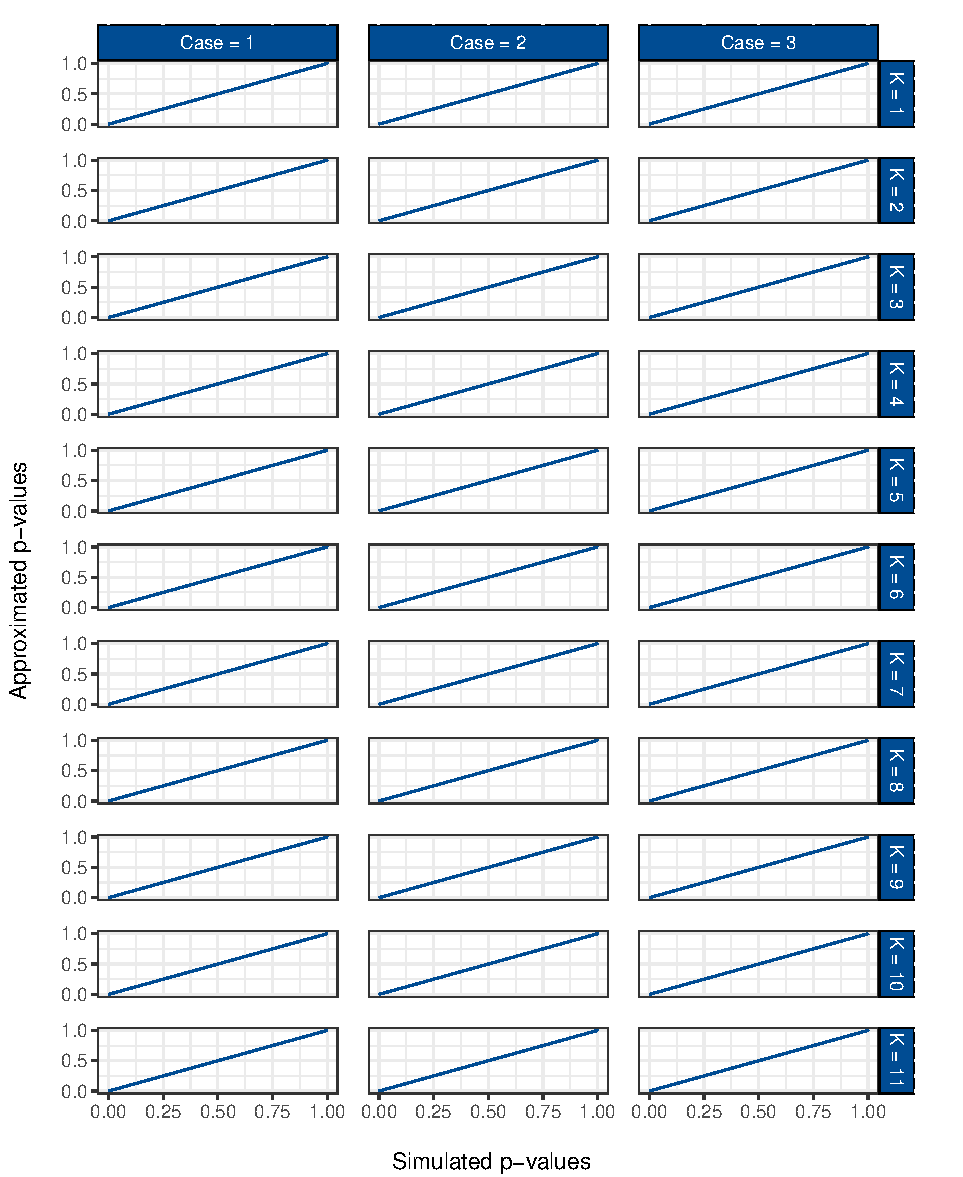
\includegraphics{p_approx_paper_files/figure-latex/approx_sim-all-1.pdf}
\caption{\label{fig:sim_approx_all} Simulated against approximated
\(p\)-values over the whole distribution for all cases and all
underlying tests.}
\end{figure}

\begin{figure}
\centering
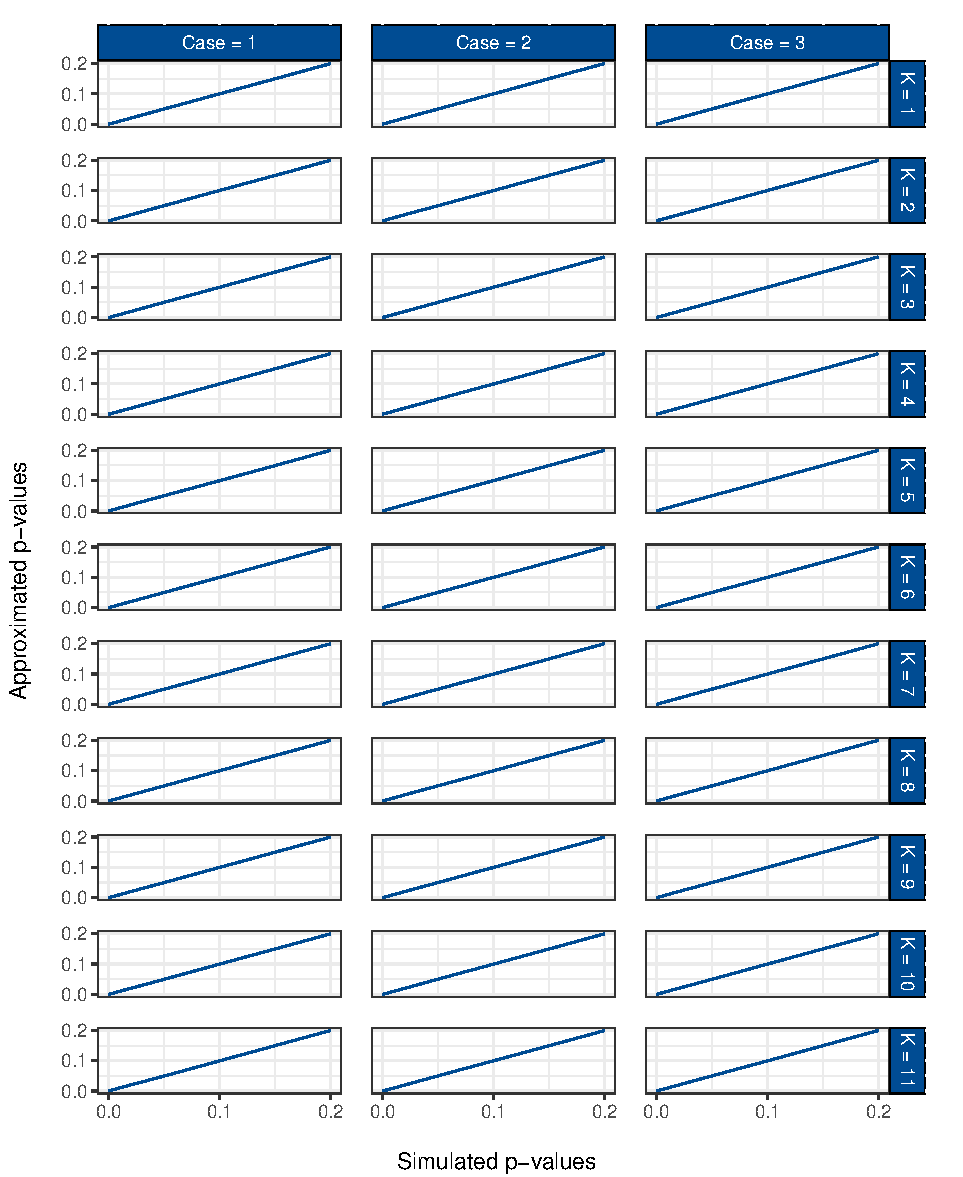
\includegraphics{p_approx_paper_files/figure-latex/approx_sim-all_0.2-1.pdf}
\caption{\label{fig:sim_approx_all_0.2} Simulated vs.~approximated
\(p\)-values for the lower tail of the distribution for all cases and
all underlying test.}
\end{figure}

\begin{figure}
\centering
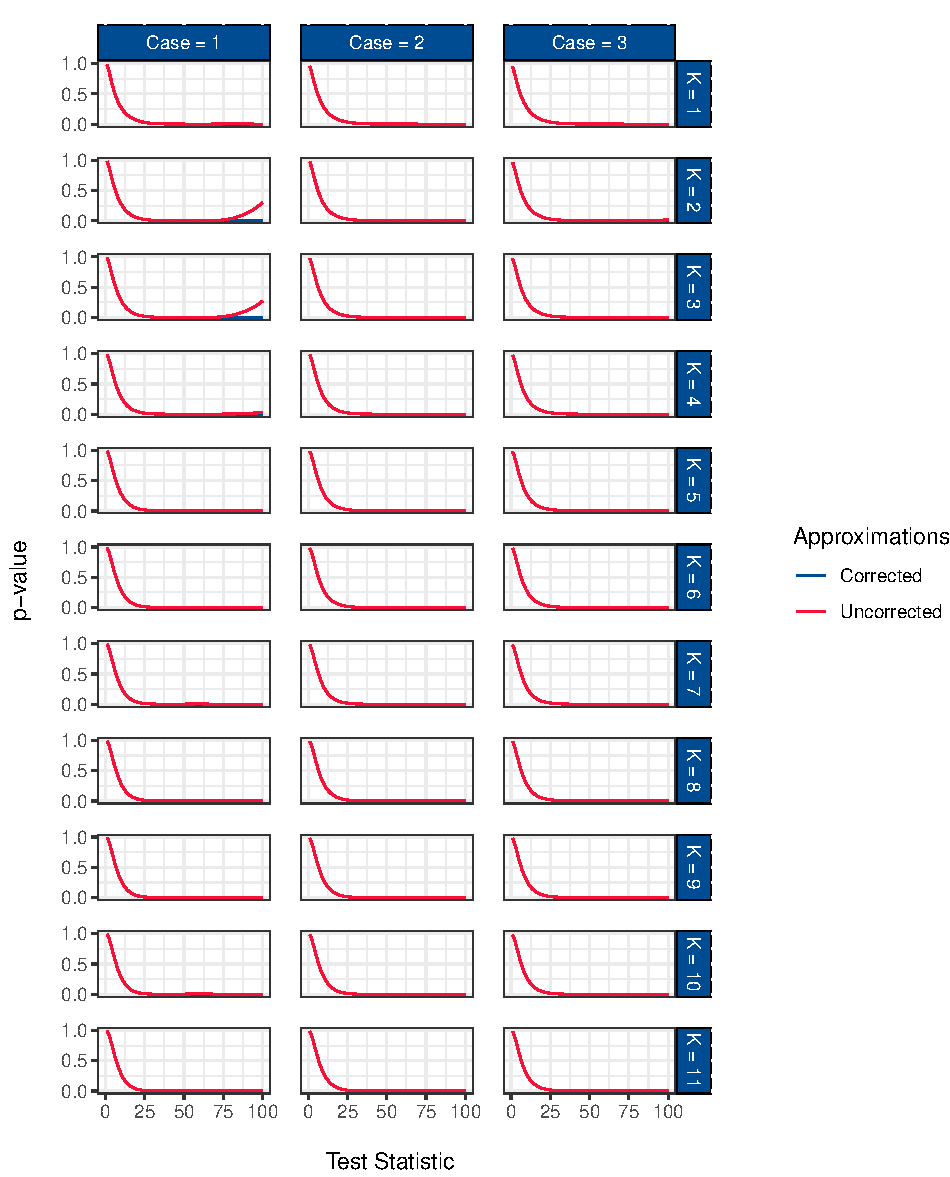
\includegraphics{p_approx_paper_files/figure-latex/p_stat_all-1.pdf}
\caption{\label{fig:fig_3} Corrected (blue) and uncorrected (red)
\(p\)-value predictions for all cases and all underlying tests.}
\end{figure}

\begin{figure}
\centering
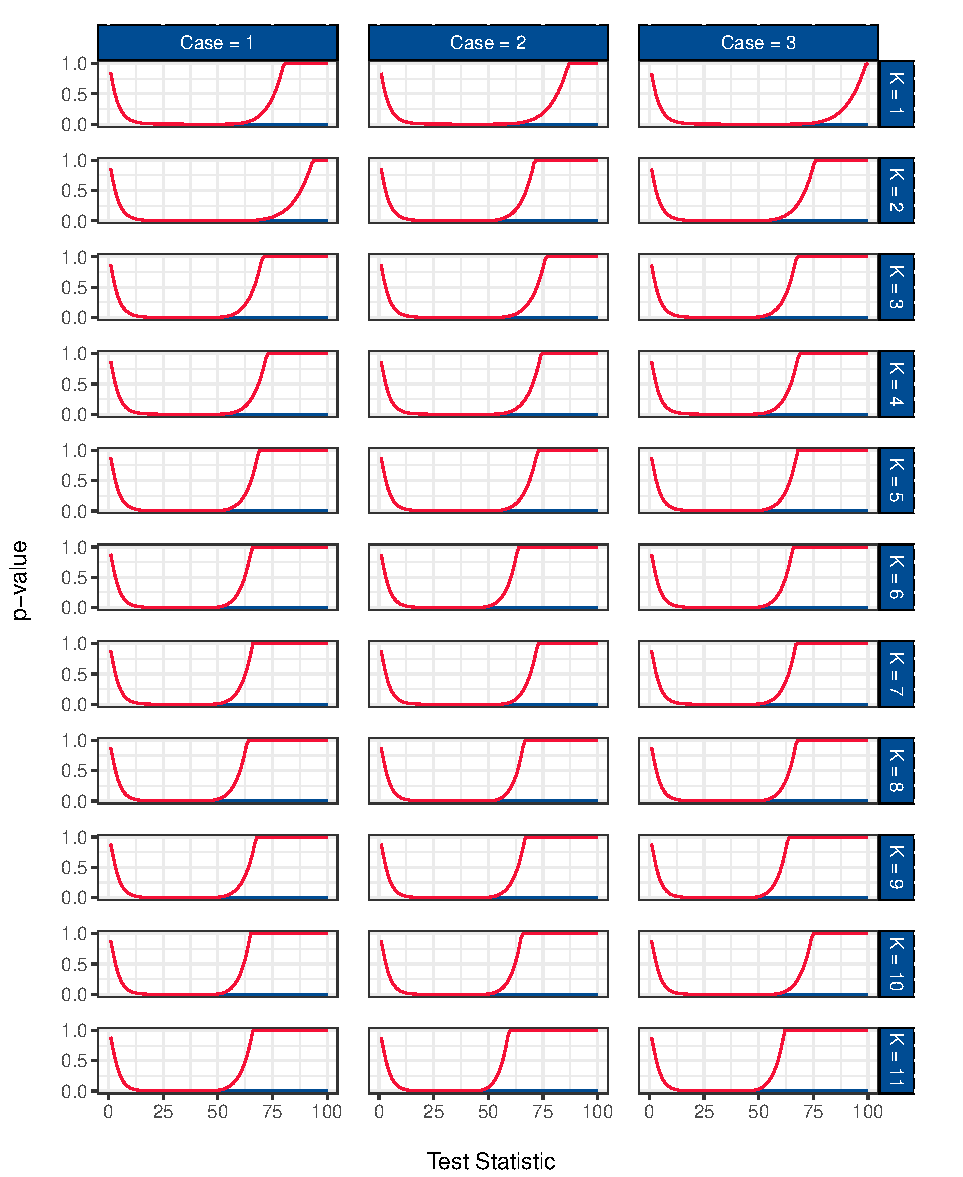
\includegraphics{p_approx_paper_files/figure-latex/p_stat_e_j-1.pdf}
\caption{\label{fig:fig_4} Corrected (blue) and uncorrected (red)
\(p\)-value predictions for all cases using Engle-Granger and Johansen
as underlying tests.}
\end{figure}

\restoregeometry

\cleardoublepage
\newpage
\renewcommand*{\mkbibnamefamily}[1]{\textbf{#1}}
\renewcommand*{\mkbibnamegiven}[1]{\textbf{#1}}
\renewcommand*{\mkbibnameprefix}[1]{\textbf{#1}}
\renewcommand*{\mkbibnamesuffix}[1]{\textbf{#1}}


% \printbibliography[title=References]
%\pagenumbering{arabic}


\newpage
\textbf{Eidesstattliche Versicherung}

\bigskip

Ich versichere an Eides statt durch meine Unterschrift, dass ich die vorstehende Arbeit selbständig und ohne fremde Hilfe angefertigt und alle Stellen, die ich wörtlich oder annähernd wörtlich aus Veröffentlichungen entnommen habe, als solche kenntlich gemacht habe, mich auch keiner anderen als der angegebenen Literatur oder sonstiger Hilfsmittel bedient habe. Die Arbeit hat in dieser oder ähnlicher Form noch keiner anderen Prüfungsbehörde vorgelegen.

\vspace{1cm}
\rule{0pt}{2\baselineskip} %
\par\noindent\makebox[2.25in]{\indent Essen, den \hrulefill} \hfill\makebox[2.25in]{\hrulefill}%
\par\noindent\makebox[2.25in][l]{} \hfill\makebox[2.25in][c]{Jens Klenke
and Janine Langerbein}%


\end{document}
